%%
\documentclass[english, 12pt, a4paper, elec, utf8, a-1b, online]{aaltothesis}

\usepackage{graphicx}
\usepackage{amsfonts,amssymb,amsbsy,amsmath}
\usepackage{biblatex}
\usepackage[vlined, ruled, linesnumbered, commentsnumbered]{algorithm2e}
\usepackage{multirow}

\usepackage{calc} % To reset the counter in the document after title page
\usepackage{bbm}
\usepackage{amsfonts,amssymb,amsbsy,amsmath}
\usepackage{mathtools}
\usepackage[inline]{enumitem}
\usepackage{bm}
\usepackage[vlined, ruled, linesnumbered, commentsnumbered]{algorithm2e}
\usepackage{caption}
\usepackage{subcaption}
\usepackage{gensymb}
\usepackage{outlines}
\usepackage{longtable}

\setlist[itemize]{itemsep=0.1ex, topsep=0.8ex}
\setlist[enumerate]{itemsep=0.1ex, topsep=0.8ex}


\addbibresource{references.bib}

\renewcommand{\vec}[1]{\mathbf{#1}}
\renewcommand{\Vec}[1]{\boldsymbol{#1}}

\newcommand{\tr}[1]{\texttt{Tr}\left\{ #1 \right\}}
\newcommand{\Pest}{P_{t+1|t}^{(k)}}
\newcommand{\etal}{\textit{et al}.~}
\newcommand{\Epolicy}[1]{\mathrm{E}_\pi \left[ #1 \right]}
\newcommand{\Ss}{\mathcal{S}}
\newcommand{\As}{\mathcal{A}}
\newcommand{\Rs}{\mathcal{R}}
\newcommand{\Ps}{\mathcal{P}}
\newcommand{\Os}{\Omega}
\newcommand{\Op}{O}
\newcommand{\argmax}{\text{argmax}}
\newcommand{\egreedy}{$\epsilon$-greedy~}
\newcommand{\E}[1]{\mathbb{E}\left[ #1 \right]}
\newcommand{\inv}[1]{#1^{-1}}
\newcommand{\sqinv}[1]{#1^{-\frac{1}{2}}}
\renewcommand{\Pr}[1]{\text{Pr}\left\{ #1 \right\}}

\newcommand{\xprior}{\hat{\vec{x}}_{k|k-1}}
\newcommand{\xpost}{\hat{\vec{x}}_{k|k}}
\newcommand{\xlast}{\hat{\vec{x}}_{k-1|k-1}}

\newcommand{\priorecov}{\boldsymbol{\Sigma}_{k|k-1}}
\newcommand{\postecov}{\boldsymbol{\Sigma}_{k|k}}
\newcommand{\lastecov}{\boldsymbol{\Sigma}_{k-1|k-1}}
\newcommand{\ecov}{\boldsymbol{\Sigma}_k}

\newcommand{\prefitinnov}{\vec{y}_k}
\newcommand{\postfitinnov}{\Tilde{\vec{y}}_{k|k}}

\newcommand{\x}{\vec{x}_k}
\newcommand{\xnext}{\vec{x}_{k+1}}
\newcommand{\xhat}{\hat{\vec{x}}_k}

\newcommand{\z}{\vec{z}_k}
\newcommand{\znext}{\vec{z}_{k+1}}

\newcommand{\stmodel}{\vec{F}_k}
\newcommand{\cimodel}{\vec{B}_k}
\newcommand{\cinput}{\vec{u}_k}
\newcommand{\pnoise}{\vec{w}_k}
\newcommand{\omodel}{\vec{H}_k}

\newcommand{\onoise}{\vec{v}_k}
\newcommand{\ocov}{\vec{R}_k}
\newcommand{\pcov}{\vec{Q}_k}
\newcommand{\innocov}{\vec{S}_k}

\newcommand{\eye}{\vec{I}}
\newcommand{\gain}{\vec{K}_k}

\newcommand{\normal}[2]{\mathcal{N}\left(#1, #2 \right)}
\newcommand{\xnormal}[3]{\mathcal{N}\left(#1; #2, #3\right)}

\newcommand{\Pd}{P_\text{D}}
\newcommand{\Pfa}{P_\text{FA}}
\newcommand{\SNR}{\text{SNR}}
\newcommand{\SN}{\text{SN}_0}

\renewcommand{\exp}[1]{\text{exp}\left( #1 \right)}
\newcommand{\transpose}[1]{#1^\text{T}}
\newcommand{\rotmat}{\mathbf{T}}

\newcommand{\tmax}{t_\text{max}}
\newcommand{\tmin}{t_\text{min}}
\newcommand{\nmax}{n_\text{max}}
\newcommand{\muca}{\mu_{\text{CA}}}
\newcommand{\mucv}{\mu_{\text{CV}}}

\newcommand{\stprobs}{\vec{P}}

\newcommand{\modeprob}{\mu_k^i}
\newcommand{\lastmxprobs}{\mu^{j|i}_{k-1|k-1}}
\newcommand{\mxnorm}{ \Bar{c}_i }
\newcommand{\xmxinit}{\hat{\vec{x}}^{0i}_{k-1|k-1}}
\newcommand{\xmxinitcurr}{\hat{\vec{x}}^{0i}_{k|k}}
\newcommand{\ecovmxinit}{\bm{\Sigma}^{0i}_{k-1|k-1}}
\newcommand{\ecovmxinitcurr}{\bm{\Sigma}^{0i}_{k|k}}
\newcommand{\modexlast}{\hat{\vec{x}}^{j}_{k-1|k-1}}
\newcommand{\modexprior}{\hat{\vec{x}}^{i}_{k|k-1}}
\newcommand{\modecovlast}{\bm{\Sigma}^j_{k-1|k-1}}
\newcommand{\modecovprior}{\bm{\Sigma}^i_{k|k-1}}
\newcommand{\modeinnovcov}{\mathbf{S}^i_{k}}
\newcommand{\modemxcovlast}{\Tilde{\bm{\Sigma}}^{ij}_{k-1|k-1}}
\newcommand{\modexpost}{\hat{\vec{x}}^{i}_{k|k}}
\newcommand{\modecovpost}{\bm{\Sigma}^i_{k|k}}
\newcommand{\modeobsprob}{\Lambda^i_k}

\newcommand{\priorecovth}{\bm{\Sigma}_{\text{th}}}

\newcommand{\deltalim}{\Delta_\text{lim}}
\newcommand{\Asdir}{\As_\text{D}}
\newcommand{\Asdelta}{\As_\Delta}

\def\prior{\textit{a priori}\ }
\def\post{\textit{a posteriori}\ }
\newcommand{\zhat}{\hat{\vec{z}}_k}

\newcommand{\mimm}{\mathcal{M}}

\newcommand{\nacts}{{N_\text{a}}}
\newcommand{\nstates}{{N_\text{s}}}
\newcommand{\nmodels}{{N_\text{m}}}

\newcommand{\real}{\mathbb{R}}

\newcommand{\dt}{\Delta t}

\newcommand{\uqos}{u_\text{QoS}}
\newcommand{\closs}{c_\text{loss}}


% --- MAB paper commands --- 
\newcommand{\bo}[1]{\boldsymbol{\mathrm{#1}}}
\newcommand{\norm}[1]{\lVert#1\rVert}
\newcommand{\Norm}[1]{\big \lVert#1\big\rVert}
\newcommand{\NORM}[1]{\left \lVert#1\right\rVert}
\newcommand{\abs}[1]{\lvert#1\rvert}
\newcommand{\Abs}[1]{\Big \lvert#1\Big \rvert}
\newcommand{\ABS}[1]{\bigg \lvert#1\bigg \rvert}
\newcommand{\re}{\mathrm{Re}}
\newcommand{\im}{\mathrm{Im}}
\newcommand{\diag}[1]{\text{diag}\left\{ #1 \right\}}
\newcommand{\dd}{\mathrm{d}}
\newcommand{\set}[1]{\mathcal{#1}}
\newcommand{\iu}{\mathfrak{j}}
\newcommand{\Var}[1]{\text{Var}\left[ #1 \right]}


\newcommand{\thnoise}{\sigma^2_{\text{th}}}

\newcommand{\epower}{p_{m}}
\newcommand{\vpower}{\boldsymbol{p}}

\newcommand{\eintnoise}{\sigma^2_{\text{int}_{n}}}
\newcommand{\vintnoise}{\boldsymbol{\sigma}^2_{\text{int}}}

\newcommand{\esinr}{\gamma_{{nm}}}
\newcommand{\vsinr}{\boldsymbol{\gamma}}

\newcommand{\esinrexp}{\Gamma_{nm}}
\newcommand{\vsinrexp}{\boldsymbol{\Gamma}}

\newcommand{\esinrb}{\widehat{\Gamma}_{nm}}
\newcommand{\vsinrb}{\widehat{\boldsymbol{\Gamma}}}

\newcommand{\ereward}{r^t_a}
\newcommand{\vreward}{\boldsymbol{r}^t}

\newcommand{\brewardb}{B^{t_k}}
\newcommand{\vrewardb}{\boldsymbol{B}^t}

\newcommand{\epl}{L_{nm}}
\newcommand{\vpl}{\boldsymbol{L}}

\newcommand{\ercs}{\psi_{nm}}
\newcommand{\vrcs}{\boldsymbol{\psi}}

\newcommand{\fl}{c(t)}

\newcommand{\easvtx}{\delta_{\text{tx}_m}}
\newcommand{\vasvtx}{\boldsymbol{\delta}_{\text{tx}}}
\newcommand{\easvrx}{\delta_{\text{rx}_n}}
\newcommand{\vasvrx}{\boldsymbol{\delta}_{\text{rx}}}
\newcommand{\vsp}{\boldsymbol{\rho}}
\newcommand{\esp}{\rho_{nm}}

\newcommand{\eindex}{X_{nm}}
\newcommand{\vindex}{\boldsymbol{X}}

\newcommand{\ri}{t_r}

\DeclarePairedDelimiter\ceil{\lceil}{\rceil}
\DeclarePairedDelimiter\floor{\lfloor}{\rfloor}


\degreeprogram{Computer, Communication and Information Sciences}
\major{Signal, Speech and Language Processing}
\code{ELEC3031}
\univdegree{MSc}
\thesisauthor{Petteri Pulkkinen}
\thesistitle{Reinforcement Learning Methods for Radar Resource Management}
\place{Espoo}
\date{1.6.2020}
\supervisor{Prof.\ Visa Koivunen}
\advisor{Dr Tuomas Aittomäki}


%% \uselogo{aaltoRed|aaltoBlue|aaltoYellow|aaltoGray|aaltoGrayScale}{?|!|''}
\uselogo{aaltoBlue}{''}

\keywords{reinforcement learning\spc radar}

\thesisabstract{
Your abstract in English. Keep the abstract short. The abstract explains your 
research topic, the methods you have used, and the results you obtained. In the 
PDF/A format of this thesis, in addition to the abstract page, the abstract text is 
written into the pdf file's metadata. Write here the text that goes into the 
metadata. The metadata cannot contain special characters, linebreak or paragraph 
break characters, so these must not be used here. If your abstract does not contain 
special characters and it does not require paragraphs, you may take advantage of 
the abstracttext macro (see the comment below). Otherwise, the metadata abstract 
text must be identical to the text on the abstract page.
}

\copyrighttext{Copyright \noexpand\copyright\ \number\year\ \ThesisAuthor}
{Copyright \copyright{} \number\year{} \ThesisAuthor}


%% All that is printed on paper starts here
%%
\begin{document}

%% Create the coverpage
%%
\makecoverpage

%% Typeset the copyright text.
%% If you wish, you may leave out the copyright text from the human-readable
%% page of the pdf file. This may seem like a attractive idea for the printed
%% document especially if "Copyright (c) yyyy Eddie Engineer" is the only text
%% on the page. However, the recommendation is to print this copyright text.
%%
\makecopyrightpage

%% Note that when writting your thesis in English, place the English abstract
%% first followed by the possible Finnish or Swedish abstract.

%% Abstract text
%% All the details (name, title, etc.) on the abstract page appear as specified
%% above.
%%
\begin{abstractpage}[english]
  Your abstract in English. Keep the abstract short. The abstract explains your
  research topic, the methods you have used, and the results you obtained.  
  
  The abstract text of this thesis is written on the readable abstract page as
  well as into the pdf file's metadata via the $\backslash$thesisabstract macro
  (see above). Write here the text that goes onto the readable abstract page.
  You can have special characters, linebreaks, and paragraphs here. Otherwise,
  this abstract text must be identical to the metadata abstract text.
  
  If your abstract does not contain special characters and it does not require
  paragraphs, you may take advantage of the abstracttext macro (see the comment
  below).
\end{abstractpage}

\newpage
%%
%% Abstract in Finnish.  Delete if you don't need it. 
%%
\thesistitle{Vahvistusoppimismetodit tutkan resurssienhallinnassa}
\supervisor{Prof.\ Visa Koivunen}
\advisor{TkT Tuomas Aittomäki}
\degreeprogram{Tietojenkäsittely, Tietotekniikka ja Informaatioteknologia}
%\department{Elektroniikan ja nanotekniikan laitos}
\major{Signaalin-, Puheen- ja Kielenkäsittely}
\keywords{Vahvistusoppiminen \spc tutka}
%% Abstract text
\begin{abstractpage}[finnish]
  Tiivistelmässä on lyhyt selvitys
  kirjoituksen tärkeimmästä sisällöstä: mitä ja miten on tutkittu,
  sekä mitä tuloksia on saatu. 
\end{abstractpage}

%% Force new page so that the Swedish abstract starts from a new page
\newpage

%% Preface
%%
%% This section is optional. Remove it if you do not want a preface.
\mysection{Preface}

\vspace{5cm}
Otaniemi, 1.6.2020

\vspace{5mm}
{\hfill Petteri T.\ Pulkkinen \hspace{1cm}}

\newpage

%% Table of contents. 
%%
\thesistableofcontents


%% Symbols and abbreviations
\mysection{Symbols and abbreviations}

\subsection*{Symbols}

\begin{longtable}{ll}
% -----------------------
% General symbols
% -----------------------
$k$ & time index \\
$t_k$ & time at time instance $k$ \\
&\\
% -----------------------
% RL/MDP/POMDP related symbols
% -----------------------
$\nstates$ & number of all possible states \\
$\Ss$ & set of all possible states, i.e state space \\
$s_i$ & state, indexed by $i \in \{1, ..., \nstates\}$ \\
$S_k$ & state at time instance $k$ \\
&\\
$\nacts$ & number of all possible actions \\
$\As$ & set of all possible actions, i.e action space \\
$\As_s$ & set of possible actions given the state $s \in \Ss$ \\
$a_i$ & action, indexed by $i \in \{1, ..., \nacts\}$ \\
$A_k$ & action at time instance $k$ \\
&\\
$\Rs$ & set of all possible rewards \\
$\Rs_{ss'}^a$ & set of possible rewards for action $a$ given state transition from $s$ to $s'$ \\
$R_k$ & reward at time instance $k$ \\
&\\
$\stprobs$ & state transition probability matrix \\
$p_{ij}$ & element of $\stprobs$ in row $i$ and column $j$ \\
$\stprobs_a$ & state transition probability matrix given action $a \in \As$ \\
$p_{ij}^a$ & element of $\stprobs_a$ in row $i$ and column $j$ \\
&\\
$\Os$ & set of all possible observations, i.e. observation space \\
$\Os_s^a$ & set of possible observations given action $a \in \As_s$ and state $s \in \Ss $ \\
$z$ & observation \\
$Z_k$ & observation sequence until time instance $k$ \\
$\Op(z | s, a)$ & probability of observing $z \in \Os_s^a$ given state $s_i \in \Ss$ and action $a \in \As_s$ \\
$b_k$ & belief state at time instance $k$ \\
$b_k(s)$ & probability of being on state $s \in \Ss$ at time instance $k$ \\

&\\
$\pi$ & policy \\
$\pi^*$ & optimal policy \\
$\pi(a|s)$ & probability of taking action $a \in \As_s$ given state $\Ss$ \\
$v_\pi(s)$ & value for state $s$ under policy $\pi$ \\
$q_\pi(s, a)$ & value for action $a \in \As_s$ and state $s \in \Ss$ under policy $\pi$ \\
$G_k$ & discounted sum of rewards \\
$\lambda$ & discount factor \\
$\epsilon$ & probability of random action in \egreedy policy \\
&\\
% -----------------------
% KF related symbols
% -----------------------
$\stmodel$ & state-transition matrix at time instance $k$\\
$\pnoise$ & process noise at time instance $k$\\
$\omodel$ & observation matrix at time instance $k$\\
$\onoise$ & observation noise at time instance $k$\\
$\cinput$ & control input at time instance $k$\\
$\cimodel$ & control input matrix at time instance $k$\\
$\pcov$ & process noise covariance matrix at time instance $k$\\
$\ocov$ & observation noise covariance matrix at time instance $k$\\
&\\
$\x$ & kinematic state of a target at time instance $k$ \\
$\z$ & radar observation at time instance $k$ \\
$\zhat$ & predicted radar observation at time instance $k$ \\
$\prefitinnov$ & innovation at time instance $k$ \\
$\xprior$ & \prior (predicted) estimate of state $\x$\\
$\xpost$ & \post (filtered) estimate of state $\x$ \\
$\priorecov$ & prediction error covariance matrix on estimate $\xprior$ \\
$\postecov$ & filtering error covariance matrix on estimate $\xpost$ \\
$\gain$ & Kalman gain at time instance $k$ \\
$\innocov$ & Innovation covariance matrix at time instance $k$ \\
&\\
% -----------------------
% IMM related symbols
% -----------------------
$\nmodels$ & number of maneuvering models \\
$\mimm$ & set of maneuvering models \\
$m_i$ & maneuvering model, indexed by $i \in \{1, ..., \nmodels\}$ \\
$M_k$ & maneuvering model at time instance $k$ \\
$\modeprob$ & maneuver model probability for model $m_i \in \mimm$ at time instance $k$ \\
$\xmxinitcurr$ & mixed \post (filtered) estimate of $\x$ for model $m_i \in \mimm$\\
$\ecovmxinitcurr$ & estimated error covariance matrix on estimate $\xmxinitcurr$\\
&\\
% -----------------------
% revisit interval selection related symbols
% -----------------------
$\ri$ & revisit interval \\
$\tau_d$ & dwell length \\
&\\
% -----------------------
% RL for revisit interval related symbols
% -----------------------
$\Asdir$ & set of possible actions for direct revisit interval selections \\
$\Asdelta$ & set of possible actions for delta revisit interval selections \\
$\deltalim$ & maximum increase or decrease in delta revisit interval action \\
\end{longtable}

\subsection*{Abbreviations}

\begin{tabular}{ll}
AESA & Adaptive Electronically Scanned Arrays \\
FTS & Fast time scale \\
HMM & Hidden Markov Model \\
IMM & Interacting Multiple Model \\
JMLS & Jump Markov linear system \\
LSTM & Long short-term memory \\
MDP & Markov decision process \\
MSE & Mean square error \\
POMDP      & Partially observable Markov decision process \\
PLT & Probability to lose a track \\
RL & Reinforcement learning \\
RI  & Revisit interval \\
RIS & Revisit interval selection \\
STS & Slow time scale \\
TBM & Time budget management \\
\end{tabular}


\cleardoublepage

\section{Introduction}


Reinforcement learning (RL) refers to subfield of machine learning methods that enable software agents to learn from interaction while not using any model developed beforehand \cite{Sutton2018}. 
Over the last decade, RL has generated a great interest in the research community due to various improvements in RL algorithms. 
Specifically, deep learning techniques have enabled applying RL to application domains that were considered too difficult before. 
Deep reinforcement learning algorithms have been applied to solve many tasks in communications and networking applications \cite{Luong2018} as well as in robotics \cite{Kober2013} and smart grids \cite{Zhang2018}. 


Radar (RAdio Detection And Ranging) is a sensing system which is used to detect targets using radio waves \cite{Curry2011}.
Despite the obvious advantages of the RL methods, those have not yet been researched as extensively for radar applications.
Radar resource management (RRM) considers managing radar resources such as time, energy, and processing budget as well as selecting operational parameters of the radar \cite{Moo2016}. 
A general RRM problem can be divided into numerous subproblems which are typically solved by using models for the radar, the environment, and the target.
However, the models are typically non-optimal for real-world radar scenarios, thus algorithms using the models are vulnerable for modeling errors and inconsistencies.  
This issue can be addressed by applying RL to replace or improve existing RRM algorithms. 
RL would allow radar systems to learn in real-time from experience such that the modelling errors could be avoided. 

Current research for applying RL to RRM considers
jamming strategies \cite{Qiang2017, Wang2019, Wang2019a, Zhang2019},
anti-jamming strategies \cite{Kang2018, Ak2019}, 
bandwidth allocation in environments with interfering communications system \cite{Selvi2018, Kozy2019},
selecting transmit frequency to improve detection performance in environments with clutter \cite{Wabeke2010}, 
information-theoretic beam scheduling for multitarget tracking \cite{Kreucher2005, Xu2010},
a low-level scheduling algorithm for multichannel multifunction radars \cite{Shaghaghi2018},
selecting the number of angle cells to be included into a beam pattern in colocated Multiple-Input Multiple-Output (MIMO) radar \cite{Wang2018}, 
and a sequential operation mode selection to improve detection performance for moving radar platform \cite{Smits2008}.
Thus, most of the RL related research considers selecting  either frequency or bandwidth. 
However, many RRM subproblems have not been addressed, including transmitter (TX) and receiver (RX) selection in distributed MIMO radars \cite{Godrich2011a, Godrich2011, Sun2014}, and revisit interval selection (RIS) which is related to radar time budget management (TBM) \cite{Cohen1986, Gardner1988, Munu1992, ChengTing2007, Baek2010, Watson1993, Charlish2015, Keuk1975, Shin1995, Benoudnine2006, Esfahani2012}.

The aim of this thesis is to formulate RRM subproblems as RL problems in order to identify if learning based approaches can improve the performance of radar systems by enabling them to learn from past experience. 
To evaluate the RL based RRM solutions, the proposed RL approaches and model-based approaches are compared using Monte Carlo simulations. 
This thesis focuses on two explicit RRM subproblems that have not been addressed by RL methods before. 
The two considered subproblems are the TX-RX selection problem for distributed MIMO radars, and the RIS problem.
TX-RX selection is addressed by utilizing multi-armed bandit framework which is developed for problems solely concentrating on the exploration-exploitation trade-off. 
RIS is formulated as a general RL problem which is solved by using Q-learning algorithm.
It will be shown that the considered RRM subproblems can be addressed using RL methods and furthermore that the performance can be improved by enabling the radar system to learn in real-time.
However, only single target tracking (STT) scenarios are considered which simplifies the RL formulations. 

The thesis is structured as follows. Chapter \ref{sec:background} describes principles of radars and target tracking. Chapter \ref{sec:RL} reviews the theory on RL that is important to understand the proposed RL approach. 
Chapter \ref{sec:existing_RRM} explains the considered RRM subproblems in detail and describes existing solutions.
The RL approach for distributed MIMO radar TX-RX selection is formulated and evaluated in Chapter \ref{sec:RL_TX_RX}. Moreover,  Chapter \ref{sec:rl_ri} introduces the RL formulation for the RIS problem and the approach is evaluated against baseline algorithm. 
Finally, Chapter \ref{sec:conclusions} draws conclusions about the suitability of using RL for the considered RRM subproblems. 


\clearpage
\section{Radar systems}\label{sec:background}

Radar resource management (RRM) stands for controlling any of the degrees of freedom (DoF) parameters of the radar or allocating radar resources, such as power, bandwidth and time, for a specific radar task.
This chapter provides an overview of radar systems and underlying theory and methods to give background for the considered RRM problems.
Section \ref{sec:radar_opertaion_principle} briefly introduces the operation principle of a radar.
Different radar types are briefly described in Section \ref{sec:radar_types}. 
The RRM problems to be solved typically depend on the specific radar type. 
Finally, Section \ref{sec:Tracking} covers basic concepts of target tracking because the target tracking is one of the key radar tasks which involves many RRM problems.

\subsection{Operation principles of radars} \label{sec:radar_opertaion_principle}

\begin{figure}[htb]
    \centering
    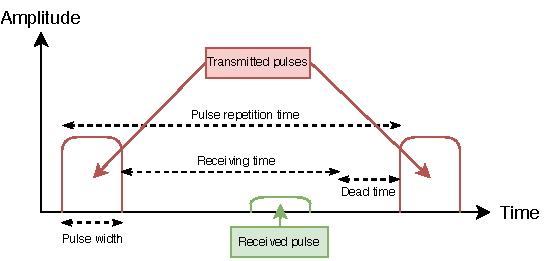
\includegraphics[width=0.8\textwidth]{figures/background/pulsed_radar.pdf}
    \caption{Pulsed radar time amplitude figure.}
    \label{fig:pulsed_radar}
\end{figure}

Radar (RAdio Detection And Ranging) is a sensing system which is used to detect targets using radio waves \cite{Curry2011}.
Transmitter (TX) emits radio waves towards desired directions, and a receiver (RX) is used to receive radio waves reflected from surfaces and scattered off the targets. 
The reflected or scattered waves are often called echoes.
Radar cross section (RCS) determines the fraction of electromagnetic energy that is scattered from the target in direction of the receiver \cite{Curry2011}.
The target RCS depends on target shape and materials as well as on radar frequency, viewing angles, and signal polarization.
The target RCS has unit of square meter sm (or m$^2$) and often described in decibels by dBsm.

The echoes produced by from other sources than targets of interest are called clutter.
The received signal is corrupted by clutter, additive noise from the receiver electronics, and possible also unintentional or intentional interferences from other radio systems.
In modern radar systems, signal processing algorithms are utilized to perform target detection from the corrupted received signal \cite{Mahafza2015}.
Typical detection algorithm is based on matched filtering and hypothesis testing \cite{Mahafza2015}.

There are two types of radar systems when categorized based on the waveform used.
These systems are pulsed wave radar systems and continuous wave (CW) radar systems.  \cite{Mahafza2015}.
Only pulsed wave radar systems are considered in rest of the thesis.
The target range is obtained by measuring the time taken by a radio wave to propagate from a TX via target to an RX.
For a radar which has TX and RX at the same location, the range is obtained using the following equation \cite{Curry2011}
\begin{equation}
    d = \frac{ c\dt}{2} 
\end{equation}
where $\dt$ is the time delay and $c$ is speed of light.
A range-rate, i.e. the radial velocity component towards or away from the receiver, is obtained by utilizing the Doppler shift induced to the received radio wave.
When the frequency shift of the received signal is $f_d$, the range-rate is obtained using the following equation \cite{Curry2011}
\begin{equation}
    v_r = \frac{cf_d}{2f_c}
\end{equation}
where $f_c$ is frequency of the transmitted waveform.


Pulsed wave radar systems sense the space by transmitting a train of pulses \cite{Mahafza2015}.
Figure \ref{fig:pulsed_radar} illustrates the transmitted pulses and received echoes.
The time between subsequent pulses is called pulse repetition time (PRT). 
Furthermore, pulse repetition frequency (PRF) stands for reciprocal of PRT.
As shown in Figure \ref{fig:pulsed_radar}, PRT is determined by pulse duration, receiving time and dead time.
pulse duration affects to the amount of energy that will be transmitted.
With higher energy, it is easier to detect the targets.
The pulse duration also affects the range resolution which defines how well two closely spaced targets can be separated.
Receiving time determines the maximum unambiguous range detectable by the radar.
If the target is at longer range than the maximum unambiguous range, the received pulse is not the most recent transmitted pulse such that the propagation delay $\dt$ could not be correctly calculated.
Lastly, radars require a dead time for transitioning from a receiving mode to a transmission mode.
The dead time is used for internal checks and steering the electromagnetic energy into correct direction.

Signal-to-noise ratio (SNR) of the radar can be calculated using the following equation \cite{Curry2011}
\begin{equation} \label{eq:radar_snr}
SNR = \frac{P_p \tau G_T \sigma G_R \lambda^2 C}{(4\pi)^3 R_T^2 R_R^2 k T_s L},
\end{equation}
where
\begin{itemize}
    \item $P_p$ is the peak transmit power,
    \item $G_T$ is the transmit antenna gain,
    \item $\sigma$ is the target RCS,
    \item $G_R$ is the receive antenna gain,
    \item $\lambda$ is the wavelength,
    \item $C$ is the pulse compression gain,
    \item $R_T$ is the target range from transmitter,
    \item $R_R$ is the target range from receiver,
    \item $k$ is Boltzmann's coefficient,
    \item $T_s$ is the system noise temperature, and 
    \item $L$ is the additional radar system loss factor.
\end{itemize}
Pulse compression gain $C >= 1$ depends on the waveform used.
The system loss factor $L$ includes any additional losses originated from the environment or the radar system.

Other factors that affect the SNR are interference and pulse integration.
Signals received by the radar but originating from outside the radar system are considered interference.
Thus, signal-to-interference-plus-noise ratio (SINR) has form of $\frac{S}{N+I}$, where
$I$ is the received power of the interference.
However, interference may also be intentional and have properties  different from random noise. 
Pulse integration denotes to combining multiple signal returns in order to get higher SNR.
The SNR gain factor depends on whether coherent or non-coherent integration is used.
Coherent integration means that phase information can be preserved, thus the returns can be integrated with aligned phases \cite{Curry2011}.

The radars steer the transmitted radio waves into desired direction either mechanically by rotating the transmit antenna, or using Electronically Steerable Arrays (ESA) which are based on a phased array technology.
Mechanically steerable radar systems typically rotate with constant angular velocity, such that each azimuth-elevation bin is revisited with constant revisit time.
An electronically steerable phased array can be steered to any direction with relative low delay within field of view (FOV).
Thus, RRM for ESA radars have more degrees of freedom for controlling the beampattern.


\subsection{Radar configurations} \label{sec:radar_types}

\begin{figure}[htb]
    \centering
    \begin{subfigure}[b]{0.45\textwidth}
        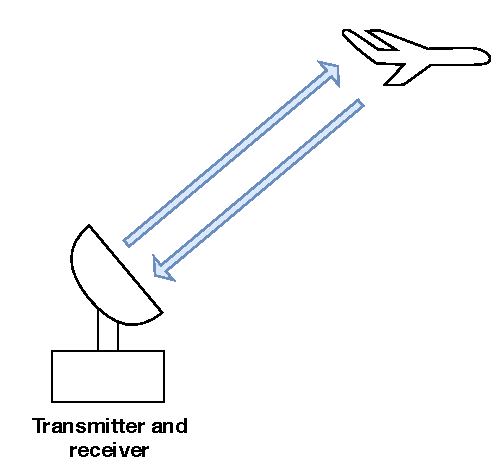
\includegraphics[width=0.7\textwidth]{figures/background/radar_types_monostatic.pdf}
        \caption{Monostatic radar.}
        \label{fig:monostatic_radar}
    \end{subfigure}
    \hfill
    \begin{subfigure}[b]{0.45\textwidth}
        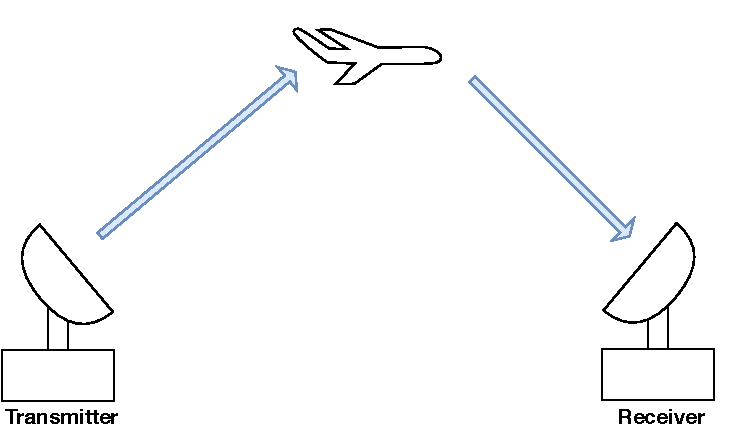
\includegraphics[width=\textwidth]{figures/background/radar_types_bistatic.pdf}
        \caption{Bistatic radar.}
        \label{fig:bistatic_radar}
    \end{subfigure}
    \hfill
    \begin{subfigure}[b]{0.45\textwidth}
        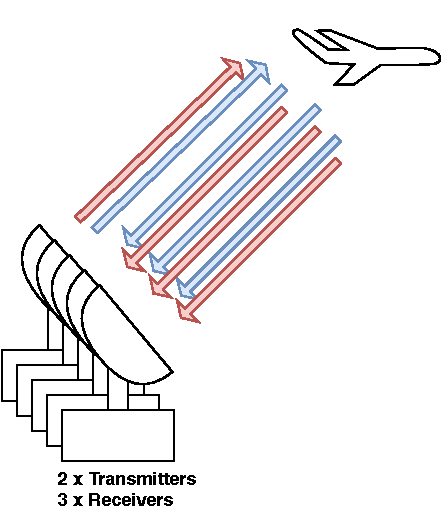
\includegraphics[width=0.7\textwidth]{figures/background/radar_types_colocated_MIMO.pdf}
        \caption{Example of MIMO radar with co-located antennas.}
        \label{fig:colocated_MIMO_radar}
    \end{subfigure}
    \hfill
    \begin{subfigure}[b]{0.45\textwidth}
        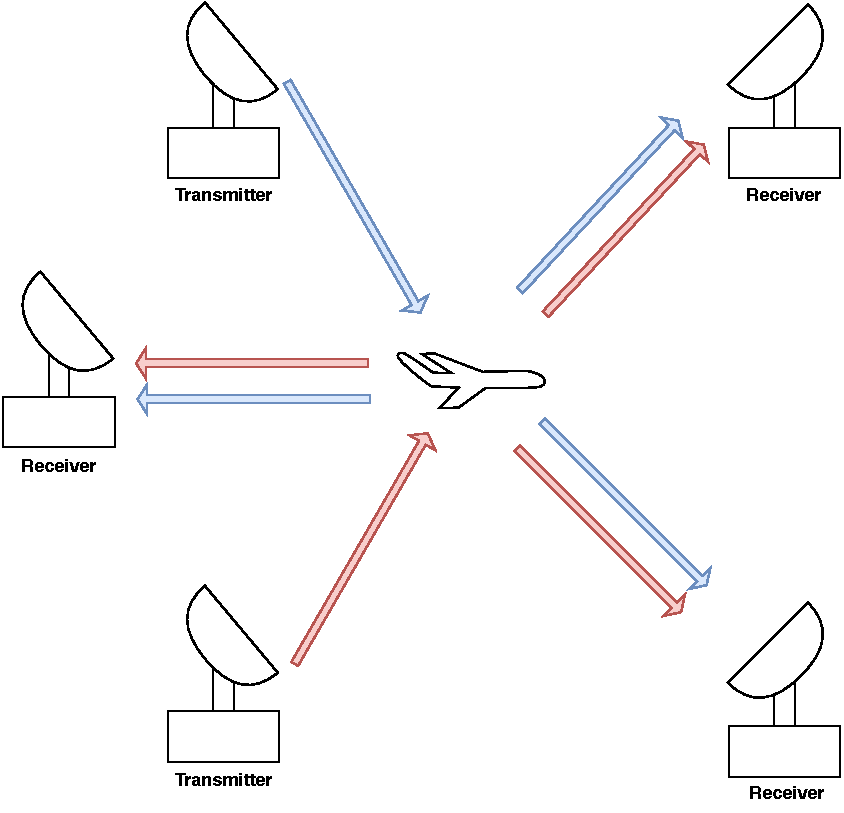
\includegraphics[width=\textwidth]{figures/background/radar_types_distributed_MIMO.pdf}
        \caption{Example of MIMO radar system with distributed antennas.}
        \label{fig:distributed_MIMO_radar}
    \end{subfigure}
    \caption{Different radar configurations. The arrows illustrate propagation of a waveform from a transmitter to a receiver.}
    \label{fig:radar_types}
\end{figure}

In general, radar systems can be divided into three configuration classes: monostatic radars, bistatic radars, and multistatic radars.
Monostatic radar systems have a single radio unit that can transmit and receive radio waves, as shown in Figure \ref{fig:monostatic_radar}.
Bistatic radar system has a TX unit and a RX unit which are distant from each other, as shown in Figure \ref{fig:bistatic_radar}.
Furthermore, multistatic radar system is a radar network that has multiple transmitters and receivers.
The individual radar components can be either monostatic radars or bistatic radars.
In conventional multistatic radar systems each radar component can function independently and only high level products of local processing is given for the central processor.

A specific subcategory of multistatic radar systems is multiple-input multiple-output (MIMO) radars \cite{Haimovich2008}.
The designation is used to distinguish the difference in designing and processing the multiple waveforms jointly, compared to the conventional multistatic radar systems.
Therefore, each transmitter-receiver (TX-RX) pair forms an independent
channel for illuminating and observing the targets.
MIMO radars can be further divided into the following subclasses: MIMO radars with colocated antennas, and MIMO radars with widely separated antennas.
The subclasses will be referred as co-located MIMO radars and distributed MIMO radars, respectively.

Colocated MIMO radars have multiple antennas closely located to each other.
Compared to phased-array monostatic radars, the MIMO radar technology improves the parameter estimation capabilities, and enhance the flexibility in transmit beampattern design \cite{Li2007}.
It may transmit multiple different waveforms simultaneously whereas phased-array radar sends the same waveform from each antenna with appropriate delay.
An example of a co-located MIMO radar with two TXs antennas and three RXs antennas is shown in Figure \ref{fig:colocated_MIMO_radar}.
In distributed MIMO radar systems, multiple TXs and RXs are deployed in different locations.
The distances between the antennas are larger than coherence distance such that the radar channels are not correlated \cite{Haimovich2008}.
The widely distributed antennas increase spatial diversity which can be utilized for improved target localization accuracy and detecting low-observable targets.
An example of a distributed MIMO radar with two TXs and three RXs is shown in Figure \ref{fig:distributed_MIMO_radar}.

\subsection{Target tracking with radars} \label{sec:Tracking}

Radars acquire observations that are processed to obtain for example the target position and the range-rate as discussed in Section \ref{sec:radar_opertaion_principle}.
A state of a target can be modeled as a continuous-valued stochastic process that evolves based on the target dynamics such as velocity, acceleration and maneuvering. 
Typically, the state variables are not directly observable since measurements may contain noise or all the state variables can not be observed.
Therefore, target tracking algorithms are utilized to filter the observation history to attenuate noise, as well as to estimate the present state and predict future states.
Typical target tracking algorithms are based on statistical model that combine a motion model and a measurement model. 
Such a models are known as state-space models \cite{RongLi2003}.

The motion model describes how the kinematic state of a target $\x$ evolves through time.
In general, the notation $\x$ is short hand for $\vec{x}_{t_k}$ which means value of $\vec{x}$ at time instant $t_k$. 
A discrete-time motion model may be expressed as
\begin{equation}\label{eq:spm_motion}
    \xnext  = f(\x, \cinput) + \pnoise,
\end{equation}
where $f(\x, \cinput)$ is a deterministic function the previous state $\x$ and the control input $\cinput$. 
The variable $\pnoise$ models noise that describes uncertainty in the model.
The measurement model is used to describe the relationship between the target state and the observation $\z$. 
Similar to the motion model, the discrete-time measurement model is written as follows,
\begin{equation}\label{eq:spm_obs}
    \z = h(\x) + \onoise,
\end{equation}
where $h(\z)$ maps the state to the observation, and $\onoise$ is the measurement noise.

\subsubsection{Target motion models} \label{sec:target_models}

Different kinds of target motion models have been developed to mimic the true target motion with desired accuracy. 
Commonly used motion models include constant velocity (CV), constant acceleration (CA) and oordinated turn (CT) models \cite{RongLi2003}.
On a higher level, the models can be divided into non-maneuvering and maneuvering models. 
Non-maneuvering motion means that the target velocity and elevation remain approximately constant, and otherwise the motion is considered as a maneuver.
The state transition function $f(\x, \cinput)$ is based on physics of the target dynamics, where the control input $\cinput$ is typically unknown.
In addition, the statistics of the process noise $\pnoise$ is typically unknown.
Thus, the unknowns need to be estimated or chosen reasonably.  

The CV and CA models considered are based on an assumption that target acceleration is white Gaussian noise and decoupled between each spatial dimension.
Thus, the models are named as
\begin{enumerate}
    \item discrete white noise acceleration (DWNA) model, and
    \item discrete Wiener process acceleration (DWPA) model \cite{BarShalom2001}.
\end{enumerate}
The aforementioned target models can be expressed with linear combinations as follows 
\begin{equation}
    \vec{x}_{k+1} = \mathbf{F}_k \vec{x}_k + \vec{g} w_k,
\end{equation}
where $\vec{g}$ is a vector and $w_k \in \normal{0}{\sigma_p^2}$ Gaussian random variable with zero mean and variance of $\sigma_p^2$.
The transition matrix $\mathbf{F}_k$ can be derived by solving differential equations up to first order for the DWNA model and the second order for the DWPA model.
The DWNA model is used to model target motion when the target is moving with nearly constant velocity, thus this model is denoted as CV model.
On the other hand, DWPA models the situations where the acceleration may last for a longer period of time. 
Therefore, the model is denoted as a CA model.

The following equations are written for target motion in two dimensional (2D) space, and
the notation for time instance $k$ is omitted and superscripts $1$ and $2$ denote CV and CA models, respectively. 
In addition, notation $\dot{x}$ is used to denote the first order derivative $\frac{\partial x}{\partial t}$, and similarly $\ddot{x}=\frac{\partial^2 x}{\partial t^2}$ is the second order derivative.
The state of the CV model in a 2D space may be expressed as follows
\begin{equation}\label{eq:x_mode1}
    \hat{\mathbf{x}}_1 =
        \transpose{
        \begin{pmatrix}
            x & \dot{x} & y & \dot{y}
    \end{pmatrix}},
\end{equation}
where $x$ and $y$ are target coordinates along x and y axes. 
Since, the state transitions along each coordinate are decoupled, a model for one dimensional (1D) space is utilized to simplify the notation.
In 1D space the state transition matrix is defined as follows
\begin{equation}\label{eq:f_mode1}
    \Tilde{\vec{F}}_1 =
    \begin{pmatrix}
        1 & \dt \\
        0 & 1  \\
    \end{pmatrix},
\end{equation}
where $\dt=t_{k+1} - t_k$ is the time step.
The Gaussian random variable $w$ will be multiplied by the following vector
\begin{equation}\label{eq:g_noise_mode1}
\vec{g}_1 =\transpose{\begin{pmatrix}
        \frac{1}{2} \dt^2 & \dt
    \end{pmatrix}}
\end{equation}
which is derived from calculating how constant acceleration $w$ lasting for time period of $\dt$ affects the state transition.
The process noise covariance matrix can be calculated using the Equation \eqref{eq:g_noise_mode1} as follows  
\begin{equation}
    \Tilde{\vec{Q}}_1 = \sigma_p^2 \vec{g}_1 \transpose{\vec{g}_1}
    = \sigma_p^2
    \begin{pmatrix}
        \frac{1}{4} \dt^4 & \frac{1}{2} \dt^3 \\ 
        \frac{1}{2} \dt^3 & \dt^2 \\ 
    \end{pmatrix},
\end{equation}
where $\sigma_p^2$ is the variance of the Gaussian random variable $w_k$.
In two dimensional space, the state transition matrix and process noise covariance matrix can be expressed as block diagonal matrices as follows 
\begin{equation}\label{eq:F_mode1}
\vec{F}_1 = \diag{\Tilde{\vec{F}}_1, \Tilde{\vec{F}}_1}
\end{equation}
and
\begin{equation}
    \vec{Q}_1 = \diag{\Tilde{\vec{Q}}_1, \Tilde{\vec{Q}}_1}.
\end{equation}
where the operator $\diag{\cdot}$ creates a block diagonal matrix from the given matrices.

The CA model is similar to the CV model, but the order of the kinematic state is increased.
In other words, accelerations along each coordinates are included into the state as follows  
\begin{equation}\label{eq:x_mode2}
    \hat{\mathbf{x}}_2 =
        \transpose{
        \begin{pmatrix}
            x & \dot{x} & \ddot{x} & y & \dot{y} & \ddot{y}
        \end{pmatrix}}.
\end{equation}
The state transition and process noise covariance matrices are extended to the higher order model as follows    
\begin{equation}\label{eq:f_mode2}
    \Tilde{\vec{F}}_2 = 
    \begin{pmatrix}
        1 & \dt & \frac{1}{2}\dt^2  \\ 
        0 & 1 & \dt \\
        0 & 0 & 1  \\
    \end{pmatrix}
\end{equation}

\begin{equation}
    \vec{g}_2 = \transpose{
        \begin{pmatrix}
            \frac{1}{2} \dt^2 & \dt & 1
        \end{pmatrix}
    }
\end{equation}

\begin{equation}
    \Tilde{\vec{Q}}_2 = \sigma_p^2 \vec{g_2} \transpose{\vec{g_2}}  =  \sigma_p^2
        \begin{pmatrix}
            \frac{1}{4} \dt^4 & \frac{1}{2} \dt^3 & \frac{1}{2} \dt^2 \\ 
            \frac{1}{2} \dt^3 & \dt^2 &  \dt \\
            \frac{1}{2} \dt^2 & \dt & 1
        \end{pmatrix}
\end{equation}

\begin{equation}\label{eq:F_mode2}
\vec{F}_2 = \diag{\Tilde{\vec{F}}_2, \Tilde{\vec{F}}_2}
\end{equation}
\begin{equation}
    \vec{Q}_2 = \diag{\Tilde{\vec{Q}}_2, \Tilde{\vec{Q}}_2}.
\end{equation}
which are based on the same principles that was shown for the CV model.

\subsubsection{Radar measurement model} \label{sec:measurement_model}

In this section, a measurement model introduced for monostatic radars.
This model is suitable for linear trackers when using target models discussed is Section \ref{sec:target_models}.
The linearity also implies that the range-rate measurements are not used.

It is assumed that the monostatic radar obtains the position measurements in polar coordinates, and the measurements are distorted by uncorrelated Gaussian noise.
Thus, noisy estimates on range $r$, azimuth angle $\theta$ in radians, and elevation angle $\beta$ in radians are obtained.
The polar coordinates can be converted into Cartesian coordinate system using conversion equations:
\begin{equation}
\left\{
\begin{array}{l}
    x = r \cos(\theta) \cos(\beta) \\
    y = r \sin(\theta) \cos(\beta) \\
    z = r \sin(\beta).
\end{array}\right.
\end{equation}
In Cartesian coordinate system, the measurement model $h(\x)$ can be expressed with linear combinations $h(\x) = \omodel \x$.
For CV state in Equation \eqref{eq:x_mode1} and CA state in Equation \eqref{eq:x_mode2}, the measurement matrix $\omodel$ is defined as follows
\begin{equation}\label{eq:position_measurement_matrix}
    \omodel = 
       \begin{pmatrix}
            1 & \vec{0}_{1, n} & \vec{0}_{1, n+1}\\ 
            \vec{0}_{1, n+1} & 1 & \vec{0}_{1, n}\\ 
        \end{pmatrix}
\end{equation}
where $n$ is the order of the motion model.

The noise covariance matrix in Cartesian coordinates needs to be linearized, and the approximation shown here is for 2D space.
Assume that target is at position $x=r$ and $y=0$, then $\Var{x}$ = $\Var{r} = \sigma_r^2$, and variance at y-coordinate can be linearized as follows
\begin{equation*}
    \Var{y} \approx \Var{r \sin\left(\theta\right)} \approx \Var{r \theta} = r^2\sigma_\theta^2,
\end{equation*} 
for small values of $\sigma_\theta^2$.
For arbitrary azimuth angle, the components needs to be rotated
\begin{equation} \label{eq:cartesian_measurement_covariance}
    \ocov = \rotmat 
    \left[
        \begin{array}{cc}
            \sigma_r^2 & 0 \\
            0 & r^2 \sigma_\theta^2
        \end{array}
    \right] 
    \transpose{\rotmat},
\end{equation}
where $\rotmat$ is a 2D rotation matrix defined as
\begin{equation}
    \rotmat = \left[
        \begin{array}{cc}
            \cos(\theta) & -\sin(\theta) \\
            \sin(\theta) & \cos(\theta)
        \end{array}
    \right].
\end{equation}
For a monopulse radar \cite{Sherman2011}, the noise variances for range $\sigma_r^2$ and angle $\sigma_\theta^2$ can be calculated from the following equations \cite{Curry2011}
\begin{equation}
    \sigma_r =  \frac{r_\text{res}}{\sqrt{2 SNR}}  \label{eq:sigma_r}\\
\end{equation}
and
\begin{equation}
    \sigma_\theta =  \frac{B}{k_m} \sqrt{\frac{2}{SNR}} \label{eq:sigma_theta},
\end{equation}
where $r_\text{res}$ is range resolution, and $B$ is half of the -3dB beamwidth. 
The parameter $k_m$ is a monopulse antenna pattern difference slope which a specific property of a monopulse beamlobe that affects accuracy of the angle measurements \cite{Sherman2011}.

\subsubsection{Kalman filters for target tracking} \label{sec:kalman_filter}

\begin{figure}[b]
    \centering
    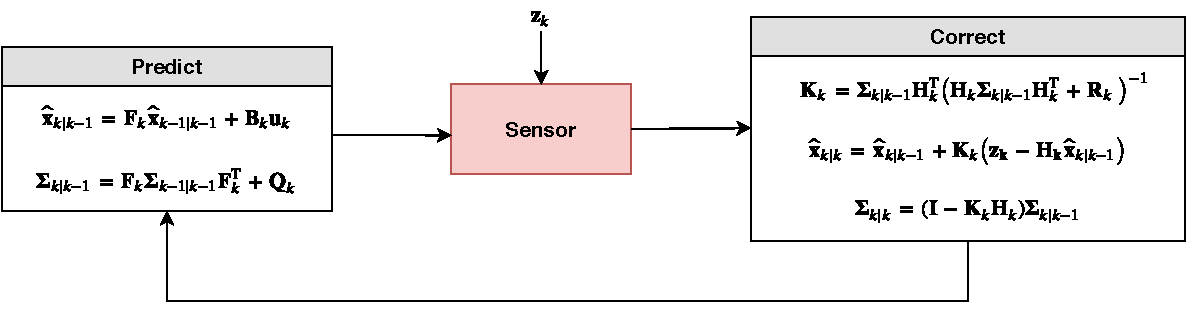
\includegraphics[width=\textwidth]{figures/KF.pdf}
    \caption{The Kalman filtering phases.
    First, \prior state estimate $\xprior$ and error covariance $\priorecov$ are calculated.
    The \prior estimates can be used to control the sensor parameters, that affect observation covariance matrix $\ocov$.
    After the measurement $\z$ has been observed, the \prior estimates can be corrected by utilizing the Kalman gain $\gain$ to get the \post estimates.
    }
    \label{fig:KF}
\end{figure}

Kalman filtering is a Minimum Mean Square Error (MMSE) state estimation algorithm for linear state-space systems \cite{Zarchan2000}.
The discrete-time linear state-space model is expressed using linear combinations as follows \cite{Zarchan2000}
\begin{align}
    \xnext &= \stmodel \x + \cimodel \cinput + \pnoise \label{eq:lsp_state} \\
    \z &= \omodel \x + \onoise \label{eq:lsp_obs}
\end{align}
where $\stmodel$ is state transition matrix, $\cimodel$ is control-input matrix, $ \omodel $ is observation matrix. 
The noise statistics are described with zero mean Gaussian distributions $\pnoise \sim \normal{0}{\pcov}$ and $\onoise \sim \normal{0}{\ocov}$, where $\pcov$ is the process noise covariance matrix and $\ocov$ is the measurement noise covariance matrix.
Kalman filtering is optimal when the state-space model matches the real system, the noises are Gaussian and uncorrelated, and the noise covariances are known \cite{Krishnamurthy2016}.

The Kalman filtering can be divided into two distinct phases as shown in Figure \ref{fig:KF}.
In the first phase, the next state is predicted from the last estimate using expectation of the Equation \eqref{eq:lsp_state}.
The predicted estimates are called \prior estimates, where \prior means predicting next estimates from last estimates without observing a measurement.
On the other hand, \post estimate estimates variable at time instance $k$ when the variable is also observed through the measurements at time instance $k$.
Filtered or \post estimate of the state is obtained at time instance $k$ after observing $\z$ and using the new information in the measurement for correcting the predicted estimate. 
The notation $k|k-1$ is used to denote the \prior estimates and $k|k$ denote \post estimates at time instance $k$.
The \prior error covariance matrix $\priorecov$, which estimates the accuracy of the state estimates $\xprior$, is updated based on the process noise covariance matrix and on the previous estimated \post error covariance matrix.
The prediction phase can be summarized with two equations as follows \cite{Zarchan2000},
\begin{subequations}
\label{eq:kf_predict}
\begin{align}
    \xprior &= \stmodel \xlast + \cimodel \cinput \label{eq:kf_pred_x} \\ 
    \priorecov &= \stmodel \lastecov \stmodel^T + \pcov \label{eq:kf_prior_error_cov},
\end{align}
\end{subequations}
where $\lastecov$ and $\xlast$ are previous \post error covariance matrix and corresponding last \post state estimate.

In the second Kalman filtering phase, a measurement is obtained and the \prior estimates can be corrected using the measurement $\z$ and the Kalman gain $\gain$.
The update phase starts by calculating a residual between the observation $\z$ and the predicted observation $\zhat = \omodel \xprior$.
The residual is called innovation and it is utilized to correct the \prior estimate $\xprior$.
The Kalman gain defines how much the innovation needs to be weighted to correct the predicted estimate $\xprior$.
When the measurement error covariance is high compared to the predicted error covariance, the Kalman gain corrects less the \post estimate compared to situation where measurement error covariance is lower and the measurement can be trusted more. 
The Kalman gain is found by minimizing mean squre error (MSE) between $\x$ and $\xpost$.
As a result, following update equations are obtained
\begin{subequations}
\label{eq:kf_update}
\begin{align}
    \prefitinnov &= \z - \omodel \xprior \label{eq:kf_prefit_innov}\\ 
    \innocov &= \omodel \priorecov \omodel^T + \ocov \label{eq:kf_innov_cov}\\ 
    \gain &= \priorecov \omodel^T \inv{\innocov} \label{eq:kf_gain}\\ 
    \xpost &= \xprior + \gain \prefitinnov \label{eq:kf_update_x}\\ 
    \postecov &= \left( \eye - \gain \omodel \right) \priorecov  \label{eq:kf_post_error_cov}\\
\end{align}
\end{subequations}
where $\innocov$ is the covariance matrix of the innovation $\prefitinnov$. 
Even if the notation in equations \eqref{eq:kf_predict} and \eqref{eq:kf_update} suggests to use \prior or \post estimates on the previous time instance, multiple predictions can be made sequentially or multiple updates can be made at each time interval.

\subsubsection{Interacting Multiple Model estimator}
\label{sec:IMM}

\begin{figure}[b]
    \centering
    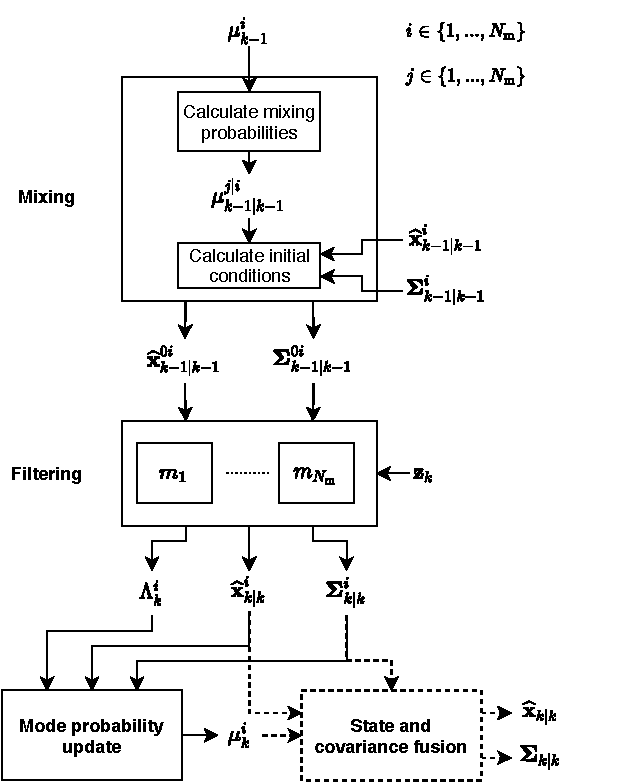
\includegraphics[width=0.7\textwidth]{figures/IMM.pdf}
    \caption{
    The four steps in IMM estimation \cite{BarShalom2001}.}
    \label{fig:IMM}
\end{figure}

In a realistic scenario, the target motion could follow different modes, and the changes between the modes are controlled by an external agent, for example by a human.
Such systems are called hybrid systems. 
They are characterized by a continuous-time stochastic process, such as Equation \eqref{eq:spm_motion}, that describes the motion model for each mode, and by a discrete time stochastic process that describes the evolution of the modes \cite{Mazor1998}.
To clarify terminology, target mode designates specific behavior of a target which is modeled with a target motion model.
Multiple model approach, in which multiple target models are concurrently used for tracking, has emerged for tracking the hybrid systems effectively \cite{BarShalom2001}.
The approach assumes that target motion obeys one of the modes from a finite set of modes at a time.
The underlying mode is identified by a mode matched filter which calculates the probability of each mode given the past observations.
In real-word trackers, the target motion models are chosen to approximate the underlying modes \cite{Simeonova2002}.
For an optimal approach, the number of mode matched filters would grow exponentially in the function of time, even if the modes are switched based on a hidden Markov model (HMM) \cite{BarShalom2001}.
An Interacting Multiple Model (IMM) estimator is a specific suboptimal hybrid filter that achieves a great trade-off between the performance and the computational complexity \cite{Mazor1998}.

An IMM estimator assumes that the target motion at each time instance can be expressed by one of the models infinite set $\mathcal{M} = \{ m_i \}_{i=1}^\nmodels$, where $\nmodels$ is the number of the alternate models.
The switches between the modes are described by an HMM, and the state transition probabilities of the HMM are assumed to be known.
However, in practical scenarios, the modes and the transition probabilities are considered as design parameters \cite{Simeonova2002}.
Given $Z_k$ which is the observation sequence through time $k$, the posterior probability for model $m_i$ to be in effect at time instance $k$ is written as $\Pr{M_k=m_i | Z_k} = \modeprob$, where $M_k$ denotes to model in effect at time instance $k$.

The IMM estimator can be summarized with four steps that are shown in Figure \ref{fig:IMM}.
The steps are mixing, filtering, mode probability update, and state and covariance combination. 
The steps are further implemented as follows.


\begin{description}
% ---------------------------------------------------------
% Mixing
% ---------------------------------------------------------
\item[Mixing.]

Mixing probability is defined as follows
\begin{equation}\label{eq:mixing_conditional_prob}
    \lastmxprobs = \Pr{M_{k-1}=m_j|M_{k}=m_i, Z_{k-1}}.
\end{equation}
which is the probability for a target following mode $m_j$ at time instance $k-1$ if target was following the mode is $m_i$ at time instance $k$ given the observations up to time instance $k-1$.
The equation \eqref{eq:mixing_conditional_prob} can be simplified into form
\begin{equation}
    \lastmxprobs = \frac{1}{\mxnorm} p_{ji} \mu^j_{k-1} \label{eq:imm_mx_probs}
\end{equation}
where $\mxnorm$ is a normalization term, and $p_{ji}$ is the probability of the mode $m_j$ switching to the mode $m_i$. 
The normalization term is defined as follows
\begin{equation}
    \mxnorm = \sum_j^\nmodels p_{ji} \mu^j_{k-1}. \label{eq:imm_mx_normalization}
\end{equation}
The mixing probabilities are used to calculate mixed estimates for the previous posterior state variables and error covariance matrices, which are further used in the tracking filters.
Moreover, the mixed estimates are calculated for the case where it is assumed that the current mode matches to the model $m_i$ of the tracking filter.
Therefore, filtered state and estimation error covariance matrices at time instance $k-1$ are calculated as follows
\begin{subequations}
\begin{align}
    \xmxinit &= \sum_j^\nmodels \lastmxprobs \modexlast \label{eq:imm_mx_init_x}\\
    \ecovmxinit &= \sum_j^\nmodels \lastmxprobs \left[ \modecovlast + \modemxcovlast \right], \label{eq:imm_mx_init_P}
\end{align}
\end{subequations}
where $\modexlast$ and $\modecovlast$ are the last state and covariance posterior estimates of the tracking filter for mode $m_j$, respectively. 
In addition, $\ecovmxinit$ is defined as follows
\begin{equation}
    \modemxcovlast = 
    \left( \xmxinit - \modexlast  \right) 
    \transpose{\left( \xmxinit - \modexlast   \right)}.\label{eq:imm_mx_init_Ptilde}
\end{equation}

% ---------------------------------------------------------
% Filtering
% ---------------------------------------------------------
\item[Filtering.]

In the filtering phase, the likelihood of the observation given the model $m_i \in \mathcal{M}$ is calculated  $\modeobsprob = \Pr{\z | M_k = m_i, Z_{k-1}} $.
The conditioning is approximated by assuming that $\xmxinit$ and $\ecovmxinit$ can be utilized to condition the filters before propagating the filtering equations.
Therefore, the likelihood is obtained from the following relation
\begin{equation}
    \z \sim \normal{\modexprior}{\modeinnovcov},
\end{equation}
where equations \eqref{eq:kf_pred_x} and \eqref{eq:imm_mx_init_x} are used to calculate $\modexprior$, and $\modeinnovcov$ is calculated by using equations \eqref{eq:kf_prior_error_cov}, \eqref{eq:kf_innov_cov}, \eqref{eq:imm_mx_init_P}.

% ---------------------------------------------------------
% Mode probability update
% ---------------------------------------------------------
\item[Mode probability update.]

The mode probabilities $\mu^i_k$ can be updated by using the likelihoods $\Lambda_k^i$ as follows
\begin{equation}
    \mu_k^i = \frac{1}{c} \Lambda^i_k \mxnorm,
\end{equation}
where
\begin{equation}
    c = \sum_{i=1}^\nmodels \Lambda_i^k \mxnorm
\end{equation}
is a normalization constant.

% ---------------------------------------------------------
% State and covariance fusion
% ---------------------------------------------------------
\item[State and covariance fusion.]
Lastly, the posterior estimates $\xpost$ and $\postecov$ can be updated by combining mode probabilities and posterior estimates calculated by each filter.
Thus, the estimates are calculated as follows
\begin{subequations}
\label{eq:imm_estimate}
\begin{equation}\label{eq:imm_fusion_x}
    \xpost = \sum_{i=1}^\nmodels \mu_k^i \modexpost
\end{equation}
\begin{equation}\label{eq:imm_fusion_P}
    \postecov = \sum_{i=1}^\nmodels \mu_k^i 
    \left[ 
        \modecovpost + \left( \modexpost - \xpost \right) \transpose{\left( \modexpost - \xpost \right)}
    \right]
\end{equation}
\end{subequations}
Note that the equations \eqref{eq:imm_estimate} are outputs of the IMM estimator, and not needed for the other IMM estimator steps.
\end{description}


\newpage
\section{Reinforcement Learning} \label{sec:RL}

\begin{figure}[b]
    \centering
    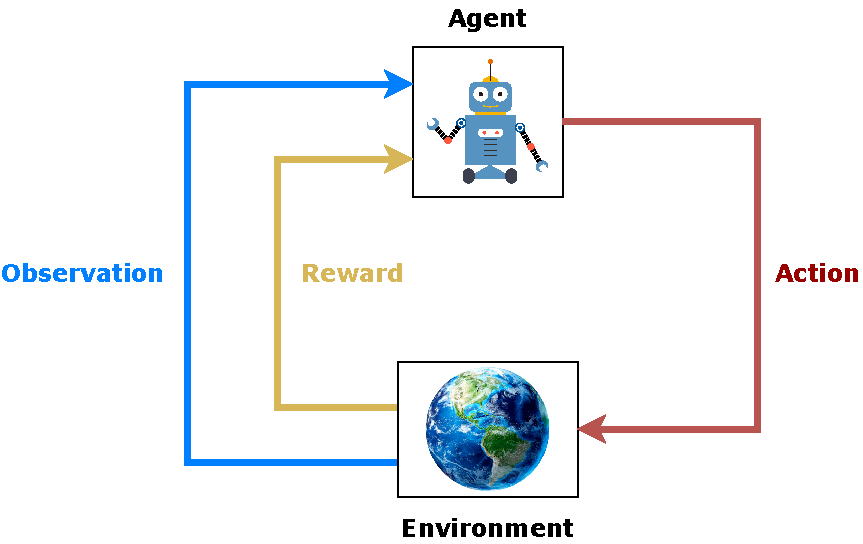
\includegraphics{figures/RL_diagram.pdf}
    \caption{Reinforcement learning.}
    \label{fig:RL_basics}
\end{figure}

Reinforcement learning (RL) is a method for learning to act in stochastic sequential decision-making problems without a model that describe the system dynamics \cite{Sutton2018}.
All RL problems are based on rewards, observations and actions as shown in Figure \ref{fig:RL_basics}.
Thus, identifying the state space, the action space, and the rewards is an essential part of formulating the problem at hand as a reinforcement learning problem.
The learning is based on trial and error approach which is controlled through the reward signal.
The agent independently improves its performance by reasonably probing different actions at for different observations to learn their consequences to the future rewards.

Rewards are defined such that the objective is achieved by maximising sum of future rewards \cite{Sutton2018}.
For example, if an RL method is used to teach a robot to play chess, then positive reward should be given if the robot wins and otherwise no reward is obtained.
Then, the sum of future rewards \eqref{eq:value} indicate the probability of winning given the current state of the game.
In some cases it is more reasonable to use negative rewards.
For instance, if the objective is to minimize the number of steps needed to get out of a maze. 
Then negative reward could be given for each step that emphasizes the agent to learn a policy for taking a minimum amount of steps to get out of the maze.

RL algorithms are based on a Markov decision process (MDP) framework where state transition probabilities and reward distributions are unknown.
This section if organized as follows.
Subsection \ref{sec:MC} introduces a Markov chain which is a fundamental component in an MDP.
Furthermore, MDPs are described in more detail in Subsection \ref{sec:MDP}.
Typical RRM problems are partially observable Markov decision processes (POMDP) in which the MDP state is not fully observable. 
Thus brief introduction to POMDPs are given in in Section \ref{sec:POMDP}.
Finally, in Section \ref{sec:exp_exp} exploration-exploitation dilemma and algorithms to solve it are introduced, and Section \ref{sec:q_learning} introduces Q-learning algorithm which is a particular RL algorithm.


\subsection{Markov chains} \label{sec:MC}

\begin{figure}[b]
    \centering
    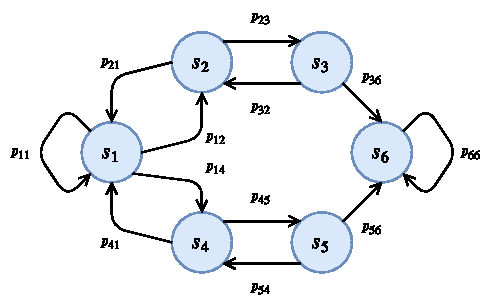
\includegraphics[width=0.8\textwidth]{figures/MarkovChain.pdf}
    \caption{
    An example of a Markov chain with six states. 
    A non-zero state transition probability from state $s_i$ to $s_j$ is written as $p_{ij}$.
    The state transition probability is zero if no arrow exists between a state pair. }
    \label{fig:mc}
\end{figure}


Consider a system that has a finite number of states which describe the operation point of the system.
The set of all different states is denoted by $\Ss$, which is also called state space.
The system state can sequentially transition from state to another state based on a certain stochastic model.
A Markov chain is a stochastic model which can model the sequential state transitions if the transitions are memoryless.
A memoryless transition means that state at time instance $k$, denoted as $S_k \in \Ss$, changes to another state $S_{k+1} \in \Ss$.
Then the following equation will hold   
\begin{equation} \label{eq:markov_property}
    \Pr{S_{k+1} | S_k, S_{k-1}, ..., S_1, S_0} = \Pr{S_{k+1} | S_k}.
\end{equation}
In other words, Equation \eqref{eq:markov_property} indicates that the state transition probability to state $S_{k+1}$ is only dependent on the current state $S_k$.
Thus, there is no need to remember the history of the past state transitions to determine the state transition probability.
The property in Equation \eqref{eq:markov_property} is known as Markov property.

Next, the notation for the Markov chains is clarified.
A Markov chain has $\nstates$ states which are represented as $s_i \in \{s_1, s_2, ..., s_{\nstates} \}$.
If state is a random variable, it is denoted by $S_k$ where $k$ is the time index.
For example, $S_k = s_i$ means that the state at time instance $k$ is realized as $s_i \in \Ss$. 
The state transition probability from state $s_i$ to state $s_j$ is defined as $\Pr{S_{k+1}=s_j | S_{k}=s_i}=p_{ij}$.
Moreover, it is possible to summarize the Markov chain dynamics with a state transition matrix $\stprobs$ in which the element on row $i$ and column $j$ corresponds to the probability $p_{ij}$.
An example of a Markov chain with six states is shown in Figure \ref{fig:mc}.

\subsection{Markov decision process} \label{sec:MDP}

\begin{figure}
    \centering
    \begin{subfigure}[b]{0.45\textwidth}
        \centering
        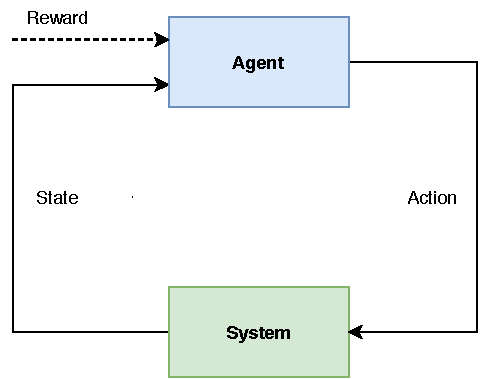
\includegraphics[width=0.9\textwidth]{figures/MDP.pdf}
        \caption{
        In an MDP, the agent takes an action that interacts with the system.
        After the action is taken, the agent receives a reward and a new state of the system.
        The reward can be dependent on the action and the state transition.
        The new system state is used to decide the next action.}
        \label{fig:mdp}
    \end{subfigure}
    \hfill
    \begin{subfigure}[b]{0.45\textwidth}
        \centering
        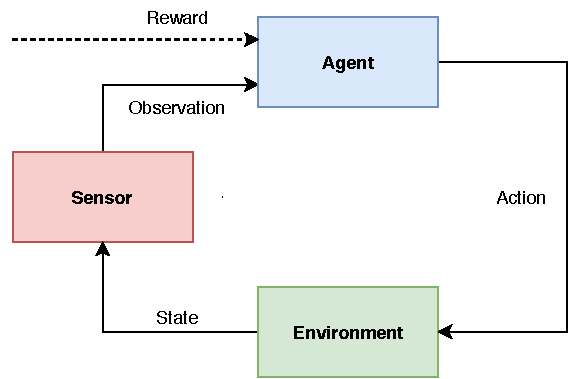
\includegraphics[width=\textwidth]{figures/POMDP.pdf}
        \caption{
        A POMDP is an extended MDP where the system state is observed through a sensor.
        The sensor can be for example a radar, and the measurements provide noisy and partial state of the system. 
        In comparison to the MDP, the reward function can be additionally dependent on the observations.
        }
        \label{fig:pomdp}
    \end{subfigure}
    \caption{Markov decision process (MDP) and partially observable Markov decision process (POMDP) visualized. }
    \label{fig:MDP_and_POMDP}
\end{figure}

A sequential decision process is a process where a decision-maker needs to sequentially make decisions that affect future decisions \cite{LaValle2006}.
If the outcomes of the decisions are non-deterministic, then the decision process is considered as a stochastic sequential decision process.
A Markov decision process (MDP) is a mathematical framework that is used to formalize stochastic sequential decision-making problems \cite{Sutton2018}.
The decision-maker in an MDP is called an agent.

The key element of an MDP is that the system is modeled as a Markov chain.
The agent observes the current state $s \in \Ss$ and chooses an action $a$ from a set of possible actions $\As$, which is also known as the action space.
In some cases, the possible actions are dependent on the current state.
Therefore, state-specific action space is denoted as $\As_s \subseteq \As$, which used to emphasize the coupling between state $s$ and the available actions. 
The action activates a state transition of the Markov chain, and the state transition probabilities $\stprobs$ can be dependent on the action.
The action dependent state transition probability for $s$, $s' \in \Ss$ and $a \in \As$ is denoted by 
\begin{equation}\label{eq:mdp_st_prob}
    \mathrm{T}(s, s', a) = \Pr{S_{k+1}=s' | S_{k}=s , A_k=a}
\end{equation}
where $A_k$ is the action taken at time instance $k$.  
After the state transition, the agent receives a scalar reward.
The reward can be stochastic and the reward distribution can be dependent on which action was taken and on the state transition.
The set of all possible rewards is a subset of real numbers $\Rs \subseteq \real$, and the subset $\Rs_{ss'}^a \subseteq \Rs$ is the set of state transition and action dependent rewards.
The dynamics of an MDP can be summarized with a single probability distribution
\begin{equation}\label{eq:MDP_probs}
    p(s', r | s, a) = \Pr{ S_{k+1}=s', R_{k+1}=r | S_k=s, A_k=a }.
\end{equation}
which is the probability that system changes from state $s \in \Ss$ to state $s' \in \Ss$ after the action $a \in \As_s$ was taken and agent receives immediate reward $r \in \Rs_{ss'}^a$ at time instance $k+1$.

An MDP can last for a finite or infinite number of steps, and the number of the steps is called horizon.
The objective of the agent is to maximize the sum of rewards on the given horizon.
In an infinite horizon MDPs, the agent desires to maximize the sum of discounted future rewards.
The sum of future rewards discounted with a discount factor $0 \leq \lambda < 1$ is defined as
\begin{equation}\label{eq:discounted_sum}
    G_k = \sum_{i=0}^{\infty} \lambda^i R_{k + i + 1}
\end{equation}
where $R_{t+k+1}$ is the reward received from taking action $A_{t+k}$. 
From the perspective of RL, theory for infinite horizon MDPs is more important \cite{Sutton2018}, thus rest of the chapter will concentrate on infinite horizon MDPs.

In MDP it is assumed that the system state $S_k \in \Ss$ can be observed at each time instance $k$.
Therefore, the agent needs to find a policy $\pi(a | s)$ which gives the probability for taking action $a \in \As$ given the state $s \in \Ss$.
The optimal policy is defined as
\begin{equation}\label{eq:mdp_optimal_policy}
    \pi^* = \arg\max_\pi\Epolicy{G_k | S_0}.
\end{equation}
which is the policy that achieves the greatest expected discounted sum of rewards.
By the definitions \eqref{eq:discounted_sum} and \eqref{eq:mdp_optimal_policy}, the optimal policy would need to consider all the future actions.
Such policies are called non-myopic policies.
In comparison, a policy where the agent maximizes the immediate reward is called a myopic policy. 
Typically, the myopic policies are suboptimal for $\lambda>0$.

Since an optimal policy maximizes the discounted sum of expected future rewards, a reasonable way to evaluate policy $\pi$ is to calculate value of state $s \in \Ss$ using the following equation
\begin{equation} \label{eq:value}
    v_\pi(s) = \Epolicy{G_k | S_k=s},
\end{equation}
where the function $v_\pi(s)$ is called value function \cite{Sutton2018}.
The value function gives the expectation of the discounted rewards given the initial state $s$ and the policy $\pi$.
Moreover, the optimal policy $\pi^*$ has always greater or equal value for any state $s \in \Ss$ compared to any other policy $\pi$.
Similarly, another function that can measure the quality of any action $a \in \As$ given the state $s \in \Ss$ is defined as
\begin{equation}\label{eq:action_value}
    q_\pi(s, a) = \Epolicy{G_k | S_k=s, A_k=a},
\end{equation}
and it is called an action-value function.
It can be noted that the value function $v_\pi(s)$ and the action-value function $ q_\pi(s, a)$ are connected to each other through the equation  
\begin{equation}\label{eq:value_action_value}
 v_\pi(s) =  \sum_{a\in \As_s} \pi(a | s) q_\pi(s, a),
\end{equation}
in which the action-values are weighted by the probabilities of choosing the action.

Lastly, it is quite straightforward to prove that the value function \eqref{eq:value} can be expressed in a recursive form 
\begin{align}
    v_\pi(s) 
    &= \Epolicy{ \sum_{i=0}^{\infty} \lambda^i R_{k + i + 1} | S_k=s} \\
    &= \Epolicy{R_{k + 1} + \lambda \sum_{i=0}^{\infty} \lambda^i R_{k + i + 2} | S_k=s} \\
    &= \sum_{a \in \As_s} \pi(a | s) \sum_{s' \in \Ss} \sum_{r \in \Rs_{ss'}^a} p(s', r | s, a) \left[ r + \lambda v_\pi(s') \right]\label{eq:bellman},
\end{align}
where \eqref{eq:bellman} is called Bellman equation \cite{Sutton2018}.
Similarly, the Bellman equation for action-values can be expressed as follows
\begin{equation}\label{eq:bellman_action}
     q_\pi(s, a) = \sum_{s' \in \Ss} \sum_{r \in \Rs_{ss'}^a} p(s', r | s, a) \left[ r + \lambda v_\pi(s') \right],
\end{equation}
which is conducted from equation \eqref{eq:bellman} using the equation \eqref{eq:value_action_value}.
The Bellman equation is the key for solving MDPs because it enables using recursion to calculate the values \eqref{eq:value} or action-values \eqref{eq:action_value} for example in the case of dynamic programming.


\subsection{Partially observable Markov decision process} \label{sec:POMDP}


A partially observable Markov decision process (POMDP) is an extension to the MDP framework. 
The difference between an MDP and a POMDP is that the state of a Markov chain is not fully observable \cite{Krishnamurthy2016}.
A Markov chain that is not fully observable is called a hidden Markov model (HMM).
In real-world systems, state of a Markov chain is usually partially observable because sensor measurements contain random noise that is unobservable or the observation does not contain the full information about the state.

The POMDP framework extends the MDP framework by introducing observation space $\Os$ which is set of all possible observations.
An observation $z \in \Os$ is connected to state $s' \in \Ss$ and action $a \in \As$ by the observation probability
\begin{equation}\label{eq:pomdp_obs_prob}
    \Op(z , s', a) = \Pr{Z_{k+1}=z | S_{k+1}=s', A_k=a},
\end{equation}
which indicates that the probability of observing $z$ at time instance $k+1$ is conditional to the action $a$ taken at time instance $k$ and state of the system $s'$ at time instance $k+1$.
Thus, instead of observing the full state $S_{k+1}$ after an action, the agent obtains an observation which is conditioned on the full state.
From Equation \eqref{eq:mdp_st_prob} and Equation \eqref{eq:pomdp_obs_prob}, it can be seen that in POMDP problem, the action can affect both observation and state transition probabilities.

Generally, a policy that is used to address a POMDP problem is dependent on the complete history of past actions and observations. 
The history is called the information history.
The information history until time instance $k$ is written as $I_k=\{A_0, Z_1, A_1, Z_2, ..., A_{k-1}, Z_{k}\}$, where $A_k \in \As$ and $Z_k \in \Os$ are the action and the observation at time instance $k$, respectively.
It is possible to utilize the information history $I_k$ to calculate the probability
\begin{equation}
    b_k(s) = \Pr{S_k=s|I_k}
\end{equation}
which is the probability of a Markov chain being on a state $s$ given the information history.
At each time instance $k$, the probabilities can be calculated for each state $s \in \Ss$, which is denoted as the belief state $b$.
After taking action $a \in \As$ and observing observation $z \in \Os$, the belief state can be updated by Bayesian update rule \cite{Krishnamurthy2016}
\begin{align}
    b_{k+1}(s') 
    &= \Pr{S_{k+1}=s' | Z_{k+1}=z, A_k=a, I_k} \\
    &= \frac
        {\Pr{Z_{k+1}=z | S_{k+1}=s' , A_k=a, I_k} \Pr{S_{k+1}=s'| A_k=a, I_k}}
        {\Pr{Z_{k+1}=z | A_k=a, I_k}} \\
    &= \frac
        {\Op(z, s', a) \sum_{s \in \Ss} \mathrm{T}(s, s', a) b_k(s)}
        {\sum_{s''  \in \Ss} \left[ 
            \Op(z, s'', a) \sum_{s \in \Ss} \mathrm{T}(s, s'', a) b_k(s) \right]}  \label{eq:belief_state_update}
\end{align}
which can be used to calculate belief probabilities for each state $s' \in \Ss$.

The number of belief states is infinite since the probabilities $b_k(s)$ are continuous.
An approach to solve a POMDP is to formulate the problem as a continuous state MDP where the belief state $b$ is used as a state variable instead of using the state variable $s$.
Thus, the policy can be written as $\pi(a | b)$, which is the probability of choosing the action $a$ given the belief state $b$.

\subsection{Exploration and exploitation}\label{sec:exp_exp}

Exploration and exploitation are essential concepts in RL. 
They allow for the RL agent to improve the policy by simple trial-and-error method.
Initially, the agent starts with no knowledge about the system dynamics meaning that the initial policy may be random.
Therefore, the agent needs to utilize a policy for probing different actions that have unknown consequences.
The probing is used to gain more knowledge about the dynamics, and the increased knowledge can be utilized to improve the policy.
The actions that are taken to gain more knowledge are called exploration actions.
Otherwise, the agent is exploiting, which means that the agent chooses the action that is currently believed to be the best action.
The dilemma of finding the balance between exploration and exploitation is called exploitation-exploitation trade-off.

Widely used policy for balancing the exploration-exploitation trade-off is called \egreedy policy \cite{Sutton2018}.
With \egreedy policy, the agent chooses random action with probability $\epsilon$.
When not choosing the action randomly, the action with highest action-value is selected.
Therefore, the policy can be written as follows
\begin{equation}\label{eq:epsilon_greedy}
    a =
    \left\{
        \begin{array}{ll}
            \arg\max_{a' \in \As} q_\pi(s, a') & \text{with probability $1-\epsilon$}\\
            \text{random action} & \text{with probability $\epsilon$}.
        \end{array}
    \right.
\end{equation}
where $a$ is the chosen action and $0 < \epsilon \ll 1$.

With fixed exploration parameter $\epsilon$, the optimality cannot be achieved since random actions will be always taken.
One solution is to gradually decay the parameter $\epsilon$, but specifying the decay rate can be tedious without causing a significant change in the convergence speed.
Majority of the other exploration and exploitation policies that have been proposed in the literature are not suitable for solving general RL problems \cite{Slivkins2019}.
Instead, they are suitable for a particular RL problem called stochastic multi-armed bandit (MAB) which is an MDP with one state.

\subsubsection{Stochastic multi-armed bandits}\label{sec:MAB}

The stochastic MAB problem is a sequential decision-making problem in which an agent needs to choose an action among several competing actions \cite{Sutton2018}.
The word arm originates from a slot machine that has a pull lever, and the pull lever is called an arm.
Pulling an arm of a slot gives a reward based on a certain probability distribution.
In the MAB problem, the agent needs to sequentially decide from many arms which arm to pull to maximize the cumulative reward.
The strategy of how the agent chooses the arms is called a policy.
The stochastic MAB problem is a MDP with one state \cite{Sutton2018}.
It is different from Markovian MAB problem in which each machine is modeled with a Markov chain \cite{Katehakis1987}.


Usually, the performance of a policy is measured with regret.
The regret quantifies the cost of learning by measuring how much reward agent has missed from the optimal cumulative reward.
The regret is defined as follows
\begin{equation}\label{eq:basic_reg}
    L_\pi(K) = \sum_{k=1}^T \mu^*_k - \mu^\pi_k,
\end{equation}
where $K$ is the time horizon, $\mu^\pi_k$ is the expected reward for the policy $\pi$ at time instant $k$, and $\mu_k^*$ is the expected reward for the optimal arm at time instant $k$.

This thesis utilizes the following criterion
\begin{equation}\label{eq:reg}
    L_\pi(T) = \sum_{t=1}^T \frac{\mu^*_t - \mu^\pi_t}{\mu^*_t},
\end{equation}
in which the missed rewards from the optimum rewards are normalized with the maximum rewards.
The equation \eqref{eq:reg} is referred as normalized regret.
The normalized regret describes how large proportion of the optimal reward is missed at each time instance, which is useful when the rewards are non-stationary.

To maximize the cumulative reward, the agent needs to find the arm which gives the highest expected reward.
This means that the agent needs to decide when to explore different arms to possibly identify those with higher expected rewards 
and when to keep pulling the arm with currently known highest expected reward.
An estimate for the expected reward is updated each time when the agent has pulled an arm.
The update equation for each arm can be written as
\begin{equation}\label{eq:update1}
    q_{k+1}(a) = q_{k}(a) + \alpha \left(R_{k+1} + q_{k}(a)\right),
\end{equation}
where $R_{k+1}$ is the received reward from selecting the arm $a$, $\alpha$ is a step size and $q_{t}(a)$ is called an action-value \cite{Sutton2018}.
For stationary rewards, $\alpha$ can be set to $t^{-1}$, so that (\ref{eq:update1}) calculates the empirical mean. 
For non-stationary rewards, the parameter $\alpha$ needs to be constant so that old rewards have a lower weight than more recent ones \cite{Sutton2018}.

In practice, a policy is realized as an algorithm.
Five commonly used MAB algorithms are reviewed here, because the algorithms are widely used to solve MAB problem and used for simulations in Chapter \ref{sec:RL_TX_RX}.
These algorithms are
\begin{enumerate}
    \item $\epsilon$-greedy \cite{Lattimore2019},
    \item Upper Confidence Bound (UCB1) \cite{Auer2002, Aurelien2008},
    \item Kullback Leibler Upper Confidence Bound (KL-UCB) \cite{Garivier2011},
    \item Thompson sampling \cite{Agrawal2012, Raj2017}, and
    \item Recency-Based Exploration (RBE) \cite{Oksanen2015,Oksanen2017}.
\end{enumerate}
The \egreedy algorithm was already given in Equation \eqref{eq:epsilon_greedy}, but the states are not needed to consider in the stochastic MAB problem.
Thus, \egreedy algorithm chooses random arm with probability $\epsilon$ which remains constant or decreases slowly in time. 
When not selecting an arm randomly, the algorithm chooses the arm which has the highest action-value.
UCB1, KL-UCB, Thompson sampling and RBE algorithms are index-based polices that calculate a quantity, called an index, for each arm.
The index captures the uncertainty on the action-value $q_t(a)$ and emphasizes exploration for those arms that might have desirable expected rewards.
The index is constructed in a way that the arm with highest index is selected as follows

The UCB1 and KL-UCB are policies are based on deriving an upper confidence bound for the expected rewards and the arm with highest bound is selected \cite{Sutton2018, Garivier2011}.
To ensure asymptotic optimality, the bound is tighten in function of time.
For example, the UCB1-algorithm selects the arm as follows \cite{Auer2002}
\begin{equation}
    A_k = \argmax_{a \in \As} q_k(a) + \sqrt{\frac{2 \ln{k}}{\#_a(k-1)}},
\end{equation}
where $k$ is the time index, and $\#_a(k-1)$ denotes the number of times arm $a \in \As$ is chosen at time instance $k-1$.
The UCB1-algorithm is guaranteed to achieve logarithmic regret for $R_t \in [0, 1]$ as shown in \cite{Auer2002}.
Sublinear regret indicates that the agent has made choices in previous time instances that improve the future choices.
The KL-UCB algorithm improves regret bounds by utilizing Kullback-Leibler divergence between the expected arm distributions and upper bounded distributions \cite{Garivier2011}.
However, it requires more computationally involved optimization step to obtain the upper bound.

Thompson sampling is a Bayesian algorithm where the posterior probability distributions for the expected rewards are formed from the collected rewards \cite{Agrawal2012}.
Then the posterior distributions are sampled at each time instant and the arm with the highest sample is selected.
Finally, the RBE is based on defining an exploration bonus to support choosing arms which have not been explored recently \cite{Oksanen2015}
In addition, the index is constructed in a way that the agent prefers arms which have the highest action-values.
Thus, the arm is selected as follows
\begin{equation}
    A_k = \argmax_{a \in \As} q_k(a) + \sqrt{2\ln{\frac{k}{\tau_k(a)}}},
\end{equation}
where $\tau_k(a)$ is the last time index when the arm $a$ was previously selected. 


\subsection{Q-learning algorithm}\label{sec:q_learning}

\begin{algorithm}[htb]
    \SetAlgoLined
    Initialize $Q(s, a) \forall s \in \Ss, a \in \As$\;
    \While{\text{learning}}{
    choose $a$ using policy $\pi$ ($\argmax_a Q(s, a)$ and $\epsilon$-greedy)\;
    $r, s' \leftarrow$ take action $a$\;
    $Q(s, a) \leftarrow Q(s, a) + \alpha (r + \lambda \max_a Q(s', a) - Q(s, a))$\; 
    }
\caption{Q-learning algorithm with \egreedy exploration \cite{Sutton2018}}
\label{alg:q_learning}
\end{algorithm}

This section introduces Q-learning algorithm which is widely known algorithm in RL literature. 
The algorithm is based on a temporal-difference (TD) learning, which utilizes DP and Monte Carlo method. 
The Monte Carlo method refers to an approach that obtains the values $V(s)$ or action-values $q(s, a)$ by sampling and calculating empirical mean from the obtained samples. 
It is similar to method which was introduced in Section \ref{sec:MAB}, where expected rewards of the arms were calculated using the update rule in Equation \eqref{eq:update1}. 
Whereas, the Monte Carlo methods utilize the same principle in general RL problems, in which the discounted sum of rewards is maximized. 
The following equation 
\begin{equation}\label{eq:update_mc}
    Q(s, a) = Q(s, a) + \alpha (G_t - Q(s, a))
\end{equation}
is used to update the action-values of a given policy with a Monte-Carlo method. 
It is required to run the whole episode in order to get the discounted sum $G_t$.
For infinite horizon MDPs the episode can be replaced by running the algorithm for sufficient number of future states.
However, the recursion in the Bellman equation \eqref{eq:bellman_action} can be further utilized to rewrite Equation \eqref{eq:update_mc} as follows 
\begin{equation}\label{eq:update_td}
    Q(s, a) = Q(s, a) + \alpha \left( r + Q(s', a') - Q(s, a) \right)
\end{equation}
where the discounted sum $G_t$ is replaced with recursive form.
Moreover, $Q(s', a')$ is bootstrapped by using the value that is current Q-value for action $a'$ and $s'$ when following a certain policy.
The parameter $\alpha$ cannot be $\frac{1}{k}$ to calculate the empirical mean, as it could be in Monte-Carlo method, because $Q(s', a')$ values are non-stationary.
The advantage of using TD learning compared to Monte Carlo method is that the Q-values can be updated at each time instance, instead of waiting until end of an episode.

In general case, the RL policy can be divided into target and behavior policies \cite{Sutton2018}.
The behavior policy is used to improve the target policy which is usually better in terms of achieving higher rewards.
Off-policy RL algorithms have different behavior and target policies.
Typically, behavior policy implements the exploration-exploitation trade-off which is required to converge to an optimal policy. 
In addition, the target policy is typically purely for exploitation. 
On-policy RL algorithms do not have separate behavior and target policies. 

Q-learning is a specific off-policy TD learning algorithm. 
The algorithm updates its action values using Equation \eqref{eq:update_td}, where the next action value is estimated by using a target policy, 
and behavior policy is used to select an action while learning. 
The target policy selects the action with the highest action-value.
Typical choice for behavior policy is the epsilon-greedy policy. 
The target policy learns directly the optimal Q-values regardless of the behavior policy. 
The Q-learning algorithm with epsilon greedy policy is shown in Algorithm \ref{alg:q_learning}.

To apply Q-learning for continuous or large state spaces, function approximators have been employed to approximate the action-value function \cite{Sutton2018}. 
Especially, deep neural networks have been widely adopted to solve RL problems with continuous state spaces in different application domains \cite{Mnih2013, Zhang2018, Luong2018}.
However, the training required to train deep RL agent can get quite intensive \cite{Irpan2018}.
For RL problems that involve neural networks, the models are usually trained with simulations and then fine-tuned in the real environment.


\clearpage
\section{Radar Resource Management} \label{sec:existing_RRM}


Phased-array technology has enabled modern radars to carry out multiple radar functions simultaneously, including target tracking, and search for undetected targets.
Each radar function executes one or more tasks and each radar task may involve multiple looks.
For example, a radar task can indicate tracking a specific target, and maintaining the task may require multiple looks.
Look of a radar is defined to be uninterruptible and have finite duration in which radar beam is steered into one or more positions \cite{Moo2016}.
Scheduler is responsible for deciding when each look is executed, and which looks are dropped in overload situations \cite{Moo2016}. 
Task prioritization is used to emphasize scheduler to prefer tasks with high priority over low priority to solve overload situations where all of the tasks cannot be executed simultaneously.
Radar Resource Management (RRM) considers scheduling of the radar looks, prioritization of the radar tasks as well as allocating radar resources and selecting operational parameters \cite{Moo2016}. 

For monostatic and bistatic radars, three major resources include time, processing, and energy resources. 
Multistatic radars have an additional degree of freedom to allocate and configure individual radars for the radar tasks \cite{Moo2016}. 
Moreover, cognitive radars use the perception-action cycle to exploit past observations and constructed situational awareness for improved performance in the future \cite{Haykin2006}. 
Thus, the perception-action cycle creates an additional source of information to be used for RRM.
An efficient RRM is required to maximize the radar resource utilization for optimal behavior which is quantified by utility functions. 

Operational parameters of a radar are optimized or selected for a given look to maximize utility functions. 
Modern radars can adaptively select almost any radar operational parameter such as transmit power, frequency, bandwidth, revisit interval, dwell time and PRF as well as to choose among different waveforms.
In addition, radar networks such as distributed MIMO radars can select different TX and RX configurations \cite{Godrich2011a, Godrich2011, Sun2014}.
Radar networks create additional difficulty in RRM because each radar can be configured and scheduled individually to improve the overall performance \cite{Sun2014}.

Time Budget Management (TBM) is a subproblem of RRM in which radar time resources are allocated for radar looks and the looks are scheduled into the timeline. 
The time duration of the look is called dwell time, and the time duration between the looks for a given task is called revisit interval (RI). 
The dwell times and RIs are illustrated in Figure \ref{fig:timeline}. 
If a tracking task is considered, the RI is the time between the track update trials. 
The time budget of a multifunction radar is shared among multiple functions such as tracking, searching and classification.
If multiple tasks can be executed by a functional subsystem or a complete radar set, then the TBM problem is considered to have multiple channels \cite{Shaghaghi2018}.
However, in this thesis the focus is on single channel TBM problems.
Considerably many approaches solve the TBM as a subproblem of general RRM problem, including \cite{Koch1999, Wintenby2006, Byrne2016, Xu2010}. 
However, in \cite{Rajkumar1997, Irci2010, Charlish2015a} the TBM management is implemented jointly along with allocating other radar resources and while optimizing the operational parameters of the radar.


In the following sections, general radar RRM problem is considered in more detail, and two specific RRM subproblems are described.
Section \ref{sec:RRM_tech} presents classification of RRM techniques to understand higher level solutions for RRM problems.
Section \ref{sec:TX_RX_selection_review} considers the TX-RX selection problem for distributed MIMO radars. 
In Section \ref{sec:tbm_ri}, revisit interval selection (RIS) problem is considered which is related to the TBM problem.


\begin{figure}[h]
    \centering
    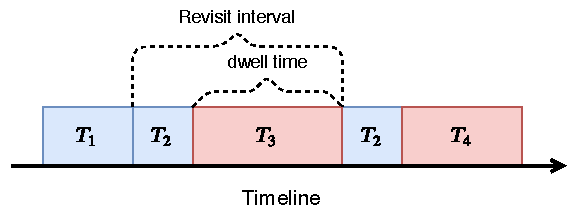
\includegraphics{figures/timeline.pdf}
    \caption{
        The looks for the tasks $T_i \forall i\in\{1,2,3,4\}$ are scheduled on a radar timeline. 
        The revisit interval and the dwell time of the looks are illustrated.
        The blue and red colors are used to indicate tasks corresponding to different radar functions such as tracking and search functions.
    }
    \label{fig:timeline}
\end{figure}

\subsection{Radar Resource Management techniques} \label{sec:RRM_tech}

\begin{figure}[tb]
    \centering
    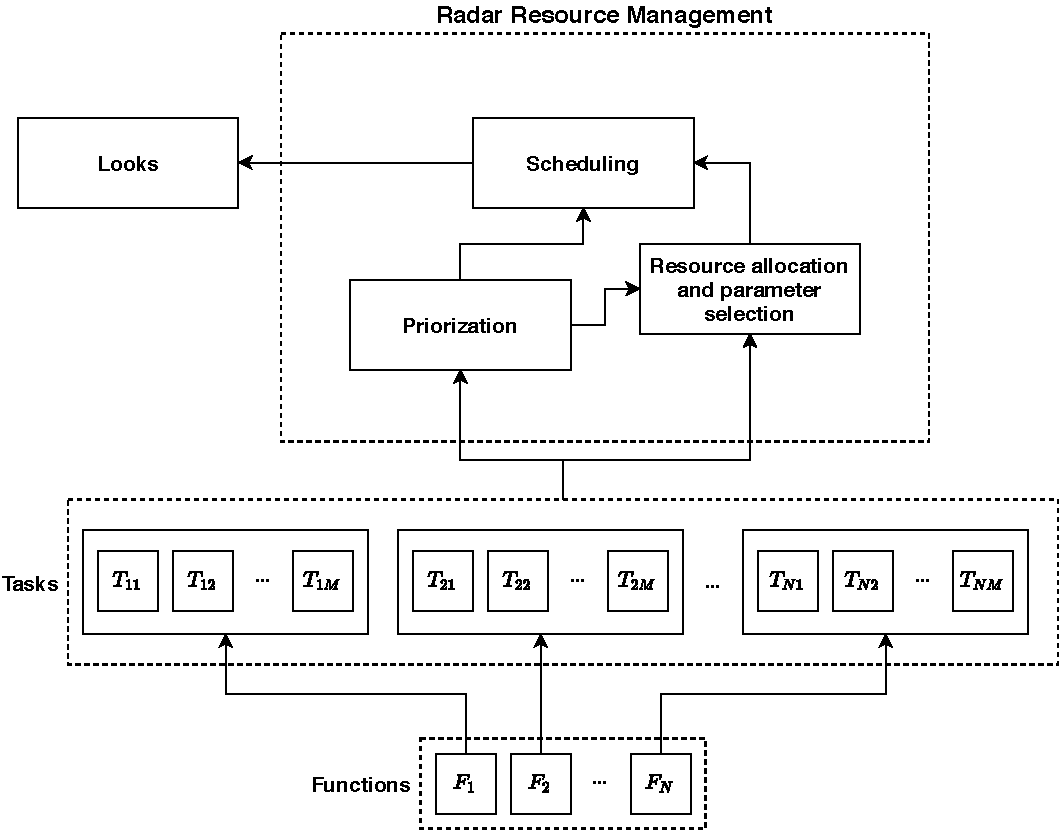
\includegraphics[width=.9\linewidth]{figures/RRM_diagram.pdf}
    \caption{Typical components in Radar Resource Management (RRM).}
    \label{fig:RRM_diagram}
\end{figure}

Typical RRM algorithms can be divided into three components that prioritize, allocate and schedule radar resources as shown in Figure \ref{fig:RRM_diagram}.
However, for some RRM techniques the division is not strict.
For example, RRM techniques can implement the functions of each aforementioned component jointly while optimizing the objective function.
The following techniques for addressing RRM problems were identified from the literature \cite{Moo2016, Koch1999, Krishnamurthy1999, Krishnamurthy2001, Wintenby2006, LaScala2006, Rajkumar1997, Rajkumar1998, Kastella1997, Kreucher2004, Kreucher2005, Xu2010}.

\begin{description}

\item[Rule-based approach.]

Rule-based RRM include approaches in which local objective is optimized instead of optimizing the global objective \cite{Koch1999}.
Alternatively, the parameters are fixed such that the radar resource manager is not fully exploiting the degrees of freedom of the modern radars.
Significant research direction in rule-based approaches is developing adaptive RIS algorithms \cite{Cohen1986, Gardner1988, Munu1992, ChengTing2007, Baek2010, Watson1993, Charlish2015, Keuk1975, Shin1995, Benoudnine2006}. Those algorithms will be covered in more detail in Section \ref{sec:tbm_ri}.


\item[Stochastic dynamic programming.]

Stochastic Dynamic Programming (SDP) is a generalized framework for solving decision-making problems under uncertainty. 
The  Markov Decision Process (MDP) is a special case of SDP for which the Markov property is fulfilled and states and actions are discrete.
The RRM problem can be interpreted as a decision-making problem in which the decision-maker needs to decide when to execute the radar looks, and how much radar resources are allocated for them \cite{Krishnamurthy1999, Krishnamurthy2001, Wintenby2006, LaScala2006}.
Important characteristic of the SDP approach is that the decisions are made to account long-term consequences.
However, the optimal solution is unfeasible with realistic assumptions \cite{Wintenby2006}.
Therefore, the RRM is relaxed to two time-scale RRM problem where SDP is used to solve slow-time-scale (STS) optimization problem and low-level scheduler is used to solve fast-time-scale (FTS) scheduling problem \cite{Wintenby2006}.  


\item[Quality of service resource allocation model.] 

Quality of service Resource Allocation Model (Q-RAM) was initially proposed in \cite{Rajkumar1997}.
Q-RAM algorithms optimize global utility function while satisfying the resource constraints.
Thus, the approach is different from the rule-based RRM techniques in which local objectives are optimized.
Q-RAM addresses the resource allocation problem in which resources are allocated for the radar looks, but the actual order of the looks is not considered.
However, the schedulability requirement ensures that the the looks can be scheduled when using a given low-level scheduling algorithm. 
In general, the Q-RAM optimization problem is unfeasible, but practical approximation algorithms are proposed in \cite{Rajkumar1998, Irci2010, Charlish2015a}.

\item[Information-theoretic approach.]

In the information-theoretic approach, surveillance area is divided into smaller grid cells \cite{Kastella1997, Kreucher2004, Kreucher2005, Xu2010}.
Probability of target existing in a given grid cell is calculated based on prior probabilities and past observations.
Information theoretic measure is used to calculate the obtained utility from taking different actions i.e. observing certain cells or selecting different waveforms.
Thus, the information theoretic approach does not differentiate search and tracking tasks since its purpose is to minimizes uncertainty in the surveillance area.

\end{description}


\noindent
The RRM algorithms can have characteristics from multiple technique classes. 
For example, in \cite{Byrne2015, Byrne2016} the objective function is similar to Q-RAM approach as well as the objective considers long-term consequences as in SDP approaches.
Additionally, in \cite{Esfahani2012} locally optimized QoS parameters are utilized in allocating radar time budget to optimize global objective using a heuristic algorithm.

\subsection{Distributed MIMO radar transmitter-receiver selection}\label{sec:TX_RX_selection_review}

\begin{figure}[b]
    \centering
    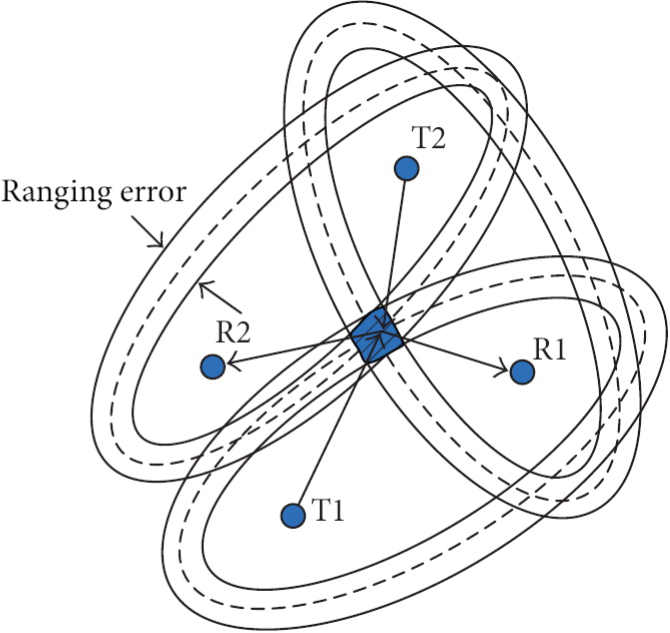
\includegraphics[width=0.5\textwidth]{figures/background/MIMO_TX_RX_selection.png}
    \caption{Target localization with distributed MIMO radar. Reprinted from \cite{Sun2014}.}
    \label{fig:dist_MIMO_localization}
\end{figure}


In distributed MIMO radars, the increased number of channels provide additional spatial diversity and degrees of freedom at the cost of larger amounts of data to be processed and higher power consumption \cite{Haimovich2008}.
In addition, active TXs may expose their location which might be undesired in certain applications.
Strategies for TX-RX subset selection are studied to obtain desired spatial diversity gain, and to reduce the cost and the power consumption at the same time.

In \cite{Godrich2011a, Godrich2011}, the subset selection was formulated as a Knapsack
Problem (KP) which is a specific combinatorial optimization problem.
In the KP, each item in a given set of items are associated with a weight and a value, and the objective is to select such items that the total value is maximized while total weight is below a certain limit.
Moreover, in the considered KP formulations, the items were associated with costs instead of values such that total costs were minimized.
An item in the TX-RX subset selection problem is either TX or RX.

The KP in \cite{Godrich2011a} was formulated for minimal subset selection, in which minimal number of TXs and RXs are selected with a required target localization accuracy.
In other words, the weight is related to the target localization uncertainty associated with the subset, and the cost was the operational cost involved with using additional TX or RX.
In \cite{Godrich2011} the KP was formulated for K-subset selection, in which the number of TXs and RXs in the subset is equal to $K$.
Therefore, the weight for each TX or RX is one, and the total weight is required to be less than $K$.
In addition, the cost was based on the target localization uncertainty.

The TX-RX subset selection strategies proposed in the literature utilize target localization accuracy related performance criteria \cite{Godrich2011a, Godrich2011, Sun2014}.
The target localization accuracy is dependent on the geometry of distributed MIMO radar layout as depicted in Figure \ref{fig:dist_MIMO_localization}.
In \cite{Godrich2011a, Godrich2011}, Cram\`er-Rao bound (CRB) was derived for the target position estimate, and a trace of the CRB was used as a performance criterion.
The trace of CRB is related to Geometric Dilution Of Precision (GDOP) which is commonly used measure in Global Positioning Systems (GPS) \cite{Sun2014}. 
A criterion based on information theoretic was proposed in \cite{Sun2014}.
The metric is called Fisher Information Distance (FID) which calculates similarity of probability distributions for position estimate between using the TX-RX subset and all TXs and RXs.
The benefit of using FID is its ability to measure how close the subset performance is compared to the case where all TXs and RXs are selected \cite{Sun2014}.

There are multiple ways to solve the aforementioned KPs.
The simplest approach is to use exhaustive search as in \cite{Sun2014}.
However, the number of subsets grow exponentially as a function of the number of TXs and RXs.
Therefore, solving the problem may become intractable in case of larger MIMO radar configurations.
In order to solve such a problem, heuristic approximation algorithms are proposed in \cite{Godrich2011a, Godrich2011} to optimize the KPs.
The algorithms are based on the following idea:
\begin{enumerate}
    \item Select all possible TX-RX pairs as initial subsets,
    \item Evaluate the performance criterion for each subset augmented by one of the remaining TX or RX at a time, 
    \item For each subset include the TX or the RX achieving the highest performance,
    \item Repeat steps 2 and 3 until limit for the weights are exceeded, and
    \item Select the subset from the generated subsets that minimizes the total costs. 
\end{enumerate}
Such an algorithm is stated to achieve close to optimal performance with polynomial computational complexity \cite{Godrich2011a, Godrich2011}.

The target localization criteria are dependent on the SNR and TX-RX locations with respect to target locations as discussed in \cite{Sun2014}.
Moreover, in \cite{Sun2014} it was found out that typically the channels with high SNR are chosen.
The SNR can be obtained for example by using Equation \eqref{eq:radar_snr}, but it requires target RCS to be known.
In \cite{Godrich2011a, Godrich2011, Sun2014}, it was assumed that the angle dependent target RCS can be estimated from previous cycles for each TX-RX pair or the RCS model is initially known.
In general, the RCS model cannot be assumed known. 
Thus, all the TX-RX pairs need to be probed regularly to ensure that the estimates are precise, because the target is constantly moving.




\subsection{Adaptive Revisit Interval Selection algorithms} \label{sec:tbm_ri}

The radar time resources can be released from tracking tasks by decreasing the RI. 
The interval should be adjusted such that the track can be maintained while minimizing the tracking load.
Shorter RIs should be used for maneuvering targets with higher process noise in order to maintain the quality of state estimates at a tolerable level. 
Similarly, longer RI should be used for non-maneuvering targets with stationary trajectories because the movement is more predictable.
Different adaptive Revisit Interval Selection (RIS) algorithms have been widely studied to release time resources from target tracking to other radar tasks \cite{Cohen1986, Gardner1988, Munu1992, ChengTing2007, Baek2010, Watson1993, Charlish2015, Keuk1975, Shin1995, Benoudnine2006}.
The algorithms are briefly covered in the following subsections.

\subsubsection{Residual based algorithms}

In \cite{Cohen1986}, Cohen \etal introduced a novel approach to adjust the RI adaptively based on the innovation sequence of the tracking filter.
The innovation is the residual between the measurement $z_k$ and the predicted measurement $\hat{z}_{k|k-1}$, and it is calculated as follows
\begin{equation}\label{eq:innovation}
    e_k = z_k - \hat{z}_{k|k-1}.
\end{equation}
The RI was increased or decreased by using a simple recursive rule 
\begin{equation}\label{eq:update_resid}
    \ri(k) = \frac{\ri(k-1)}{\sqrt{e_n(k)}}.
\end{equation}
The signal $e_n(k)$ was calculated form $e_k$ as follows
\begin{equation}\label{eq:norm_residual}
    e_n(k) = \frac{|e_k|}{\sigma_m},
\end{equation}
which is absolute value of the innovation normalized with standard deviation of the measurement noise $\sigma_m$.
The equation \eqref{eq:innovation} was derived from the assumption that prediction error is proportional to the acceleration and to the square of the RI.
For maintaining constant tracking error for maneuvering targets, the new RI is inversely proportional to the previous RI and to the square root of the acceleration.
However, the acceleration is unknown but the increase in acceleration is observed from the increased error in innovation sequence.

In \cite{Cohen1986}, an $\alpha \beta$ filter \cite{Brookner1998} was used to track the target in two dimensions and the RI was controlled using the equations \eqref{eq:innovation},\eqref{eq:norm_residual} and \eqref{eq:update_resid}.
A target trajectory with constant velocity and $90^\circ$ turn in a middle was used to evaluate the adaptive update interval algorithm.
In \cite{Gardner1988} the work in \cite{Cohen1986} was extended for $\alpha\beta\gamma$ filters \cite{Brookner1998} in which the cube root of the normalized residual \eqref{eq:norm_residual} was used in the equation \eqref{eq:update_resid}.
Moreover, it was suggested that large variations in $e_k$ can be smoothed by using a first-order low-pass filter.
The performances of $\alpha\beta$ and $\alpha\beta\gamma$ filters were compared in \cite{Munu1992}.
It observed that $\alpha\beta\gamma$ filter can operate with longer update intervals than $\alpha\beta$ filter when the target is maneuvering.
Moreover, the cube root filter did achieve a better compromise between the tracking accuracy and the RI.     
For constant velocity targets, the $\alpha\beta$ filter was more appropriate because it smooths the data better.

A residual-based algorithm for the IMM estimator was proposed in \cite{ChengTing2007}.
The following equation is obtained for calculating the RI
\begin{equation}
    \ri(k) = \frac{4}{2^p}, \text{ } 4^p c < |e_s(k)| < 4^{p+1}c
\end{equation}
in which $e_s(n)$ is the normalized and smoothed residual.
Furthermore, equation for $p$ can be written as
\begin{equation}
    p = \floor*{\log_4\frac{1}{c}|e_s(k)|}
\end{equation}
where $c$ is variable that can be used to control trade-off between the accuracy and the tracking load.
Also, the maximum update interval was specified for the algorithm based on the used tracking models.

Baek \etal in \cite{Baek2010} proposed a residual-based algorithm in which the residual between the target position and the position estimate is kept below the desired threshold $e_\text{th}$.
A Kalman filter is used to track the target.
For the tracking filter, recursive equation to calculate revisit interval from previous revisit interval was obtained
\begin{equation}\label{eq:update_baek}
    \ri(k) = \ri(k - 1) \sqrt{\frac{e_0}{|e(k)|}},
\end{equation}
where $e_0$ is the desired expected residual, which was derived from measurement error covariance matrix and desired threshold $e_\text{th}$ and target priority.
A higher target priority implies that shorter RI is used to reduce the probability of target moving out from the threshold area defined by $e_\text{th}$.
The equations \eqref{eq:update_resid} and \eqref{eq:update_baek} are effectively the same if $e_0$ is replaced by $\sigma_m$.


\subsubsection{Error covariance matrix based algorithms}


The target position needs to be estimated \prior to steer the beamlobe in the correct direction. 
The predictive error covariance matrix estimates the uncertainty in the predicted state variables.
Thus, it can be examined to evaluate the probability of the target being in the predicted position.
The predictive error covariance matrix is a function of RI because the state transition and process covariance matrices are a function of RI.
Thus, a criterion for the predictive error covariance matrix can be defined to formulate revisit interval selection as an optimization problem.

Van Keuk proposed error covariance matrix based criterion that can be utilized to calculate the RI \cite{Keuk1975}.
In addition, an equation is given to calculate the RI efficiently for a target with known or estimated Signer motion model \cite{RongLi2003} parameters.
Initially, the target tracking problem was considered in one-dimensional space such that the Van Keuk's criterion can be written as follows
\begin{equation}\label{eq:criterion}
    \sigma_p(t + \ri | t) \leq V_0 \sigma_m
\end{equation}
where $\sigma_p(t + \ri | t)$ is the predicted position error standard deviation for time instance $t+\ri$ predicted from time instance $t$, $\sigma_m$ is the measurement error standard deviation, and the parameter $V_0$ is called track sharpness.
In higher dimensions, $\sigma_p(t + \ri | t)$ is a square root of the maximum eigenvalue of the predicted position error matrix, and $\sigma_m$ is the measurement error standard deviation in the corresponding direction.
The RI is obtained as a solution for the following optimization problem
\begin{equation}\label{eq:van_keuk_optimization}
\begin{array}{ll}
     & \max_{\ri} \ri \\[7pt]
    \text{s.t. } &\sigma_p(t + \ri | t) \leq V_0 \sigma_m. 
\end{array}
\end{equation}
The approach assumed the Singer motion model with acceleration standard deviation parameter $\Sigma$ and correlation parameter $\Theta$.
Using the assumed models and steady-state Kalman filter equations, a heuristic rule to calculate $\ri$ is obtained
\begin{equation}\label{eq:keuk_time}
    \ri \approx 0.4 \left[ \frac{\sigma_m \sqrt{\Theta}}{\Sigma} \right]^{0.4} \frac{V_0^{2.4}}{1+\frac{1}{2}V_0^2}
\end{equation}
which approximately solves the optimization problem in equation \eqref{eq:van_keuk_optimization}.

The equation \eqref{eq:keuk_time} was proposed for calculating the RI efficiently but the optimal value for the track sharpness parameter $V_0$ was not considered.
However, the work was extended in \cite{vanKeuk1993} to find suitable value for $V_0$ by considering the tracking load
\begin{equation}\label{eq:load}
    L = \frac{\E{n | \ri} \tau}{\ri}
\end{equation}
where $n$ is the number of dwells needed to obtain a successful detection, and $\tau$ is the dwell time.
It was assumed that only angular uncertainty needs to be considered when \eqref{eq:load} is minimized, 
because low uncertainty in the angle enables pointing the beam in the correct direction.
Therefore, the criterion \eqref{eq:criterion} was reformulated by replacing the parameter $\sigma_m$ with the half-power beamwidth $B$ of the transmitted beam such that
\begin{equation} \label{eq:criterion2}
    G(t + \ri | t) \leq V_0 B
\end{equation}
where $G$ calculates the error standard deviation along the major axis of ellipsoid in the sine space \cite{vanKeuk1993}.
The sine space consists of $u$, $v$ and $r$ coordinates where $u=\cos el \sin az$ and $v=\sin el$ for elevation angle $el$ and azimuth angle $az$ \cite{Mailloux2017}.
The sine space is commonly used coordinate system with phased-array antennas.
A refined version of the RI rule was obtained based on the half-power beam width
\begin{equation}\label{eq:van_keuk_revisited}
    \ri \approx 0.4 \left[ \frac{\sigma_m r \sqrt{\Theta}}{\Sigma} \right]^{0.4} \frac{U^{2.4}}{1+\frac{1}{2}U^2}
\end{equation}
where $r$ is the distance from the radar to the target, and the parameter $U$ is defined as
\begin{equation}
    U = \frac{V_0 B}{\sigma_m}.
\end{equation}
The optimization problem for $V_0$ is formulated as 
\begin{equation}
\begin{array}{ll}
     & \min_{V_0} \frac{\E{n | \ri} \tau}{\ri} \\ [7pt]
    \text{s.t.} & G(t + \ri | t) = V_0 B
\end{array}
\end{equation}
where $\E{n | \ri}$ and $\ri$ are substituted with their closed form expressions \cite{vanKeuk1993}.
In \cite{vanKeuk1993}, it is stated that fixed $V_0=0.3$ solves the optimization problem approximately with typical target parameters.

The research in \cite{Keuk1975, vanKeuk1993} was based on finding the formula to calculate the RI for the Singer motion model with known maneuver parameters.
However, in \cite{Shin1995} the work was extended to IMM estimators where the maneuver parameters can be estimated online.
In other words, the maneuver parameters $\Theta$ and $\Sigma$ are calculated from the used IMM estimator models and their posterior model probabilities.
All the other results from Keuk's work could be still utilized as before.

Optimal algorithm to maintain desired state prediction error with IMM estimators was carried out in \cite{Watson1993}.
A threshold for the uncertainty is selected to be proportional to the measurement error covariance matrix.
Furthermore, the threshold matrix and predicted covariance are set equal
\begin{equation}\label{eq:cov_th}
    \tr{ \vec{\Sigma}_{t+\ri|t} } = \tr{ \vec{\Sigma}_{\text{th}} },
\end{equation}
where $\vec{\Sigma}_{t+\ri|t}$ is the predicted error covariance, and $\vec{\Sigma}_{\text{th}}$ is the threshold covariance matrix.
From equation \eqref{eq:cov_th}, a polynomial function is obtained which is a function of the RI $\ri$.
The non-linear optimization problem was solved using Newton's method.

Practical algorithm to solve optimization problem in equation \ref{eq:van_keuk_optimization} for IMM filters was proposed in \cite{Daeipour1994} Finite set of RIs were defined and heuristic algorithm to select the revisit interval was proposed to avoid computationally intensive optimization problem.
The algorithm is straightforward, the closest interval that fulfill the equation \eqref{eq:criterion2} was searched exhaustively by starting from longest revisit interval while evaluating the criterion by using the prediction equations of the IMM estimator.
Then, the first RI that fulfills the criterion is selected when the RI is gradually decreased.

\subsubsection{Other algorithms}

The following algorithms do not directly correspond to any of the categories presented in the previous subsections.
However, the algorithms may simplify or extend the ideas of the aforementioned algorithms.

 An IMM estimator with simple architecture and a fast algorithm for calculating the RI are proposed in \cite{Benoudnine2006}.
The IMM filter is comprised of two models, a constant velocity model, and a constant acceleration model.
The steady-state RIs are defined for the constant velocity model $t_\text{cv}$ and for the constant acceleration model $t_\text{ca}$.
Then, the RI is obtained with using a simple equation
\begin{equation}\label{eq:fimm}
    \ri = \muca t_\text{ca} + \mucv t_\text{cv},
\end{equation}
where $\mucv$ and $\muca$ are the probabilities for constant velocity and constant acceleration models, respectively.

Masoumi-Ganjgah \etal proposed in \cite{MasoumiGanjgah2017} an algorithm which is closely related to algorithm proposed in \cite{Benoudnine2006}.
An IMM estimator with three different maneuver models are used, and parameters $\tmin$ and $\tmax$ are defined for each model.
The models are designed to have different maneuvering levels starting from low maneuvering model to high maneuvering model.
Also, the RI is adjusted differently than in \cite{Benoudnine2006}.
The RI is controlled recursively such that if the highest maneuvering model has the highest posterior probability, then 
RI is decreased by multiplying it with a constant less than one.
On the other hand, if the lowest maneuvering model with has the highest posterior probability, then
RI is increased by multiplying it with a constant scalar greater than one.
Otherwise, the RI is kept the same as in the last interval.
The algorithm resembles residual based algorithms but uses a different control policy.

In \cite{Charlish2015} it is shown that it may be beneficial to introduce anticipation in the RIS algorithms.
The anticipation is utilized to prevent large prediction errors when the target moves through an occluded area.
This can be achieved by acquiring high prediction accuracy by using short RI before the target moves to the occluded area where measurement accuracy is significantly reduced.
A POMDP framework is utilized for which the immediate reward was defined as
\begin{equation}
    r(b_t, \ri) = \frac{u\left(\vec{P}_{t+\ri|t} \right) T}{\tau_c},
\end{equation}
where $b_t$ is the belief state, and $\tau_c$ is the measurement duration.
Moreover, the long-term rewards are calculated by using \eqref{eq:discounted_sum}.
The utility function $u\left(\vec{P}_{t+\ri|t} \right)=1$ if desired tracking accuracy is achieved.
If achieved tracking accuracy is below the threshold, the utility function will gradually decrease towards zero.


\subsection{Summary}

This chapter reviewed different RRM techniques and two specific RRM subproblems.
The adaptive rule-based RRM model is used for optimizing QoS performance for each radar task locally.
The other reviewed RRM models can improve the performance by maximizing global utility function.
However, those models require more involved optimization techniques.

The TX-RX selection problem for distributed MIMO radars was described to understand current solutions and their weaknesses.
Especially, it was found out that probing channels in distributed MIMO radars could be addressed with more sophisticated probing techniques.
The aforementioned problem will be addressed in Chapter \ref{sec:RL_TX_RX} by applying RL techniques.

Lastly, two distinct classes for RIS algorithms were identified. 
The classes were residual-based algorithms and error covariance based algorithms.
Moreover, most of the latest RIS algorithms for modern tracking filters such as IMM estimators are error covariance based algorithms.
In Chapter \ref{sec:rl_ri}, principles of the RIS algorithms will be utilized for formulating the RL approach for the RIS problem.



\newpage
\section{Reinforcement learning based transmitter and receiver selection for distributed MIMO radars}\label{sec:RL_TX_RX}

Previous studies in distributed MIMO radar TX-RX selection assumed that SINR is known or to be estimated.
It is possible to estimate the SINR based on assumed particular propagation environments and target models, but a real-world radar environment may deviate from the assumed model and consequently lead to performance degradation.
Another way to form the estimates is to probe the different channels for a sufficient number of times to learn their state.
The probing needs to be efficient since the channels are continuously evolving and the probing will impact the radar performance because it requires performing extra tasks in addition to the main operation of the radar.  Therefore, it is necessary to decide when to exploit the TX-RX subset currently providing the best payoff or explore other subsets that may or may not provide even higher SINR levels. 
This is the exploration-exploitation trade-off.

The MAB framework provides policies for selecting actions to balance the exploration-exploitation trade-off while maximizing the employed reward function \cite{Lattimore2019}.
In the literature, such a framework is effectively used for example for opportunistic spectrum access, in which the secondary user must choose a frequency band in a way that does not cause interference to the primary user \cite{Zhao2008}.
Moreover, authors in \cite{Mukherjee2012} and \cite{Kuai2019} use a combinatorial MAB approach as a robust way for selecting the MIMO antenna subset for maximizing throughput in communication systems.
Extensions from combinatorial multi-armed bandits are used to address the problem with large combinatorial action space.

\subsection{Problem definition}

Assume a distributed MIMO radar system that consists of $N$ receivers and $M$ transmitters.
The radar system is constrained to use a subset of the transmitters and the receivers at the same time in order to save resources such as power and reduce the probability of being detected by an adversary.
Each TX-RX pair is considered as a channel and overall there are $K=NM$ channels.
The number of channels in a subset is $K_S = N_S M_S$, where both, the number of receivers $N_S$ and the number of transmitters $M_S$ in a subset are constrained with an equality constraint.
Selecting receiver $n \in \{1, 2, ..., N\}$ and transmitter $m \in \{1,2, ..., M\}$ is indicated with vectors $\vasvrx$ and $\vasvtx$ where
\begin{align}
    &\easvrx = 
    \left\{\begin{array}{l}
        1 \text{, when receiver $n$ is included in the set} \\
        0 \text{, otherwise}
    \end{array}\right.\\
    &\easvtx = 
    \left\{\begin{array}{l}
        1 \text{, when transmitter $m$ is included in the set} \\
        0 \text{, otherwise.}
    \end{array}\right.
\end{align}
Radar receivers are subject to both unintentional and intentional interference when observing target returns.
The quality of the received signal is typically characterized by signal-to-interference-plus-noise ratio (SINR).

In this paper, the measured signal power $\esp$ at receiver $n$ from transmitter $m$ via the target is modeled as a stochastic process that may be non-stationary. 
Non-stationary character of $\esp$ can stem from the target moving in the environment, and 
the movement causes variability to path losses and the radar cross-section (RCS).
Moreover, unintentional and intentional interference levels might change in time further contributing to the non-stationary behavior of the system.
It is assumed that sufficiently accurate estimates of the noise power $\thnoise$ and the interference power $\eintnoise$ at receiver $n$ are available.
Therefore, we can express the channel SINR on a linear scale as
\begin{equation}\label{eq:sinr}
     \esinrexp = \frac{\E{\esp} - (\thnoise + \eintnoise)}{\thnoise + \eintnoise },
\end{equation}
where the noise power and the interference power is subtracted from the received signal power and $\E{\esp} \geq \thnoise + \eintnoise$.
Note that the SINR is time-dependent because random variable $\esp$ is non-stationary. 


Performance in target detection and target localization depend on the SINR level \cite{Aittomäki2011, Godrich2011, Sun2014}.
Therefore, a reward function for reinforcement learning is proposed that depends on vector $\vsinrexp$ that consists of all the SINR values $\esinrexp$.
The following reward function is used for the employed MAB learning
\begin{equation}\label{eq:reward_func}
    r(\vasvrx, \vasvtx | \vsinrexp) = \frac{1}{N_S M_S}\sum_{n=1}^N \sum_{m=1}^M  \easvrx \easvtx \esinrexp,
\end{equation}
which is a mean of SINR values for the selected channels on a linear scale.
Furthermore, the reward maximization problem can be formulated as
\begin{equation}\label{eq:obj_func}
    \begin{array}{ll}
                &   \max_{\vasvrx, \vasvtx} r(\vasvrx, \vasvtx | \vsinrexp) \\[7pt]
    \text{s.t.} &   
                \left\{\begin{array}{l}
                    \sum_{n=1}^N \easvrx = N_S \\
                    \sum_{m=1}^M \easvtx = M_S.
                \end{array}\right.
    \end{array}
\end{equation}
It is possible to find an optimal solution for the equation (\ref{eq:obj_func}) if $\vsinrexp$ is known.
However, $\vsinrexp$ is not known since we can only obtain the measurements $\esp$. 
Furthermore, it might not be possible to probe all the channels at the same time.
Therefore, $\vsinrexp$ needs to be estimated from the received signal. 
By probing the different channels, an estimate $\vsinrb$ of the channel SINR values can be formed.
An approximate solution for the objective (\ref{eq:obj_func}) is found when the estimate $\vsinrb$ is used to condition the reward function (\ref{eq:reward_func}).
Different subsets must be explored sufficiently large number of times to reinforce the estimate $\vsinrb$ to identify the subset of TX-RX pairs yielding the highest SINR values.


\subsection{Multi-armed bandit formulation}

Classical multi-armed bandits have a finite set of arms and a single arm is selected at each time instant.
Therefore, the TX-RX selection problem in distributed MIMO radars could be formulated as follows.
An arm could be a subset of TX-RX pairs and the reward is calculated using the reward function \eqref{eq:reward_func}.
However, number of the subsets is $\binom{N}{N_S}\binom{M}{M_S}$ which grows exponentially. This could make the problem unsolvable with the MAB approach because there is no time to explore all the arms in a given time horizon.
The amount of time which is available for learning the different channels depends on the dynamic nature of targets and the propagation scenario.
For example, if a target appears or disappears or does abrupt maneuvers, then rapid changes in the reward distributions will happen. 
On the other hand, smooth changes take place when a target moves on a smooth trajectory and changes its orientation gradually.

The problem with exponentially increasing number of arms can be avoided by reformulating the MAB model so that each arm represents SINR for each channel and the agent can choose multiple arms at each time instant.
The arms are chosen to maximize the reward function and satisfy the constraints.
When this formulation is used, the action-values introduced in section~\ref{sec:MAB} are the channel SINR estimates $\vsinrb$.
The total number of arms is reduced to $NM$ and the agent can choose $N_S M_S$ arms at each iteration.
The formulation is known as the combinatorial multi-armed bandits, in which the subset of arms is called a super arm \cite{Chen2014}.
The reformulation is possible because the reward function ($\ref{eq:obj_func}$) is an increasing function of the radar channel SINR values and each arm is independent since waveforms from different transmitters do not interfere with each other if orthogonal waveforms are used.

Usually in the combinatorial MAB problem, the agent does not know the mapping from the arm rewards to the super arm rewards.
However, here the reward function $\eqref{eq:reward_func}$ is known which enables us to use MAB algorithms from the classical MAB problem.
Authors in \cite{Mukherjee2012} and \cite{Kuai2019} use a similar approach for MIMO antenna selection in mobile communications to maximize throughput.
The approach in \cite{Mukherjee2012} uses the UCB-1 algorithm and the reward statistics are constant.
While, authors in \cite{Kuai2019} use Thompson sampling and both, non-stationary and stationary rewards are considered.

In this paper we generalize the approaches in \cite{Mukherjee2012} and \cite{Kuai2019} to any index-based algorithm and non-stationary reward distributions. 
The proposed algorithm for solving the combinatorial MAB problem with known mapping from the arm rewards to the super arm rewards is shown in Algorithm~\ref{alg:gcmab}.
On line~\ref{alg:calc_idx} of the Algorithm~\ref{alg:gcmab} any index-based MAB algorithm can be used to find the indexes, and on line~\ref{alg:find_sa} any optimization method can be used to find the super arm.
The indexes calculated by a MAB algorithm will ensure that the exploration-exploitation trade-off is balanced well.

The principles of the Algorithm~\ref{alg:gcmab} can be also used for the random policies by using the SINR estimates $\vsinrb$ instead of the indexes.
In addition, random policies explore different subsets by selecting them randomly.
However, the exploration is not as efficient as with index-based policies, because the fact that the super arm rewards are a function of the arm rewards is not utilized.

\begin{algorithm}[h]
\SetAlgoLined
\While{not end of the time horizon}{
calculate indexes for all arms\; \label{alg:calc_idx}
find the super arm using the indexes\; \label{alg:find_sa}
pull the super arm\;
\If {non-stationary rewards}{
discount rewards for all arms\;
discount exploration parameters for all arms\;
}
observe the arm rewards\;
update the arm rewards\; 
update the exploration parameters\;
}
\caption{Proposed generalized algorithm}
\label{alg:gcmab}
\end{algorithm}

\subsection{Simulation setup}
\label{sec:sim}


\subsubsection{System Configuration}
\label{sec:sys_conf}
The simulated MIMO radar system consists of $N=6$ receivers and $M=4$ transmitters.
A subset with $N_S=3$ receivers and $M_S=2$ transmitters is selected, so that six out of 24 possible channels are used at any time instance.
It is possible to use exhaustive search to find the super arm because there are only 120 different subsets.
The simulation environment is visualized in Fig.\ref{fig:env}.

\subsubsection{Scattering Model}
\label{sec:sc_model}

The target illumination angle and the scattering angle are usually different for each TX-RX pair in distributed MIMO radars.
Therefore, the RCS model depends on the angles to the receiver and the transmitter.
The dependency on the angles for receiver $n$ and transmitter $m$ is denoted by $\ercs$ which is a product between two scattering coefficients that are taken from the monostatic target RCS model at the illumination angle and the scattering angle.
The simplistic monostatic RCS model used in simulations is expressed by a simple sum of cosine functions $0.064 \cdot \abs{2.5\cos(\theta) + 7\cos(2\theta) + 3\cos(3\theta) + 3\cos(4\theta)}$, where $\theta$ is the backscatter angle.

The target RCS fluctuation is modeled based on the Swerling I model.
Hence, the power loss of the target fluctuation $c$ is modeled by the exponential distribution with the scale parameter equal to one, and $c$ remains constant between two subsequent time instances.

\subsubsection{Propagation Environment Model}
\label{sec:env_model}

The environment model includes path losses, thermal noise, and external interference.
The path loss $\epl = d_\text{tx}^{-2} d_\text{rx}^{-2}$ is a product between
reciprocal of targets' squared distance to the transmitter and the receiver.
The thermal noise power $\thnoise=0.001$ is constant in time and the same for all the channels.
Also, the interference power $\vintnoise=[0.1, 0.9, 0.3, 0.1, 0.2, 0.4]^T$ is constant in time and $\eintnoise$ is the interference power at receiver~$n$.

\begin{figure}[!tb]
    \centering
    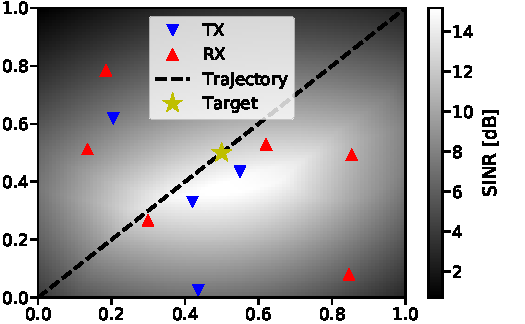
\includegraphics[width=.6\textwidth]{figures/MAB/env.pdf}
    \caption{Simulation setup.
    The target position is shown for the stationary case and the trajectory for the non-stationary case. 
    The heat map indicates the mean channel SINR at every position when the target scattering coefficient is excluded and all the channels are active.}
    \label{fig:env}
\end{figure}

\subsubsection{Reward distribution}

The agent aims to find the super arm which has the highest reward based on the equation \eqref{eq:reward_func}. 
To create the arm rewards, we define an instantaneous SINR measure $\esinr$ that satisfies $\E{\esinr} = \esinrexp$ where $\esinrexp$ is the channel SINR. 
The value $\esinr$ is calculated using the equation \eqref{eq:sinr} where the expectation is replaced with the power measurement $\esp$. 
To simplify the simulations, 
the target scattering coefficient $c$ remains constant through a single measurement period and the stochasticity of the noise and the interference powers in the measurements are approximated to be negligible. 
Therefore, the rewards for each arm are simulated by
\begin{equation}
    \esinr  \sim \text{Exp}\left(\esinrexp\right),
\end{equation}
which is the exponential distribution with mean of $\esinrexp$.
The channel SINR $\esinrexp$ on a linear scale for receiver $n$ and transmitter $m$ is calculated from the models defined in Sections \ref{sec:sys_conf}, \ref{sec:sc_model}, and \ref{sec:env_model} as follows
\begin{equation}
    \esinrexp = \frac{\epl \ercs \epower}{\thnoise + \eintnoise},
\end{equation}
where the transmit power $\epower=1$ is constant in time and equal for each transmitter.


\begin{figure}[!tb]\centering
    \subfloat[Stationary case.]
    {
        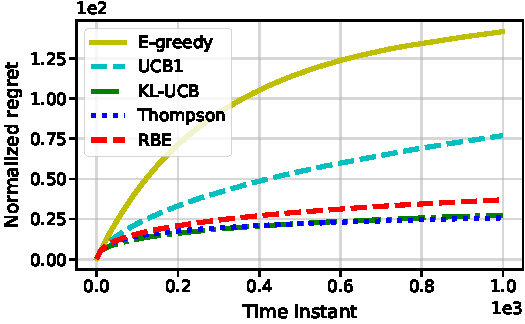
\includegraphics[width=.45\textwidth]{figures/MAB/stationary/cmab/regret.pdf}
        \label{fig:stationary_regret}
    }
    \hfill
    \subfloat[Non-stationary case.]
    {
        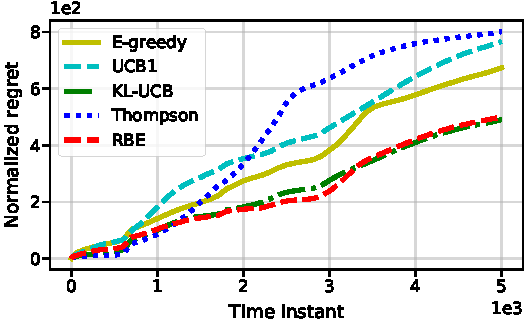
\includegraphics[width=.45\textwidth]{figures/MAB/non_stationary/regret.pdf}
        \label{fig:non_stationary_regret}
    }
    \caption{The normalized regret at each time instant. 
            RBE and KL-UCB perfom well in the both cases.}
    \label{fig:regret}
\end{figure}

\begin{figure}[!tb]\centering
    \subfloat[Stationary case.]
    {
        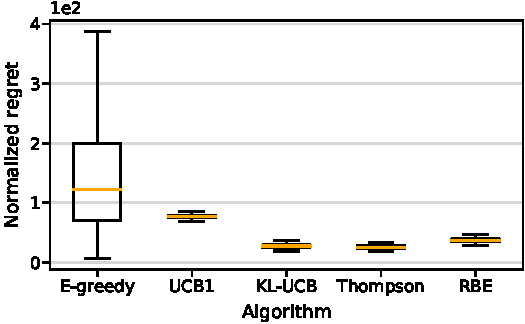
\includegraphics[width=.45\textwidth]{figures/MAB/stationary/cmab/regret_box.pdf}
        \label{fig:stationary_ci}
    }
    \hfill
    \subfloat[Non-stationary case.]
    {
        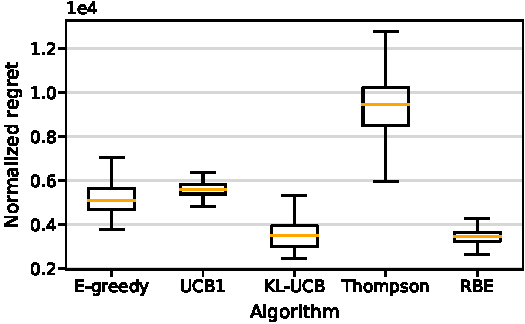
\includegraphics[width=.45\textwidth]{figures/MAB/non_stationary/regret_box.pdf}
        \label{fig:non_stationary_ci}
    }
    \caption{The normalized regret for the whole time horizon compared between different simulation runs.
            RBE and KL-UCB obtain excellent results in both stationary and non-stationary scenarios.}
    \label{fig:ci}
\end{figure}

\begin{figure}[!tb]
    \subfloat[Stationary case.]
    {
        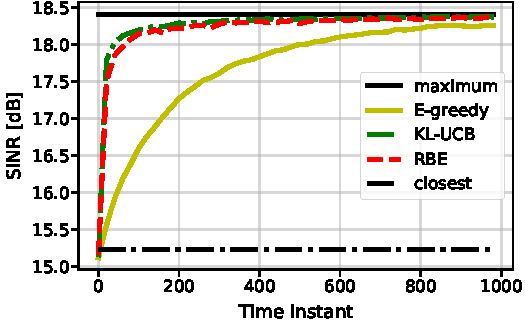
\includegraphics[width=.45\textwidth]{figures/MAB/stationary/cmab/sinr.pdf}
        \label{fig:stationary_sinr}
    }
    \hfill
    \subfloat[Non-stationary case.]
    {
        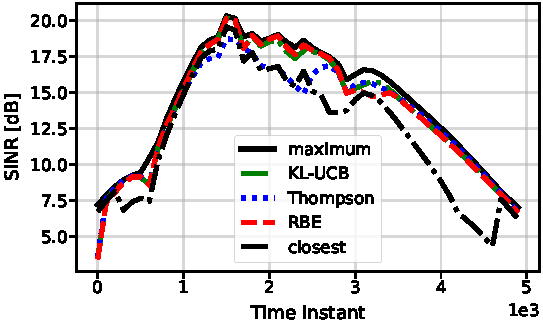
\includegraphics[width=.45\textwidth]{figures/MAB/non_stationary/sinr.pdf}
        \label{fig:non_stationary_sinr}
    }
    \caption{Reward at each time instant.
    The reward is a mean of the channel SINRs in a linear scale for the selected subset.
    The MAB algorithms are compared to a simple exploration-free method in which the subset of the receivers and the transmitters closest to the target is selected.
    In average, most of the MAB algorithms achieve a reward close to the maximum reward.}
    \label{fig:sinr}
\end{figure}

\subsection{Simulation results}

Two different scenarios are studied in the simulation examples. 
In the stationary scenario, there is a target that remains stationary at position $(0.5, 0.5)$.
In the non-stationary scenario, a target moves from $(0, 0)$ to $(1, 1)$ on a linear trajectory with a constant velocity.
All other parameters for the environment remain the same in both scenarios.
The five algorithms that were briefly reviewed in section~\ref{sec:MAB} are used in the simulations.
In addition, a simple method that selects the closest subset at each time instant is used to compare the MAB algorithms to a more conventional exploration-free method. 
The performance of the different MAB algorithms were evaluated using Monte Carlo simulations with $1000$ iterations.

The MAB algorithms are compared between each other in terms of regret. 
The regret through the simulation period is shown in Fig~\ref{fig:regret}. 
Also, box plots of the regrets are shown in Fig~\ref{fig:ci}.
The comparison between the exploration-free method and MAB algorithms is performed by comparing expectation of the achieved rewards through the simulation period.
The achieved rewards for two well-functioning MAB algorithms, 
the worst MAB algorithm and the exploration-free method are shown in Fig.~\ref{fig:sinr}.
The overall results show that the MAB algorithms improve the performance through the time horizon and outperform the exploration-free method in stationary and non-stationary cases.
Moreover, the RBE algorithm stands out with excellent reliability and regret performance in both cases.

\subsubsection{Stationary target}

In the stationary case, the discount factor can be set to $\alpha=t^{-1}$.
The value of $\epsilon$ for $\epsilon$-greedy exploration is set to 0.1, which means that it explores random subsets 10\% of the time.
Lower $\epsilon$ can sometimes result in lower regret, but the variance of the regret may increase.
The value 0.1 was found empirically in this simulation.
The other algorithms do not have any tunable parameters.
The time horizon is set to 1000 which is sufficiently long for finding the optimal TX-RX configuration.

The stationary target implies that the expected rewards of the arms do not change in time.
Therefore, it is possible to achieve a logarithmic regret \cite{Lattimore2019}.
From Fig.\ref{fig:stationary_regret} it can be observed that all algorithms other than $\epsilon$-greedy can achieve the sublinear regret.
Algorithms like Thompson sampling and KL-UCB which require knowledge about the reward distribution have excellent performance in these simulations.
The $\epsilon$-greedy algorithm has the highest regret and it is visible from Fig.\ref{fig:stationary_ci} that such random policies have a high variance.
Algorithms with higher variance make the learning less reliable even though they can some times find the optimal action faster than more reliable algorithms.

Fig.$\ref{fig:stationary_sinr}$ visualizes the achievable reward at each time instant.
The main difference between the MAB algorithms is the time taken to find the optimal super arm.
The gap between the maximum achievable reward and achieved expected reward will decrease as a function of time for algorithms that achieve sublinear regret.
Therefore, $\epsilon$-greedy with constant exploration probability will eventually have a constant gap between maximum reward and achievable expected reward.
It can be observed that the MAB algorithms perform much better than the exploration-free method.

\subsubsection{Non-stationary target}


The algorithms adapt to the non-stationary conditions by using the discounted action-value and discounted exploration parameters.
The discount factor is set to $\alpha = 0.998$.
Also, each element of $\vsinrb$ is divided by the maximum value before calculating the index.
This ensures that enough exploration is done at each time instant even if the scale of the rewards changes over time.
The value of $\epsilon$ for $\epsilon$-greedy algorithm is kept at 0.1.
The asymptotic optimality cannot be achieved since the exploration bonus will never vanish completely.
However, the considered algorithms have differences in their exploration efficiencies, as can be observed from the different regrets in Fig.\ref{fig:non_stationary_regret}.

In Fig.~\ref{fig:non_stationary_regret} it can be seen that KL-UCB and RBE achieve the lowest regret in the non-stationary case.
Thompson sampling does not adapt as well for the non-stationary case even if it performed quite well in the stationary case.
The $\epsilon$-greedy algorithm has lower regret than Thompson sampling but it still performs worse than the other algorithms. 
The Fig.\ref{fig:non_stationary_ci} demonstrates that RBE algorithm has a very small regret with low variance.
Also, the median performance is better than with any other of the used algorithms.
Hence it is promising algorithm for the radar problem at hand. 
The other algorithms which performed well in stationary reward scenario have poorer performance in non-stationary reward case.
The changes in reward distributions will force the agent to switch the arm if the action-value for the arm under exploitation becomes lower than the other action-values.
Therefore, in case of non-stationary target, the $\epsilon$-greedy algorithm achieves a smaller variance on regret than with stationary targets.

The achieved rewards are compared in Fig.\ref{fig:non_stationary_sinr}.
All MAB algorithms perform on average better than the exploration-free method through the whole simulation period.
Also, it is visible that the MAB algorithms can reach a SINR value close to the maximum reward at most of the time instances. 
Moreover, the performance gap between MAB algorithms is not as significant as in the stationary scenario.

\subsection{Summary}
\label{sec:tx_rx_summary}
The transmitter-receiver subset selection problem, in which the channel SINR values are unknown, was considered for the distributed MIMO radars.
Since only a subset of the channels can be selected at the same time, it was shown that such problems have to deal with the exploration-exploitation trade-off to identify the optimal subset without degrading the radar performance.
The problem was formulated as the combinatorial multi-arm bandit problem and reinforcement learning algorithm was proposed to solve the problem.
It was shown that reinforcement learning can be effectively used to continuously improve the subset selections and outperform the proposed exploration-free method.



\newpage
\section{Reinforcement Learning approach for Revisit Interval Selection}\label{sec:rl_ri}

In this Chapter, Reinforcement Learning (RL) methods are used to approach the Time Budget Management (TBM) problem described in Chapter \ref{sec:existing_RRM}.
An optimal Stochastic Dynamic Programming (SDP) technique for the TBM problem is unfeasible. 
Moreover, applying RL techniques to approximately find an optimal solution without using any relaxations can be challenging because of two reasons
\begin{enumerate}
    \item number of targets can change in time, and
    \item the TBM problem is Partially Observable Markov Decision Process (POMDP)
\end{enumerate}
The first difficulty affects the dimensions of the state and action spaces. 
For example, in multitarget tracking, the observation could be a combination of belief states of each target, and the action could be to choose which tracks will be updated next.
In that case, the number of actions would depend on the number of targets, and if an observation is presented as a matrix, the dimension of the matrix would depend on the number of targets.
Obviously, discretizing the observation space would not help either, since the number of discrete observations would grow exponentially as the number of targets increased.

The second difficulty is related to a more general problem with sensing systems,
the variables derived from the radar measurements always include a certain degree of uncertainty.
However, there are at least a couple of different ways to tackle the POMDP problems using reinforcement learning.
For example, a Markov Decision Process (MDP) state can be approximated from the sequence of past observations with finite length, or an external model-based approach can be used to extract the belief state.
The former approach can be implemented by stacking observations to form a single state as in \cite{Mnih2013}, or by using recurrent neural networks as in \cite{Hausknecht2015}.
The downside is that typically such approaches require a large amount of training.
In the latter approach, the RL policy is dependent on the model, thus modeling errors can decrease the performance of the policy.
However, in radar applications, the latter method is still attractive since typically required models already exist and training can faster compared to the former approach.

To avoid the difficulty with the variable number of targets, an optimal TBM problem is relaxed to an easier problem using the same techniques that were discussed in Section \ref{sec:RRM_tech}.
Especially, the TBM problem is addressed with a rule-based approach, in which adaptive Revisit Interval Selection (RIS) algorithms can be used to select the Revisit Interval (RI) of the tracking filter.
This approach enables using the RL policy for each track separately, thus making the actions and observations easier to present.

The proposed RL formulation is assuming a single target tracking (STT) scenario. 
Therefore, the formulation is not addressing the track association and implementation of the low-level scheduler.
However, the RL approach is extendable to multi-target tracking (MTT) scenarios by using a low-level scheduler and by considering the probability of mixing tracks with providing relevant observations for the RL agent.
In STT scenario, it is possible to experiment if the learning-based approach can help to tackle problems caused by modelling inconveniences that affect conventional non-learning-based algorithms.
The performance of the RL approach is investigated in benchmark trajectories proposed in \cite{Blair1998} by evaluating the probability of losing a track (PLT) and tracking load.

In the next sections, an RL approach is proposed for the RIS problem and evaluated using Monte Carlo simulations.
Section \ref{sec:system_description} describes the considered radar systems.
In Section \ref{sec:RL_formulation}, the RL formulation of the RIS problem is proposed for the radar system introduced in Section \ref{sec:system_description}.
In Section \ref{sec:ri_sim} the proposed RL approach is evaluated using the benchmark trajectories and a baseline algorithm.


\subsection{Assumed radar system} \label{sec:system_description}

The actions, observations, and rewards of the RL formulation are dependent on the radar system in which the RL algorithm is applied.
In other words, the system prescribes the available information to use as rewards and states, and the possible actions of the radar system.

The assumed radar system searches new targets using the search function. 
A track is initiated for a target before entering the tracking loop. 
In the assumed radar system, the tracking loop is implemented by the following steps.
\begin{enumerate}
\item\textbf{Predict the target position at the current time instant denoted as $t_k$.}

The target position is predicted using a tracking filter. The prediction is implemented by propagating the predictive tracking equations with an arbitrary processing interval $\dt$. The RI is selected such that the following equation holds $ \ri  =L \dt$ where L is an integer.

\item\textbf{Illuminate target at the predicted position.}

The center of the beamlobe is directed to the predicted target position. 
The center beam SNR is assumed to be a constant variable $SN_0$ if the predicted angle is exactly the target angle. 
On the other hand, if angle error exists, the SNR will degrade depending on the radar beamshape. 
In real-world radar, the center beam SNR could be kept approximately constant by adaptively controlling the transmit power using for example the Equation \eqref{eq:radar_snr} and the estimated target range. 
Another way to control the SNR is to use different integration times which affects the dwell time. 
It would add another dimension to the TBM problem. 
However, the only constant integration time is assumed here.

\item\textbf{If detection occurs, correct the target state estimate with the obtained measurement. If no detection obtained, either return to step 1 if the number missed detections is below a threshold $n_{max}$, or otherwise flag the target lost and exit the track update loop.}

In the latter case, the target is considered lost and it is not required to address here how the radar responds to such a scenario. 
In some radars, the track could be kept in memory if the target is found again for example by the search function. 
Then, the tracking loop could be restarted.


\item\textbf{Select the RI $\ri$.}

The RI is selected by using a RIS algorithm.
For example, using RIS algorithms reviewed in Section \ref{sec:tbm_ri} or the RI could be selected by an RL agent.

\item\textbf{Return to step 1 before time instant $t_k + \ri$.}

The certainty in the predicted state estimates will degrade in the function of time. Therefore, $t_k + \ri$ is the deadline for updating the track, but it could be also updated before the deadline depending on the higher-level implementation of the RRM.

\end{enumerate}

The track loop would be the same for each target in the MTT scenario. 
However, in the assumed STT tracking scenario only one tracking loop can occur. 
The STT scenario also simplifies the problem such that track association is not needed to consider.


\subsection{Reinforcement learning formulation}\label{sec:RL_formulation}

The RL formulation is proposed for algorithms such as Q-learning \cite{Sutton2018}, which have discrete action and state spaces. 
Therefore, the cardinality of the action and state spaces must be tolerable because otherwise, the exploration would take too much time.
In Section \ref{sec:actions} two different ways to present the action space are introduced.
Section \ref{sec:rewards} proposes a reward function that prevents losing tracks based on a certain cost and minimizes the tracking load. 
Finally, in Section \ref{sec:states} discrete observations are identified which at least approximately present valid MDP states in the RIS problem.

\subsubsection{Actions} \label{sec:actions}

\newcommand{\amax}{a_\text{max}}
\newcommand{\amin}{a_\text{min}}

The RL agent can control the RI using two different approaches.
One approach is to select the RI from a set of intervals.
This approach will be referred as direct selection.
The other approach either decreases or increases the RI with arbitrary delta value, that is referred as delta selection.
In other words, the action is mathematically interpreted as follows
\begin{equation}
    \ri(k) = \left\{
        \begin{array}{l l}
            A_k & \text{if direct selection used} \\
            \ri(k-1) + A_k &  \text{if delta selection used}
        \end{array}\right.
\end{equation}
where $A_k$ is the action taken at time instance $k$, and $\ri(k)$ is the RI selected at time instance $k$.
Both of the approaches could have either a continuous or a discrete action space.
In fact, the discrete action space is just a discretized version of the continuous action space $A_k \in [\amin, \amax]$.

The action space for direct selections is discretized such that subsequent RIs have equal distance.
In addition, maximum RI $\tmax$ and minimum RI $\tmin$ are loosely defined by using expert knowledge of by using trial and error approach in the simulations. 
By loosely defining it is meant that $\tmin$ can be shorter RI than the radar will ever use and similarly $\tmax$ can be longer.
An example set of actions for direct selections is $A_k \in \{0.5, 1.0, 1.5, 2.0, 2.5\}$, where $\tmax=2.5$, $\tmin=0.5$ and size of the action space is $5$.
In general form, the action space for direct selections is defined as follows
\begin{equation}\label{eq:as_direct}
    \Asdir \coloneqq \{ \frac{n \tmax + (\nacts-n-1) \tmin}{\nacts-1} \}_{n=0}^{\nacts-1},    
\end{equation}
where $\nacts$ is the size of the action space.
Lower $\nacts$ enables faster learning since there are less actions to be explored.
However, larger $\nacts$ may enable higher performance since larger variety of RIs could be used.

The action space for delta selections is defined using equal number of decreasing and increasing delta values. 
In addition, the action $a=0$ is included that neither increases or decreases the RI.
The deltas are are spaced with uniform distance as in \eqref{eq:as_direct}.
The maximum action $\amax=\deltalim$ and minimum action $\amin=-\deltalim$ are defined using the parameter $\deltalim$ which should be chosen along with the parameter $\nacts$ to achieve sufficiently large deltas with satisfactory resolution.
An action space for delta selection could be for example $\{ -1.0, -0.5, 0, 0.5, 1.0 \}$, where $\deltalim=1$ and $L=5$.
The general form of delta selection action space is
\begin{equation}\label{eq:as_delta}
    \Asdelta \coloneqq \{ \frac{\deltalim \left( 2 n - \nacts + 1 \right)}{\nacts-1} \}_{n=0}^{\nacts-1},
\end{equation}
where $\nacts$ should be positive odd number.
It is not required to define the limits $\tmax$ and $\tmin$ unlike in the direct selection. 
In addition, $\deltalim$ can be much lower than $\tmax - \tmin$.
However, multiple actions might be needed to achieve the desired RI which depends on $\deltalim$ and $\nacts$.

\subsubsection{Reward} \label{sec:rewards}

\newcommand{\ploss}{P_\text{loss}}

\newcommand{\pref}{P_\text{ref}}
\newcommand{\lref}{L_\text{ref}}

The overall objective for the agent is to minimize time budget needed to maintain a track, and prevent track losses based on a cost of a track loss.
The objective should be reflected in the immediate and cumulative rewards that are given for the RL agent as in Equation \ref{eq:discounted_sum}. 
However, it is not compulsory to account the long-term rewards if it is not required for the RL formulation.
The proposed immediate rewards are
\begin{equation}
    r = \left\{
    \begin{array}{ll}
        -\frac{n}{\ri} \tau, & \text{in case of detection,}\\
        -\closs, & \text{otherwise}.
    \end{array} \right.
\end{equation}
where $\tau$ is dwell length and $n$ is number of dwells needed to achieve a detection, and $\closs$ is cost for losing a track.
The immediate reward emphasizes target to minimize tracking load by using tracking load as a penalty.
In addition, the cost $\closs$ is used to prevent agent from losing a track while minimizing the load.
The discount factor $\lambda$ can be used to control if future tracking load and possibility to lose track is also accounted.
The agent is capable of trading immediate performance for better long-term performance when $\lambda > 0$.
However, in myopic case when $\lambda = 0$, RL algorithms will converge faster.

The value for $\closs$ is found by using a heuristic design rule, which is based on simplified two state MDP.
The states of the MDP represent if target is lost or not.
An agent needs to select an action from two competing actions.
One of the actions, denoted as $a_1$, will have tracking load of $\lref$ and the PLT is zero.
For the other action, the PLT is one, and the action is denoted as $a_2$.
The parameter $\closs$ should be defined such that
\begin{equation}\label{eq:closs_criterion}
    \sum_{i=0}^\infty \lambda^i \lref = \closs
\end{equation}
which indicates that the discounted sum of rewards when taking action $a_1$ should be equal to the penalty of losing track if action $a_2$ is taken.
Equation \eqref{eq:closs_criterion} can be rewritten into form
\begin{equation}
    \closs = \frac{1}{1-\lambda} \lref
\end{equation}
 by using geometric series.

To understand the rewards in more detail, an expected value is examined.
The expected value of a immediate reward given the state $s$ and action $a$ is
\begin{equation}\label{eq:exp_reward}
    \E{R_{t+1} | S_t=s, A_t=a} = -(1-\ploss(s, \ri)) 
        \frac
        {
            \mathbb{E} \left[ n | s, \ri \right]
        }
        {
        \ri
        } 
        - \ploss(s, \ri) \closs
\end{equation}
where $\ploss(s, \ri)$ is the PLT given the state $s$ and RI $\ri$, and $\E{n|s, \ri}$ is expected value of the number of dwells.
Equation \eqref{eq:exp_reward} is also the action-value in myopic case.
The expected value of a non-myopic action-value is a little bit more complicated to write since the MDP can end if the track is lost.
Therefore, 
\begin{align}
    \E{\sum_{i=0}^\infty \lambda^i R_{t+1} | S_t=s, A_t=a} =& \E{R_{t+1} | S_t=s, A_t=a} + (1-\ploss(s, \ri)) \lambda \\
    & \sum_{s'\in \Ss} p(S_{k+1}=s'|S_{k}=s, A_{k}=a)  V(s')  
\end{align}
where $(1-\ploss(s, \ri))$ shows that the non-myopic part is weighted by the probability of not losing the track.

\subsubsection{States and observations} \label{sec:states}

\newcommand{\glow}{g_\text{low}}
\newcommand{\ghigh}{g_\text{high}}

The observations given for the agent are critical since those are the only of information for the agent to know in which situation it is operating currently.
In RL, an observation is generally a partial observation from an environment state.
The environment state describes all the information that is needed to determine how the environment responds to an action of the agent. 
An observation or sequence of observations is denoted as agent state.
The agent state contains the information that is available and relevant for the agent to choose an action.
Moreover, the achievable quality of the actions can be dependent on the amount of information that is available. 

For Q-learning algorithm, the agent state needs to be discrete and approximately Markovian.
The information from the radar system is typically provided by continuous variables and therefore discretization is required.
The continuous variables are discretized as follows. 
Two states are defined for values below $\ghigh$ and above $\glow$. 
The remaining states are defined by using the following equation 
\begin{equation}\label{eq:state_limits}
    \frac{\ghigh - \glow}{N_d - 2} n + \glow
\end{equation}
where $N_d$ is number of discrete states and $n \in \{0, 1, ..., N_d-1\}$ is the index of the discrete state.
For $n$th state, lower limit is obtained by calculating equation \eqref{eq:state_limits} with $n$ and upper limit with $n+1$.
Discretizing multiple variables will lead to exponentially growing cardinality.
In some cases, the requirement for approximately Markovian state can be fulfilled by using a subset of past actions and observations \cite{Mnih2013}, but for discrete states the cardinality of the state space will grow exponentially.


In RIS problem, 
the environment state includes for example the target kinematic state and corresponding belief state obtained by the tracker. 
The belief state and any signals from the radar can be used as an agent state, but only significant information need to be extracted for more efficient learning. 
One good source of information from the tracking filters is innovation sequence. 
It includes information about how well the tracker did predict the target position compared to the position estimate derived from a temporal radar measurement. 
In addition, 
the radars utilizing the Doppler phenomena, 
range-rate can be examined. 
The simplest way to utilize innovation sequence in discrete RL algorithms, is to use the last innovation as a state. 
The size of the state space can be further reduced by using only the innovation in angle since it assumed that the target range is less important for steering the radar beam into correct direction. 
The state is not fully Markovian since the temporal angle estimates may contain noise. 

Another appealing option is to use the mode probabilities $\mu$ as a state if the tracking filter is multiple model estimator such as Interactive Multiple Model (IMM) estimator. 
The number of discrete states remain tolerable as long as the number of discrete probabilities and modes are sufficient to prevent the exponential growth of the cardinality. 
An similar approach in which the mode probabilities are used was presented in equation \eqref{eq:fimm} which calculates the RI using the mode probabilities and the steady-state RIs. 

The state presentations based on the innovation or on the mode probabilities can be further extended by augmenting previous RI to the state.
Also, two additional states are included to the state space. 
One for lost target and other for track initiation.
The latter state enables agent to learn RIs at the beginning of the tracking task where tracking filter might have unreliable estimates.
The number of discrete states is $N_s = 2+N_d$ if the previous RI is not included into state and $N_s = N_d N_a + 2$ otherwise.
In Section \ref{sec:training}, the most effective state presentation will be identified among the different state spaces presented here.


\begin{figure}[t]
    \centering
    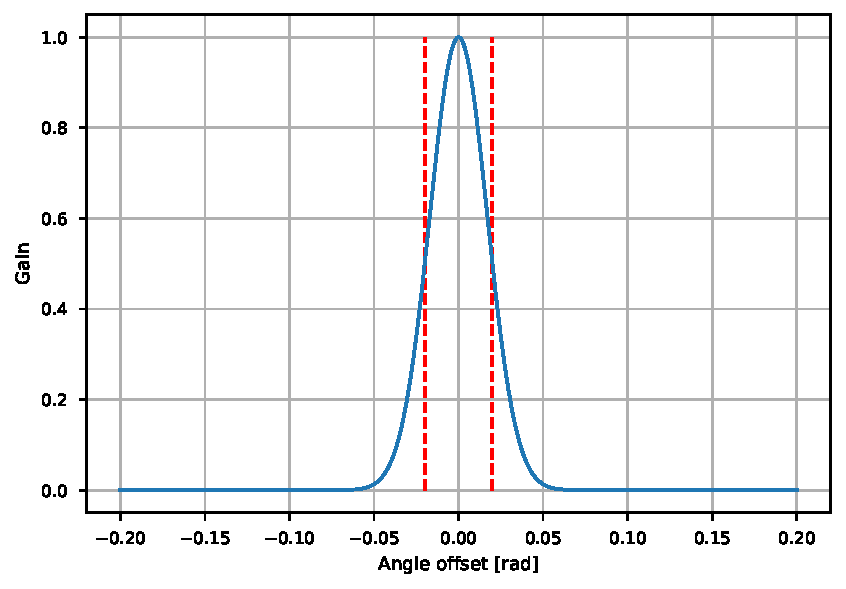
\includegraphics[width=0.68\textwidth]{figures/benchmark/beamwidth.pdf}
    \caption{Receive gain in linear scale in function of the beam offset. 
    The half-power offset angles are illustrated with red lines.}
    \label{fig:beamwidth}
\end{figure}

\subsection{Simulation setup}\label{sec:ri_setup}

\newcommand{\sno}{SN_0}



\bgroup
\def \arraystretch{1.25}
\begin{table}[tb]
    \centering
    \begin{tabular}{|l|c|c|c|}
    \hline
    \textbf{Name}              & \textbf{Symbol} & \textbf{Value}  & \textbf{Unit}\\ \hline
    Boresight SNR              & $SN_0$          & $50$ & -          \\ \hline
    Range resolution            & $r_\text{res}$  & $10$ & m  \\ \hline
    Monopulse antenna pattern slope  & $k_m$      & $1.6$ & -  \\ \hline
    Half of the $-3$dB beamwidth & $B$             & $0.02$ & rad         \\ \hline
    Probability of false alarm & $P_\text{fa}$   & $10^{-6}$ & -      \\ \hline
    Maximum number of dwells   & $n_\text{max}$  & $20$ & -  \\ \hline
    Dwell time                 & $\tau$          & $1e-3$ & s   \\ \hline
    Position                   & -               & $(0, 0)$ & m \\ \hline
    \end{tabular}
    \caption{Radar parameters in the simulations. Note that the probability of false alarm is only used to calculate the probability of detection.}
    \label{tab:radar_parameters}
\end{table}
\egroup

The RL approaches are evaluated using target trajectories from a benchmark problem proposed in \cite{Blair1998}. 
Subsection \ref{sec:benchmark_trajectories} introduces the benchmark trajectories in more detail. 
The simulation scenario contains the assumed monostatic radar presented in Subsection \ref{sec:system_description} at the position $x=0$ and $y=0$. 
The probability of detection is simulated based on Swerling I RCS model as follows
\begin{equation}\label{eq:singer_1_pd}
    P_\text{d} = P_\text{fa}^{\frac{1}{1+SNR}},
\end{equation}
where $P_\text{fa}$ is the probability of false alarm.
However, $P_\text{fa}$ is only utilized to calculate the probability of detection, and false alarms are not included into the simulations.
The target is considered lost after $\nmax=20$ dwells without a detection.
The angle offset of the radar beam is assumed to affect the SNR based on the following equation
\begin{equation} \label{eq:offset_snr}
    SNR = \sno~\exp{ - \ln{2}
        \frac
            {(\hat{\theta} - \theta)^2}
            {B^2}}    
\end{equation}
where $\sno=50$ is boresight SNR in a linear scale, $B=0.02$ is half of the -3dB beamwidth in radians, $\theta$ is target angle and $\hat{\theta} $ is the boresight angle. 
Furthermore, the parameters $\sno$ and $B$ are constant in the simulations. 
The radar beam is visualized in Figure \ref{fig:beamwidth}.
The fixed parameters of the simulated radar are summarized in Table \ref{tab:radar_parameters}.

The measurement model described in Subsection \ref{sec:measurement_model} is used to map the states to the measurements in the tracking filter.
In addition, the radar system is using an IMM estimator in which the Constant Velocity (CV) and the Constant Acceleration (CA) models presented in the Subsection \ref{sec:target_models} are used.
The configuration of the IMM estimator will be covered in more detail in Subsection \ref{sec:IMM}.


\subsubsection{Benchmark trajectories} \label{sec:benchmark_trajectories}

The target trajectories used in the simulations are based on a benchmark problem that was initially introduced in \cite{Blair1998}.
The original benchmark problem considered MTT in presence of electronic counter measure (ECM).
However, in the simulations the trajectories are used for STT scenario and false alarms are neglected.
For the sake of simplicity, the spatial dimension is downsized from 3D space to 2D space.
The 2D benchmark trajectory is shown in Figure \ref{fig:benchmark_trajectories}.
\begin{figure}[tb]
    \centering
    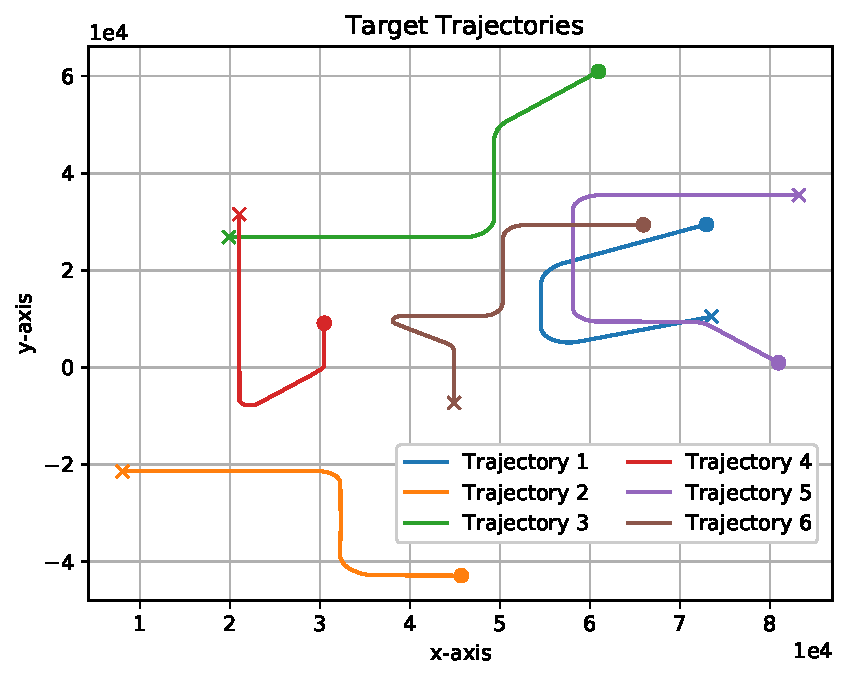
\includegraphics[width=0.7\textwidth]{figures/benchmark/trajectories.pdf}
    \caption{Six different target trajectories. The trajectory starts from "x" and ends to "o".}
    \label{fig:benchmark_trajectories}
\end{figure}
The trajectories include different kind of motion such as constant-g turns, turns with acceleration, and straight motion with constant velocity and  acceleration.
The target speed can range approximately from 210 m/s to 460 m/s as it can be seen from Figure \ref{fig:benchmark_velocities}.
The acceleration ranges approximately from 0 m/s$^2$ to 115 m/s$^2$ as it can be seen from Figure \ref{fig:benchmark_acceleration}.
The benchmark trajectories are further summarized in Table \ref{tab:benchmark_table} which contains mean and standard deviation values for acceleration and velocity in each trajectory.
The values are later in Subsection \ref{sec:IMM} utilized to select the IMM estimator parameters. 

\begin{figure}[htb]
    \centering
    \begin{subfigure}{0.45\textwidth}
        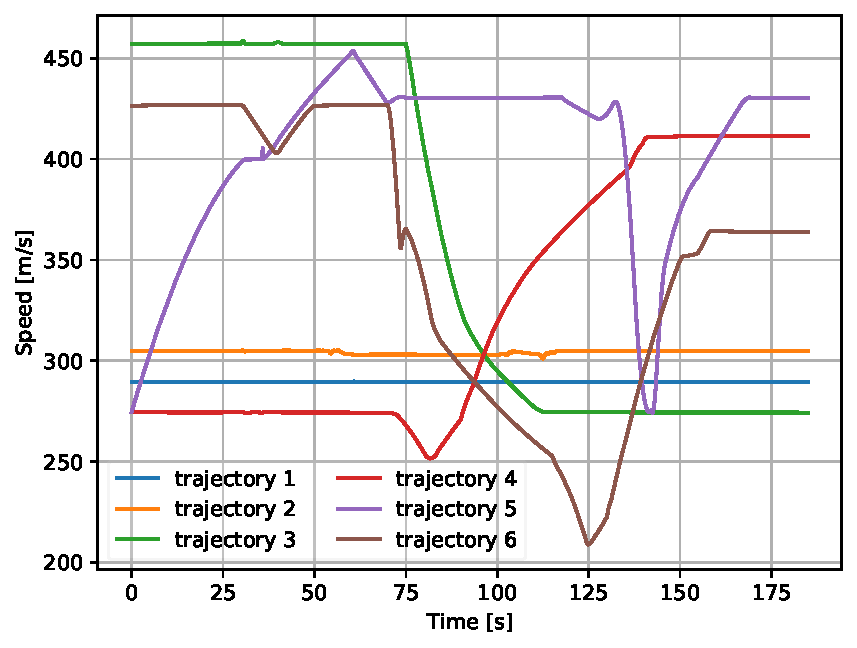
\includegraphics[width=\linewidth]{figures/benchmark/velocities.pdf}
        \caption{Target speed in function of time.}
        \label{fig:benchmark_velocities}
    \end{subfigure}
    \hfill
    \begin{subfigure}{0.45\textwidth}
        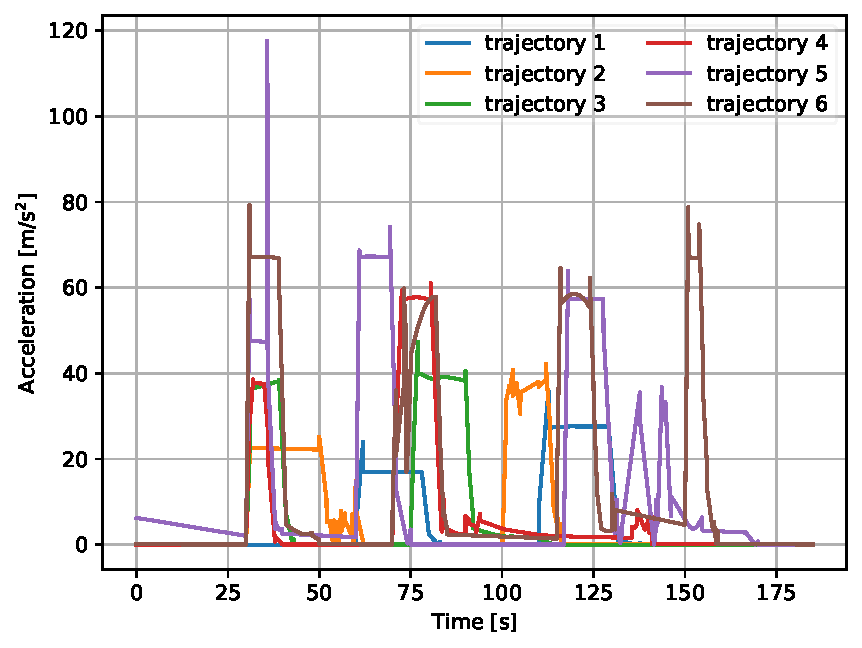
\includegraphics[width=\linewidth]{figures/benchmark/accelerations.pdf}
        \caption{Target acceleration in function of time.}
        \label{fig:benchmark_acceleration}
    \end{subfigure}
    \label{fig:benchmark_vel_acc}
    \caption{Acceleration and velocity visualized in function of time for benchmark trajectories. }
\end{figure}

\begin{table}[htb]
    \centering
\begin{tabular}{|l|l|l|l|l|l|l|l|}
\hline
\multicolumn{2}{|l|}{}                                 & \textbf{T1} & \textbf{T2} & \textbf{T3} & \textbf{T4} & \textbf{T5} & \textbf{T6} \\ \hline
\multirow{2}{*}{\textbf{Velocity}}     & \textbf{mean} & 160.47      & 116.54      & 184.89      & 304.76      & 189.37      & 199.29      \\ \cline{2-8} 
                                       & \textbf{std}  & 78.92       & 139.4       & 198.54      & 90.8        & 181.85      & 170.52      \\ \hline
\multirow{2}{*}{\textbf{Acceleration}} & \textbf{mean} & 4.72        & 5.38        & 5.44        & 5.51        & 11.87       & 12.83       \\ \cline{2-8} 
                                       & \textbf{std}  & 9.23        & 10.87       & 12.65       & 13.79       & 20.06       & 22.06       \\ \hline
\end{tabular}
    \caption{Benchmark trajectories summarized with mean and standard deviation values. Labels T1-T6 denote trajectories from 1 to 6. Unit for velocity values is in m/s, and m/s$^2$ for acceleration values.}
    \label{tab:benchmark_table}
\end{table}


\subsubsection{CVCA-IMM estimator}\label{sec:cvca_imm}

\newcommand{\varcv}{\sigma_\text{cv}^2}
\newcommand{\varca}{\sigma_\text{ca}^2}
\newcommand{\msp}{\mu}

The employed IMM estimator is using two linear Kalman filters configured for two target motion models, that are the CV and CA models described in Subsection \ref{sec:target_models}.
In addition, the measurement model described in Subsection \ref{sec:measurement_model} is used in both filters.
The configuration is simple, but the estimator can adapt to the various different maneuvers in the benchmark trajectories.
The mode transition probability from CV to CA and CA to CV is set to be equal such that the state transition matrix is
\begin{equation}
    M = 
\begin{bmatrix}
1 - \msp & \msp\\ 
\msp & 1 - \msp
\end{bmatrix},
\end{equation}
where $\msp$ is the mode transition probability.
The IMM estimator configuration will be referred as CVCA-IMM estimator.

There are couple reasons for using such a configuration.
First, the measurement and motion models are linear that is required for linear Kalman filters introduced in Subsection \ref{sec:kalman_filter}.
However, RL approach would be applicable for non-linear filters without changing the RL formulation.
Second, only one model probability is sufficient to present the state since the IMM estimator has only two models.
Lastly, the CVCA-IMM estimator has only three parameters to be tuned.
The parameters are the acceleration noise variance for CV model $\varcv$, the acceleration noise variance for CA model $\varca$, and the mode transition probability $\msp$.

The mode transition probabilities are defined for the processing time step $\dt=0.1$, because the tracker is using the time step to predict the future states recursively.
In other words, $\msp$ is the probability that the motion mode switches after time step $\dt$.
Sojourn time is the time that is expected for the system to spend in a specific state.
The transition probability $\msp$ can be then calculated by the following equation
\begin{equation}
   \msp = \frac{\dt}{T_s},
\end{equation}
where $T_s$ is the sojourn time.
However, the sojourn time is typically tedious to estimate for a target especially when using non-optimal motion models.
As described in \cite{Simeonova2002}, higher transition probabilities lead to lower peak errors but the mean error can be higher.
The parameters $\msp=0.028$, $\varcv=747.5$ and $\varca=74.7$ are found empirically, by simulating the CVCA-IMM estimator with various different parameter combinations.
The selected $\msp$ corresponds to approximately $3.6s$ Sojourn time.

There is still a problem that needs to be considered when using the two target models.
The vector dimensions of the CV state \eqref{eq:x_mode1} and the CA state \eqref{eq:x_mode2} are different. 
Moreover, the mode mixing equations \eqref{eq:imm_mx_init_x} and \eqref{eq:imm_mx_init_P} along with the state covariance fusion equations \eqref{eq:imm_fusion_x} and \eqref{eq:imm_fusion_P} require the dimensions to be equal.
In \cite{Granstroem2015}, an enhanced approach for mixing states with different dimensions was proposed.
However, here a simple approach is employed, which was also discussed in \cite{Granstroem2015}.
The approach augments the state estimate and corresponding error covariance matrix of the CV model with zeros.
According to \cite{Granstroem2015}, it corresponds to situation in which the distributions of thew accelerations in $x$ and $y$ coordinates are approximated with Dirac delta function.

\begin{figure}[bt]
    \centering
    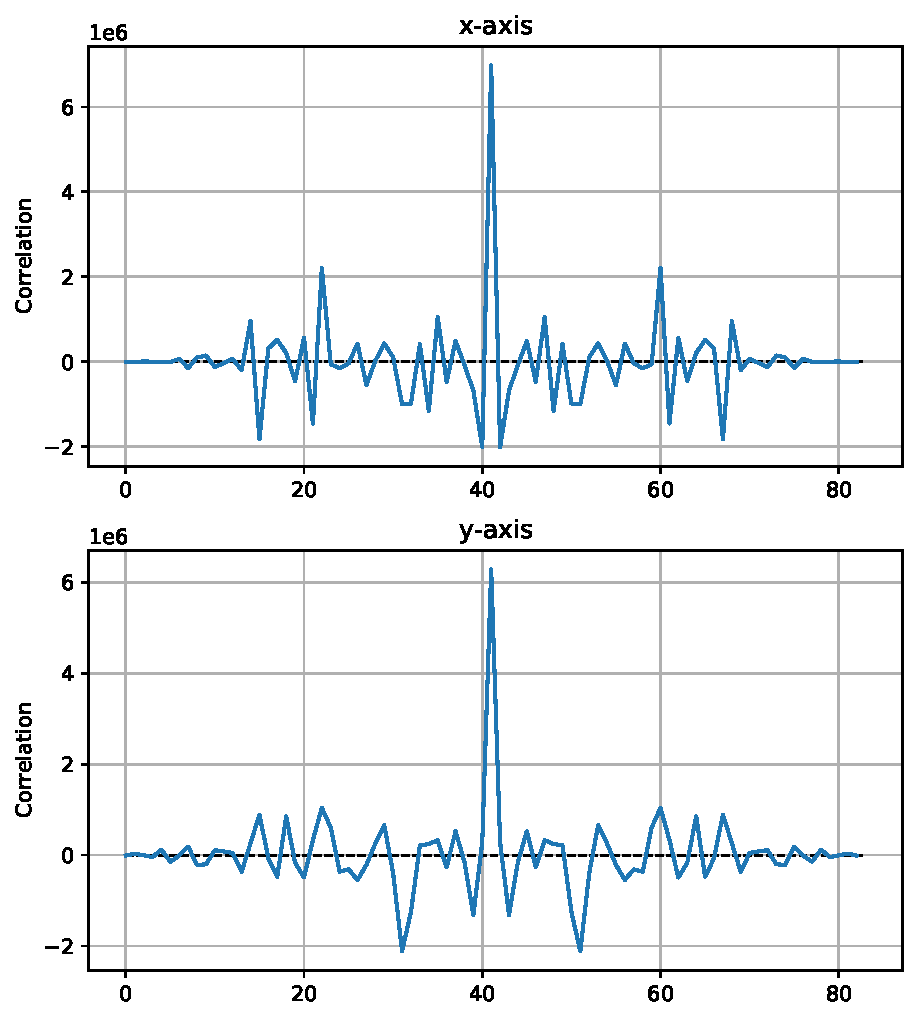
\includegraphics[width=0.7\linewidth]{figures/benchmark/IMM/correlation_imm.pdf}
    \caption{Auto-correlation of innovation sequence for the CVCA-IMM estimator.}
    \label{fig:auto_correlation}
\end{figure}

The performance of the tracking filter can be examined by visualizing the auto-correlation function of the innovation sequence.
In ideal case the auto-correlation function should not have large correlations which indicates that innovation sequence is approximately non-correlated noise.
Figure \ref{fig:auto_correlation} shows the auto-correlation function of the innovation sequence in $x$ and $y$ axis on trajectory 6.
From the figure, it can be seen that the auto-correlation function is mainly random such that he innovation sequence does not have significant correlations.
Thus, the CVCA-IMM estimator functions in the tracking scenario as desired.



\subsubsection{Baseline algorithm}

\begin{figure}[tb]
    \centering
    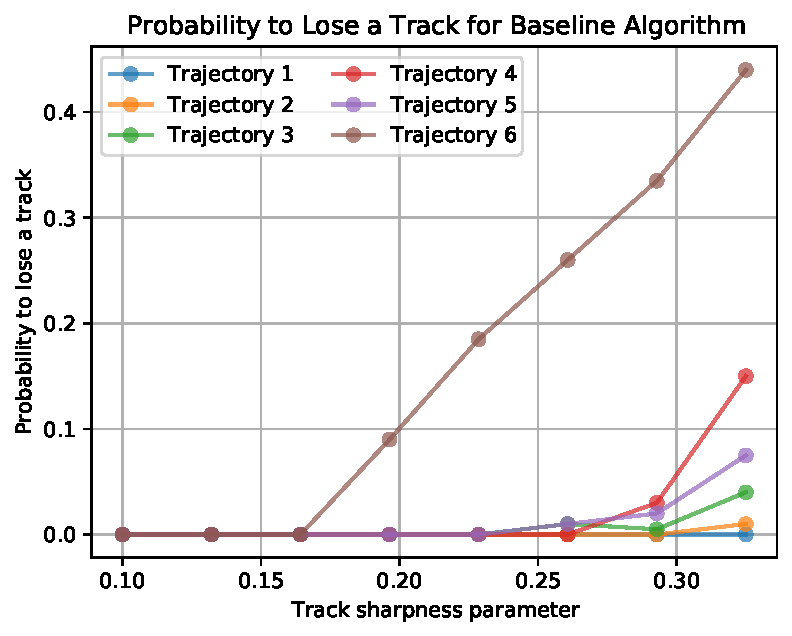
\includegraphics[width=0.7\linewidth]{figures/benchmark/Simulations/plt_baseline.pdf}
    \caption{Tuning track sharpness parameter $V_0$ for the baseline algorithm.}
    \label{fig:baseline_plt}
\end{figure}

A baseline algorithm is utilized for evaluating RL approach against existing RIS algorithm.
The baseline algorithm for controlling the RI is based on an approach proposed in \cite{Daeipour1994}.
The algorithm is error covariance matrix based algorithm, thus relies on the following inequality
\begin{equation}\label{eq:baseline_ineq}
    \sigma_\theta(t+\ri|t) \leq V_0 B, 
\end{equation}
where $V_0$ is the track sharpness parameter, and $\sigma_\theta(t+\ri|t)$ is error standard deviation on \prior estimate of the target azimuth angle $\theta$.
The highest RI to fulfil the Equation \eqref{eq:baseline_ineq} is found by propagating the predictive equations of the CVCA-IMM estimator with time step $\dt$.
The track sharpness $V_0$ affects PLT and needs to be tuned for the specific IMM estimator.
Different track sharpness values were evaluated for the benchmark trajectories by  using 200 Monte Carlo iterations per trajectory.
Figure \ref{fig:baseline_plt} shows the simulation results, and illustrates how $V_0$ affects the PLT. 


\subsection{Simulation results}\label{sec:ri_sim}

The RL approach will be evaluated in the simulation setup described in Section \ref{sec:ri_setup}.
The simulations are used
\begin{itemize}
    \item to identify effective state presentations,
    \item to determine is it sufficient to use myopic policy over non-myopic policy,
    \item to evaluate performance during learning,
    \item to evaluate the amount of learning needed achieve a certain level of performance,
    \item to determine connection between $\closs$ and PLT, and
    \item to compare RL approach against the baseline algorithm.
\end{itemize}
The first five of these will be covered in Subsection \ref{sec:training}, and the last one will be covered in Subsection \ref{sec:against_baseline}.

\subsubsection{Training RL agent}\label{sec:training}



Various RL agents are trained by uniformly sampling target trajectories from the six benchmark trajectories.
One training episode corresponds to simulating agent on a single trajectory as long as the end of the trajectory is reached or the target is lost.
Overall, each agent is trained for $4000$ episodes, which corresponds to training an agent on each trajectory approximately for $667$ times in expectation.

All the agents use Q-learning algorithm with \egreedy exploration.
The exploration probability is initially $\epsilon=0.2$ and between each episode the epsilon is decayed by a fraction of $0.99867$ which corresponds to $\epsilon=0.001$ on the last training episode.
The learning rate $\alpha$ is controlled adaptively by using the asynchronous update strategy \cite{Even-Dar2003}.
Thus, the learning rate is defined in function of time as follows
\begin{equation}
    \alpha_t = \frac{1}{\#(s, a, t)^\omega},
\end{equation}
where $\#(s, a, t)$ is the number of times action $a$ is taken from state $s$ at time instant $t$, and $\omega \in (0.5, 1)$ controls how fast $\alpha_t$ decays.
In myopic case, the parameter $\omega$ can be set $1$, when the empirical mean for action-values are calculated.

The action space with direct selections $\Asdir$ is used with $N_a=10,$ $\tmin=0.1s$ and $\tmax=7.5s$.
Furthermore, various agents are configured such that it is possible to identify effective state presentations from the states discussed in Section \ref{sec:states}, and to determine is it sufficient to use myopic policy over non-myopic policy.
The states presented in Section \ref{sec:states} are the innovation, the mode probability, and both can be augmented by the previous RI.
The discretization parameter is set to $N_d=10$, such that $N_s=12$ for state presentations without previous RI and $N_s=102$ otherwise.
For myopic agents the discount factor $\lambda=0$ and adaptive learning rate parameter $\omega=1.0$.
For non-myopic agents the corresponding values are set to $\lambda=0.7$ and $\omega=0.75$. 
The configurations of the agents are shown in Table \ref{tab:agent_configurations}, and the ID's from the table are used in the figures later.

\begin{table}[t]
    \centering
    \begin{tabular}{|c | c | c |c |}
        \hline
        \textbf{Agent id} & \textbf{State presentation}  & $\lambda$  &  $\omega$ \\
        \hline
        0 & innovation & 0.0 & 1.0 \\ \hline
        1 & innovation & 0.7 & 0.75 \\ \hline
        2 & innovation \& previous RI &  0.0 & 1.0 \\ \hline
        3 & innovation \& previous RI & 0.7 & 0.75 \\ \hline
        4 & mode probability &  0.0 & 1.0 \\ \hline
        5 & mode probability & 0.7 & 0.75 \\ \hline 
        6 & mode probability \& previous RI &  0.0 & 1.0 \\ \hline 
        7 & mode probability \& previous RI & 0.7 & 0.75 \\
        \hline
    \end{tabular}
    \caption{Agent configurations.}
    \label{tab:agent_configurations}
\end{table}

Target and behavior policies, discussed in Section \ref{sec:q_learning}, will be evaluated in function of number of training episodes.
The behavior policy includes the random actions of the epsilon greedy exploration strategy, and is used to evaluate the performance while learning.
On the other hand, the target policy takes the actions with highest action-values, thus is purely exploiting, and can be used to evaluate the amount of learning needed achieve a certain level of performance.
It corresponds to the situation where learning ends after certain number of episodes, and thereafter the agent uses only the target policy.
The performance of a behavior policy will be referred as offline performance, and similarly online performance for a target policy.

\begin{figure}[htb]
    \centering
    \begin{subfigure}[b]{0.7\textwidth}
        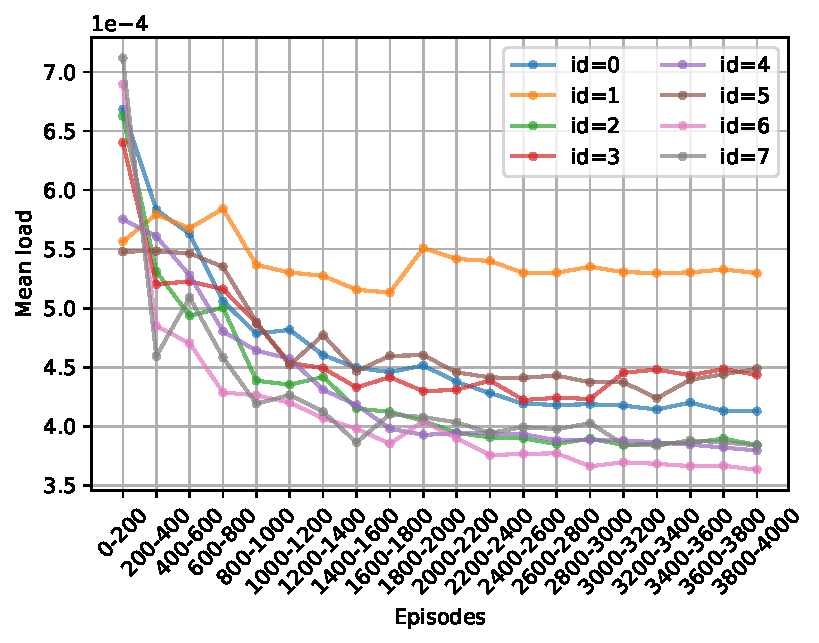
\includegraphics[width=\textwidth]{figures/benchmark/Training/online_load.pdf}
        \caption{Mean tracking load.}
        \label{fig:online_load}
    \end{subfigure}
    \hfill
    \begin{subfigure}[b]{0.7\textwidth}
        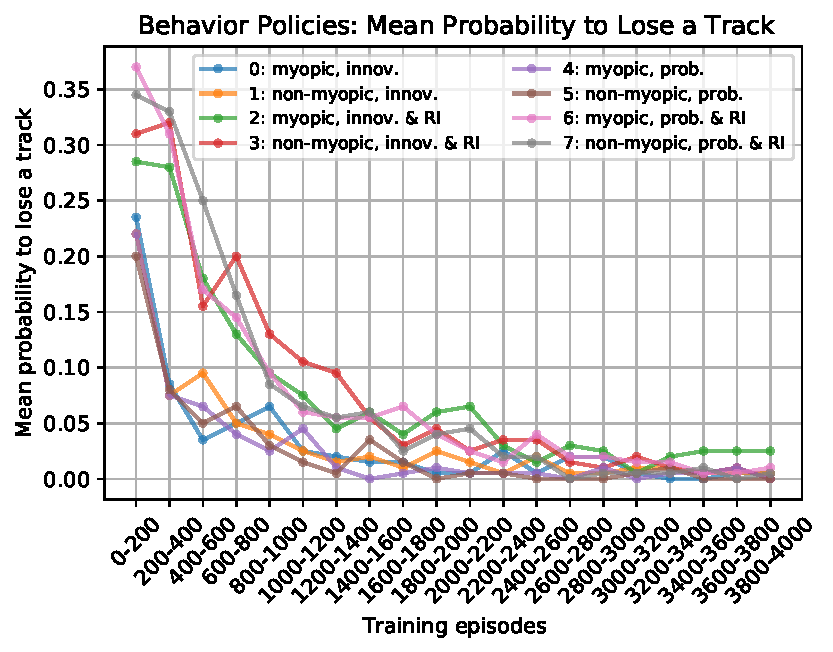
\includegraphics[width=\textwidth]{figures/benchmark/Training/online_plt.pdf}
        \caption{Probability to lose a track in an episode.}
        \label{fig:online_lost}
    \end{subfigure}
    \caption{Online performance estimated from the training data averaging over last 200 episodes.}
    \label{fig:online_performance}
\end{figure}

\begin{figure}[htb]
    \centering
    \begin{subfigure}[b]{0.7\textwidth}
        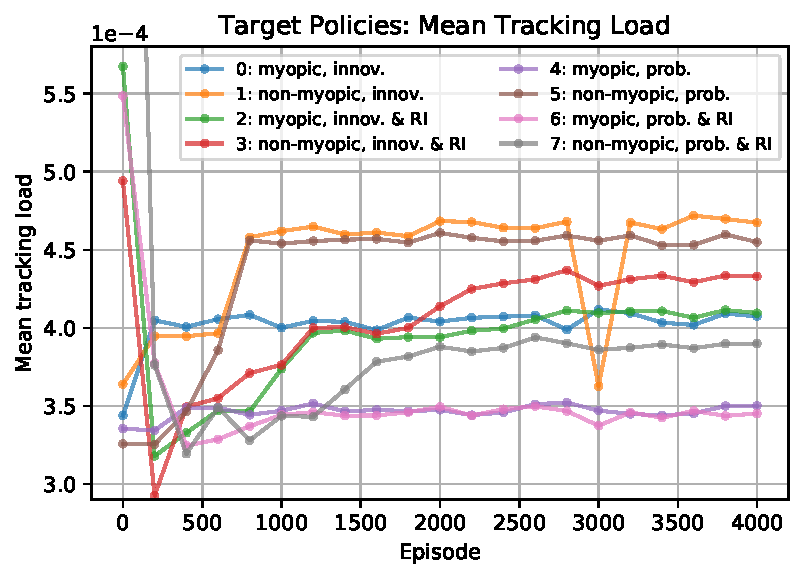
\includegraphics[width=\textwidth]{figures/benchmark/Training/offline_load.pdf}
        \caption{Mean tracking load.}
        \label{fig:offline_load}
    \end{subfigure}
    \hfill
    \begin{subfigure}[b]{0.7\textwidth}
        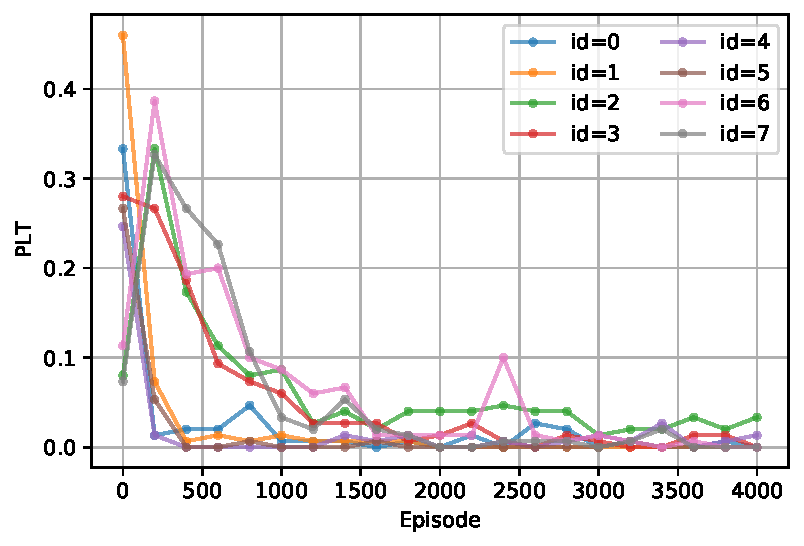
\includegraphics[width=\textwidth]{figures/benchmark/Training/offline_plt.pdf}
        \caption{Probability to lose a track in an episode.}
        \label{fig:offline_lost}
    \end{subfigure}
    \caption{
        Offline performance estimated from Monte Carlo simulations.
    }
    \label{fig:offline_performance}
\end{figure}

The offline and online performance are evaluated using criteria based on the tracking load in Equation \eqref{eq:load} and PLT.
The former criterion, denoted as mean tracking load, evaluates tracking load using the following equation
\begin{equation}\label{eq:criterion_load}
    L_\text{mean} = \frac{1}{M} \sum_{m=0}^{M-1} \frac{1}{K_m}\sum_{k=0}^{K_m-1} L_{mk}
\end{equation}
where $M$ is number of episodes, $K_m$ is number of steps in episode $m$, and $L_{mk}$ is the tracking load in episode $m$ at step $k$.
The latter criterion, denoted as mean PLT, is calculated as follows
\begin{equation}\label{eq:criterion_lost}
    \frac{1}{M} \sum_{n=0}^{M-1} \vec{1}_{\text{TrackLost}(m)}
\end{equation}
where $\vec{1}_{\text{TrackLost}(m)}$ is one if track is lost in episode $m$ and zero otherwise.

The behavior policies are evaluated every 200 episode while training and using the past M=200 training episodes to calculate \eqref{eq:criterion_load} and \eqref{eq:criterion_lost}.
The online performance evaluated with the aforementioned criteria are shown in Figure \ref{fig:online_performance}.
The target policies are also evaluated every 200 episodes. 
However, the snapshots of the target policies need to be separately evaluated using Monte Carlo simulations since training data can not be used.
Thus, each policy snapshot is evaluated with 25 Monte Carlo iterations per trajectory.
The offline performance is shown in Figure \ref{fig:offline_performance}.

From Figure \ref{fig:online_performance} it is apparent that the online performance is slowly improving between episodes with a certain trend.
On the other hand, the trend for offline performance is not as apparent as shown in Figure \ref{fig:offline_performance}.
Especially, the mean tracking load in Figure \ref{fig:offline_load} meets its lower limit quite fast, but the mean PLT in Figure \ref{fig:offline_load} will take more time to converge to tolerable levels.
The differences between online and offline performance may be explained by differences in target and behavior policies.
The behaviour policy takes the random actions that increase the tracking load compared to target policy which is purely exploiting.
For the agent, it is certainly much more challenging to learn the expected PLT than the tracking load when taking actions from different states.
Therefore, the offline tracking load converges to low values faster than the PLT.
Thus, learning to not lose tracks will take take more training episodes.
The offline mean tracking load rises a little bit when the agent has learnt more because the agent becomes more conscious about losing track with longer RIs.

In episodes approximately up to 1500, two distinct clusters can be seen in Figures \ref{fig:online_lost} and \ref{fig:offline_lost}.
The clusters are divided to agents using the one dimensional state spaces and the two dimensional state spaces.
The clusters are caused by the fact that the two dimensional state spaces have higher cardinality than the one dimensional state spaces, thus requiring more state-action to be explored.
At the end, the methods with two dimensional spaces have a little bit lower tracking load with similar PLT.
Therefore, the higher dimensional state space seems to improve the performance marginally if the learning speed is not subject of concern.

\begin{table}[tb]
    \centering
    \begin{tabular}{|c|l|l|l|l|l|l|}
        \hline
        \textbf{Agent id} & \textbf{T1} & \textbf{T2} & \textbf{T3} & \textbf{T4} & \textbf{T5} & \textbf{T6} \\ \hline
        0 & 0 & 0 & 0 & 0.03  & 0     & 0     \\ \hline
        1 & 0 & 0 & 0 & 0.005 & 0     & 0     \\ \hline
        2 & 0 & 0 & 0 & 0.14  & 0     & 0.03  \\ \hline
        3 & 0 & 0 & 0 & 0.005 & 0     & 0.01  \\ \hline
        4 & 0 & 0 & 0 & 0.04  & 0.005 & 0.005 \\ \hline
        5 & 0 & 0 & 0 & 0     & 0     & 0     \\ \hline
        6 & 0 & 0 & 0 & 0.07  & 0     & 0     \\ \hline
        7 & 0 & 0 & 0 & 0.035 & 0     & 0.005 \\ \hline
    \end{tabular}
    \caption{Comparison on probability of losing a track for target policies with 4000 episodes of learning. T1-T6 denote target trajectories from 1 to 6.}
    \label{tab:plt_comparison}
\end{table}

Another distinct performance differences between the configurations can be seen for myopic and non-myopic agents.
With no exception, the non-myopic agents have higher tracking load than the corresponding myopic agent with the same state presentation. 
For example, the agent with $id=1$ is non-myopic variant of the myopic agent with $id=0$.
The difference could be originated from two reasons.
First, the non-myopic agents are more conscious of losing track because losing a track in the future is also accounted.
Especially, from Table \ref{tab:plt_comparison} it can be seen that after learning 4000 episodes, the offline mean PLT is multiple times higher for myopic agents than for non-myopic agents.
The second reason is that for non-myopic policies the q-values converge slower than for myopic policies. Thus, training an agent to its full potential could require more training episodes.

\begin{figure}[b]
    \centering
    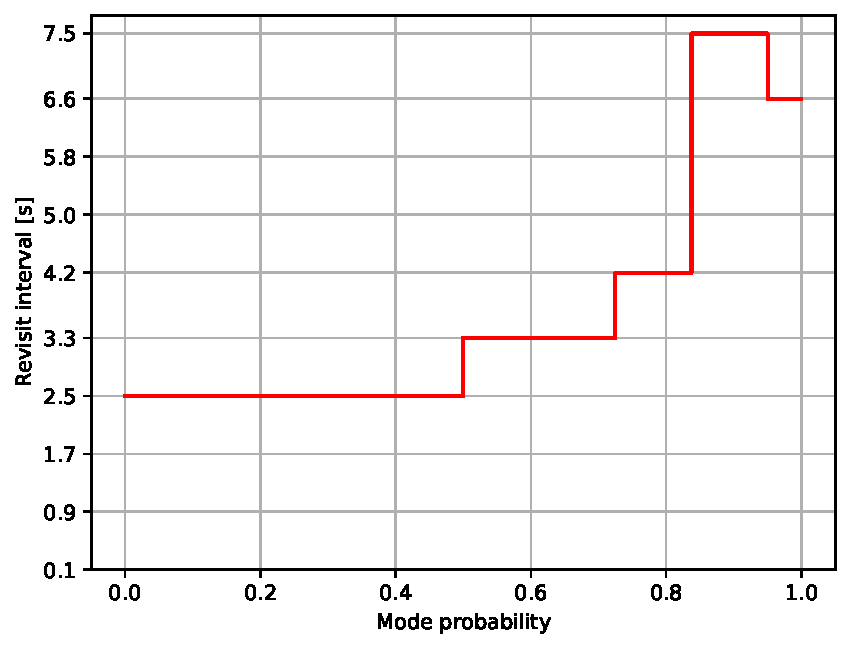
\includegraphics[width=.7\linewidth]{figures/benchmark/Simulations/policy.pdf}
    \caption{Policy for the agent with id=4. The state on x-axis is the mode probability, and the agent chooses the revisit interval on y-axis when in a corresponding state.}
    \label{fig:policy_id4}
\end{figure}

From figures \ref{fig:online_load} and \ref{fig:offline_load}, it can be seen that the agents using innovation based state presentation (ids from 0 to 3) perform worse than the agents with mode probability based state presentation (ids from 4 to 7).
Obviously, it needs to be accounted that only the agents with similar type of configuration, e.g. myopic policy with one dimensional state presentation, are comparable.
In terms of fast learning speed, low mean PLT and tracking load, the agent with $id=4$ is identified to have desirable performance.
The agent is using mode probabilities as a state space, and it is based on myopic policy.
The policy of the agent with $id=4$ is shown in Figure \ref{fig:policy_id4}.

Lastly, the agent with $id=4$ is trained and evaluated with various different $\closs$.
Figure \ref{fig:penalty_comparison} shows PLT for each trajectory and the mean tracking load with using various $\closs$.
As expected, using lower $\closs$ results in higher PLT and lower tracking load.
Figure \ref{fig:penalty_comparison} is used to find $\closs$ with equivalent PLT compared to the baseline algorithm. 

\begin{figure}[tb]
    \centering
    \begin{subfigure}[b]{0.45\textwidth}
        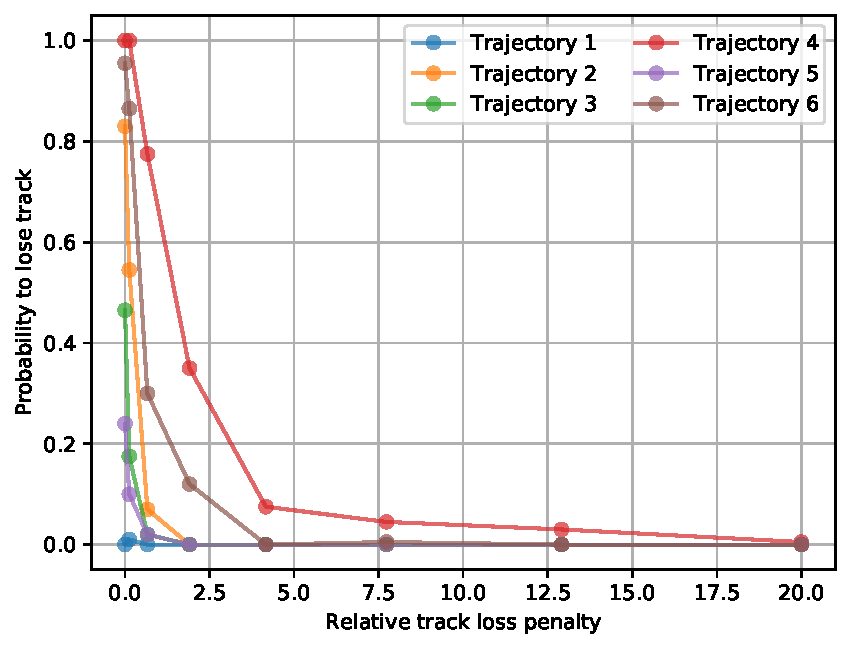
\includegraphics[width=\linewidth]{figures/benchmark/Simulations/plt_agent.pdf}
        \caption{Probability of losing a track.}
        \label{fig:penalty_plt}
    \end{subfigure}
    \hfill
    \begin{subfigure}[b]{0.45\textwidth}
        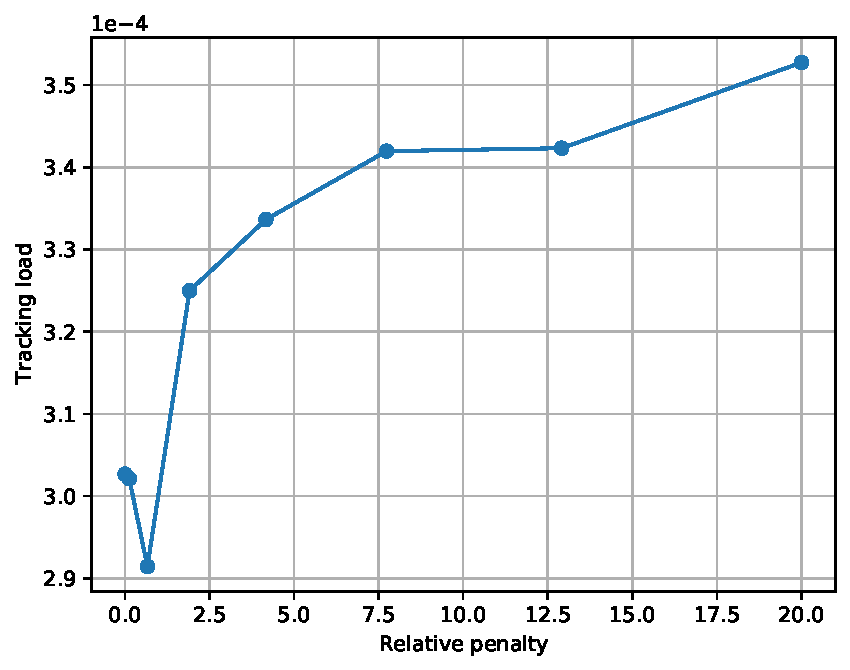
\includegraphics[width=\linewidth]{figures/benchmark/Training/tracking_load_agent.pdf}
        \caption{Mean tracking load.}
        \label{fig:penalty_load}
    \end{subfigure}
    \caption{Mean probability of losing a track for each trajectory and mean tracking load evaluated  with various tracking loss penalties. Relative track loss penalty is relative to tracking load with shortest revisit interval and single dwell.}
    \label{fig:penalty_comparison}
\end{figure}


\subsubsection{Performance against the baseline algorithm} \label{sec:against_baseline}

A RL agent and the baseline algorithm are compared in the benchmark problem by evaluating the tracking load as defined in equation \eqref{eq:load}.
In addition, error in predictive target position estimates $|\vec{p}-\hat{\vec{p}}|_2$ are visualized, where $\vec{p}$ is the target position and $\hat{\vec{p}}$ is the predicted target position.
Lastly, RI selections are shown to illustrate differences in RL agent and the baseline algorithm.

The agent with $id=4$ in Table \ref{tab:agent_configurations} is selected to the comparison since it was empirically identified to have desirable performance in Section \ref{sec:training}.
From figures \ref{fig:baseline_plt} and \ref{fig:penalty_plt}, the parameters $c_loss$ and $V_0$ can be selected to obtain fair comparison between the RL and the baseline algorithms.
Thus, the parameters $\closs = 0.2$ and $V_0=0.164$ were selected.
With the corresponding parameters RL agent lost target in trajectory 4 with the probability of $0.5\%$, and the baseline algorithm did not lose tracks in the Monte Carlo simulations with $1200$ iterations.

The tracking load is shown for each trajectory in Figure \ref{fig:tracking_load_comparison}.
For trajectories 1, 5 and 6 the tracking load of the baseline algorithm settles to similar tracking load values compared to the RL agent when the target is not maneuvering.
On the other hand, the RL agent can keep the load smaller on the turns where the tracking load peaks are induced.
In trajectories 2 and 3, the target approaches the radar such that the baseline algorithm decreases the RI gradually, leading into higher tracking loads than RL algorithm.
Based on the experience, the RL agent is confident enough that the corresponding situation does not require smaller RI such that lower tracking load is achieved.
In trajectory 4, difference between the baseline algorithm and RL algorithm is the most apparent.
As in with trajectories 2 and 3, the lower tracking load can be related to the distance of the trajectory.
The RL agent is more eager to take the risk of using longer RIs because the past experience does indicate that using such RIs does not have high risk of losing track.
However, the probability of losing track $0.5\%$ is higher than in other tracks because the state presentation may not generalize the corresponding track well enough.
It could be possible that the track is lost with lower probability if the target range would be included to the state.

In Figure \ref{fig:revisit_interval_comparison}, the selected RIs are shown for each benchmark trajectory.
The RIs of the RL algorithm are shorter than the baseline algorithm approximately at first 50 seconds of trajectories 1, 2 and 3.
However, significant tracking load difference is not shown in Figure \ref{fig:tracking_load_comparison}.
Thus, the reward function explicitly minimizing the immediate tracking load seems to work as intended because longer RIs can increase the number of dwells needed to achieve a detection.
Another major difference in all of the trajectories is that the baseline algorithm quite often uses shorter RIs when the target is maneuvering.
Those shorter RIs affect significantly to the tracking load as shown in Figure \ref{fig:tracking_load_comparison}.

Figure \ref{fig:position_error_comparison} shows the error in predictive target position estimates.
The error for the baseline and the RL algorithms are mostly similar except for the trajectory 4.
In trajectory 4, the error is higher since RL agent is using longer revisit intervals.
It explains why RL agent loses the trajectory 4 a little bit more often than the baseline algorithm does.


\begin{figure}[htb]
    \centering
    \begin{subfigure}[b]{0.45\textwidth}
        \centering
        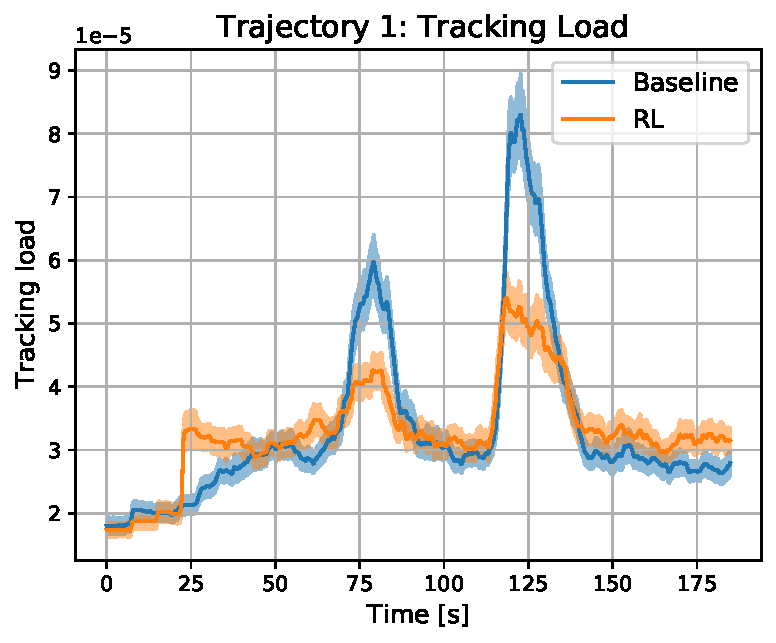
\includegraphics[width=\linewidth]{figures/benchmark/Simulations/tracking_load_0.pdf}
        \caption{Trajectory 1.}
        \label{fig:TL_T1}
    \end{subfigure}
    \hfill
    \begin{subfigure}[b]{0.45\textwidth}
        \centering
        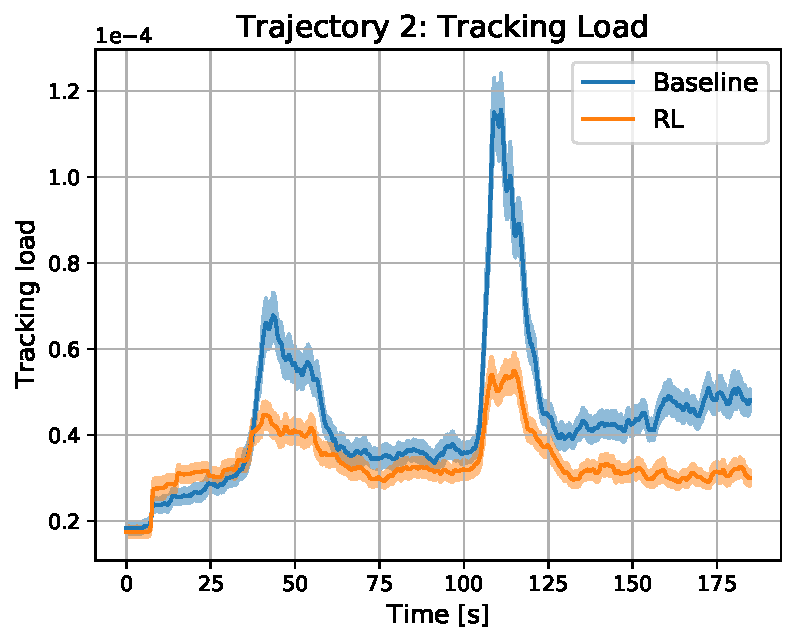
\includegraphics[width=\linewidth]{figures/benchmark/Simulations/tracking_load_1.pdf}
        \caption{Trajectory 2.}
        \label{fig:TL_T2}
    \end{subfigure}
    \hfill
    \begin{subfigure}[b]{0.45\textwidth}
        \centering
        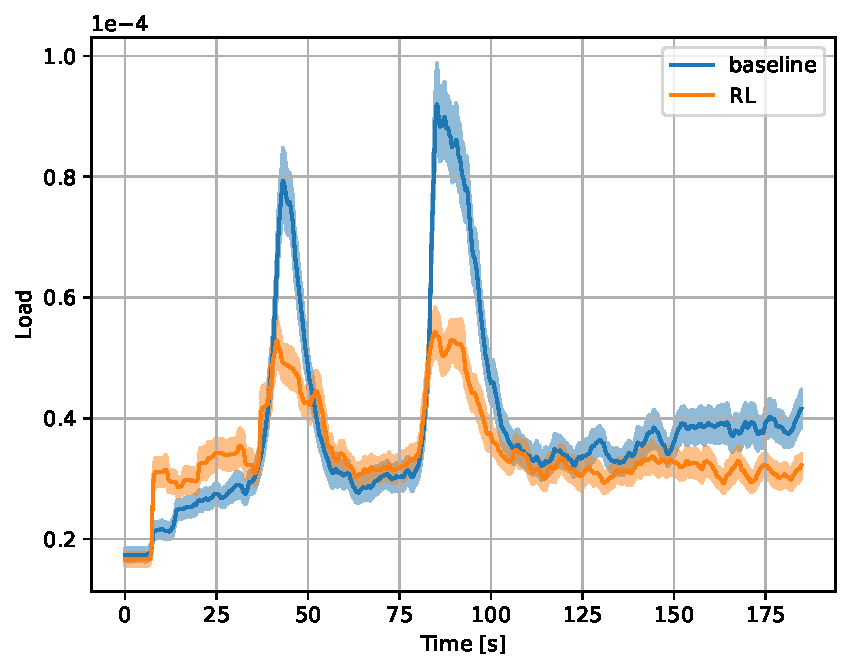
\includegraphics[width=\linewidth]{figures/benchmark/Simulations/tracking_load_2.pdf}
        \caption{Trajectory 3.}
        \label{fig:TL_T3}
    \end{subfigure}
    \hfill
    \begin{subfigure}[b]{0.45\textwidth}
        \centering
        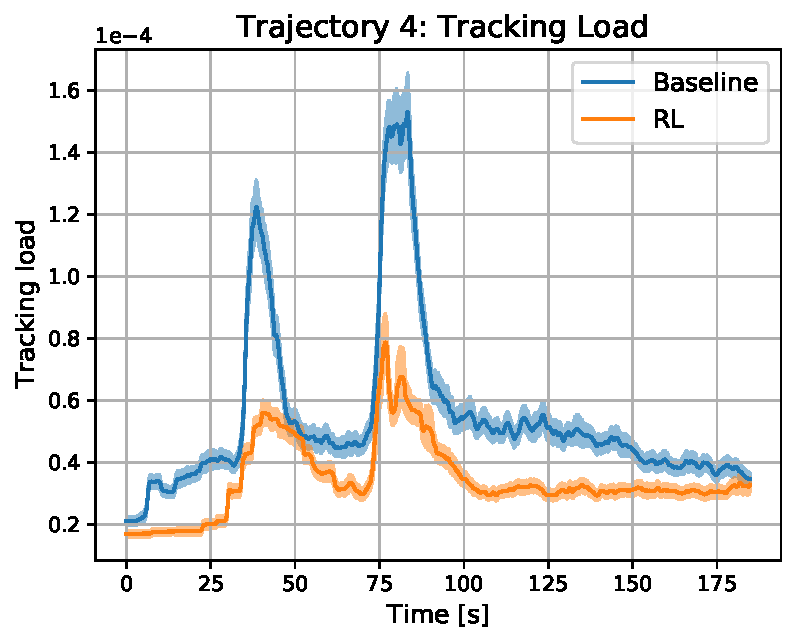
\includegraphics[width=\linewidth]{figures/benchmark/Simulations/tracking_load_3.pdf}
        \caption{Trajectory 4.}
        \label{fig:TL_T4}
    \end{subfigure}
    \hfill
    \begin{subfigure}[b]{0.45\textwidth}
        \centering
        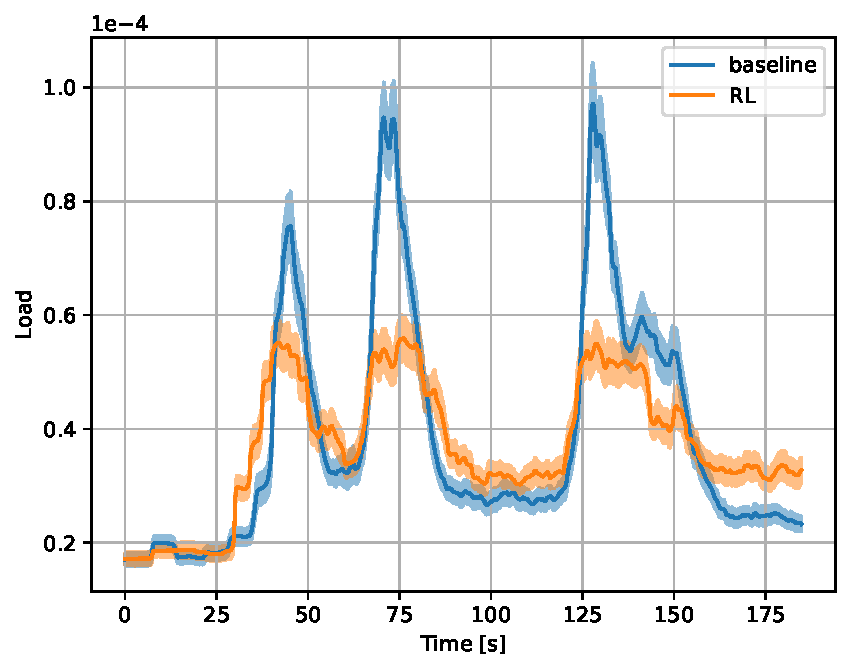
\includegraphics[width=\linewidth]{figures/benchmark/Simulations/tracking_load_4.pdf}
        \caption{Trajectory 5.}
        \label{fig:TL_T5}
    \end{subfigure}
    \hfill
    \begin{subfigure}[b]{0.45\textwidth}
        \centering
        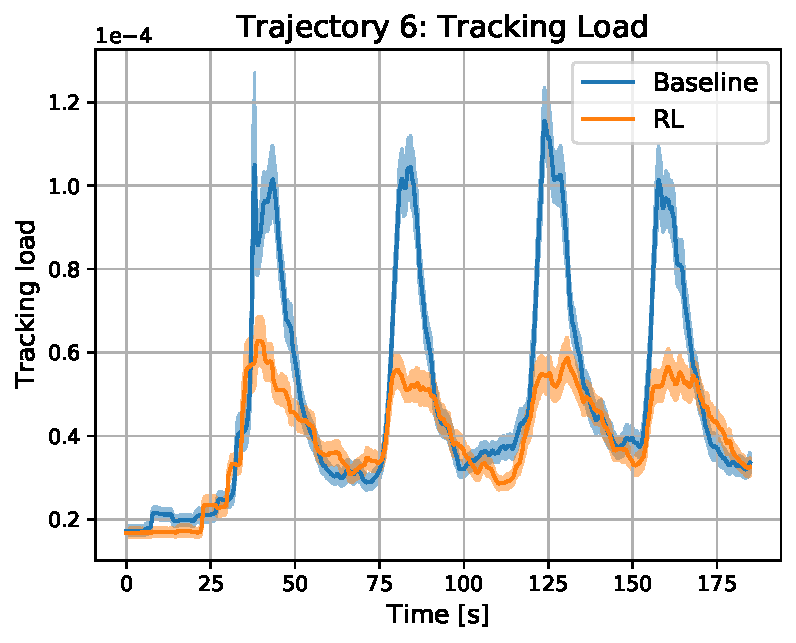
\includegraphics[width=\linewidth]{figures/benchmark/Simulations/tracking_load_5.pdf}
        \caption{Trajectory 6.}
        \label{fig:TL_T6}
    \end{subfigure}
    \caption{Comparing the proposed reinforcement learning approach to the baseline algorithm in terms of tracking load.
    The figures provide expected tracking load with 95\% confidence intervals.}
    \label{fig:tracking_load_comparison}
\end{figure}

\begin{figure}[htb]
    \centering
    \begin{subfigure}[b]{0.45\textwidth}
        \centering
        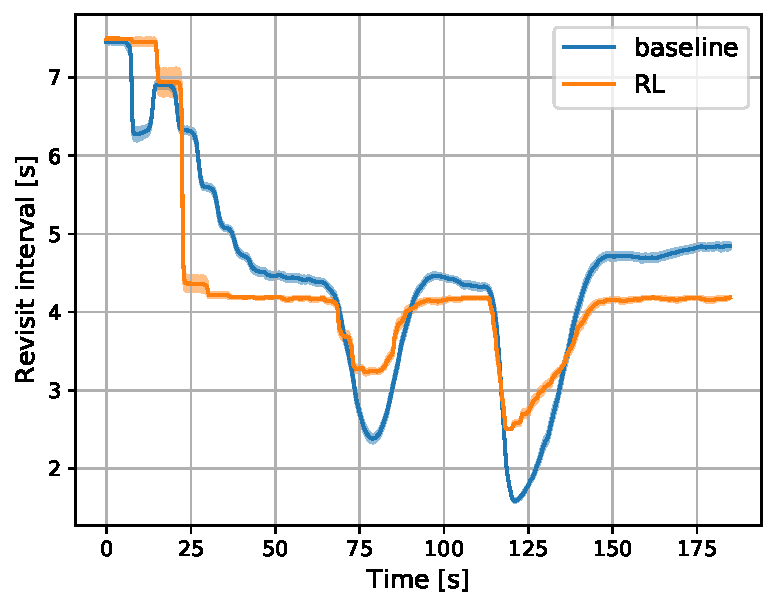
\includegraphics[width=\linewidth]{figures/benchmark/Simulations/revisit_intervals_0.pdf}
        \caption{Trajectory 1.}
        \label{fig:RI_T1}
    \end{subfigure}
    \hfill
    \begin{subfigure}[b]{0.45\textwidth}
        \centering
        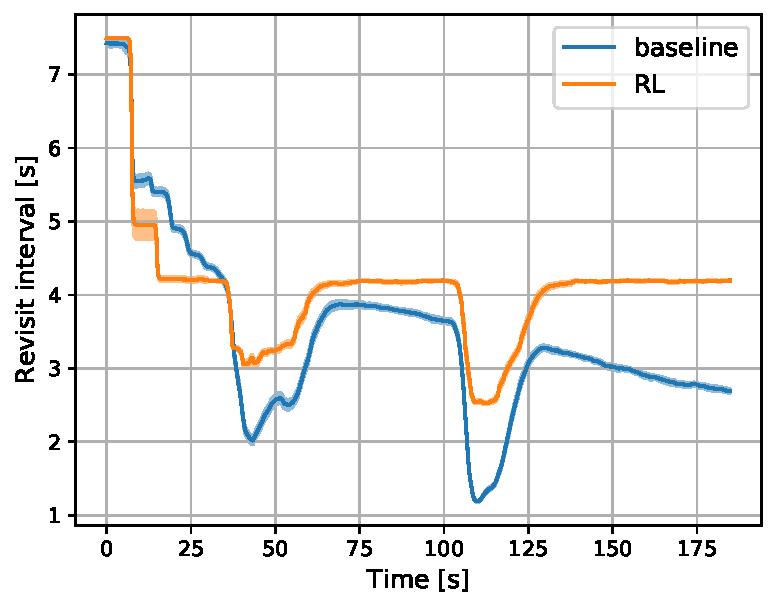
\includegraphics[width=\linewidth]{figures/benchmark/Simulations/revisit_intervals_1.pdf}
        \caption{Trajectory 2.}
        \label{fig:RI_T2}
    \end{subfigure}
    \hfill
    \begin{subfigure}[b]{0.45\textwidth}
        \centering
        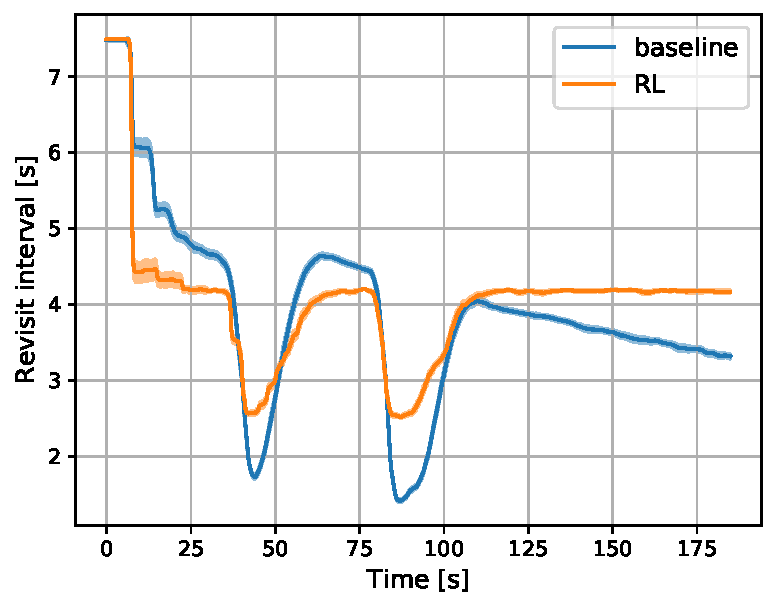
\includegraphics[width=\linewidth]{figures/benchmark/Simulations/revisit_intervals_2.pdf}
        \caption{Trajectory 3.}
        \label{fig:RI_T3}
    \end{subfigure}
    \hfill
    \begin{subfigure}[b]{0.45\textwidth}
        \centering
        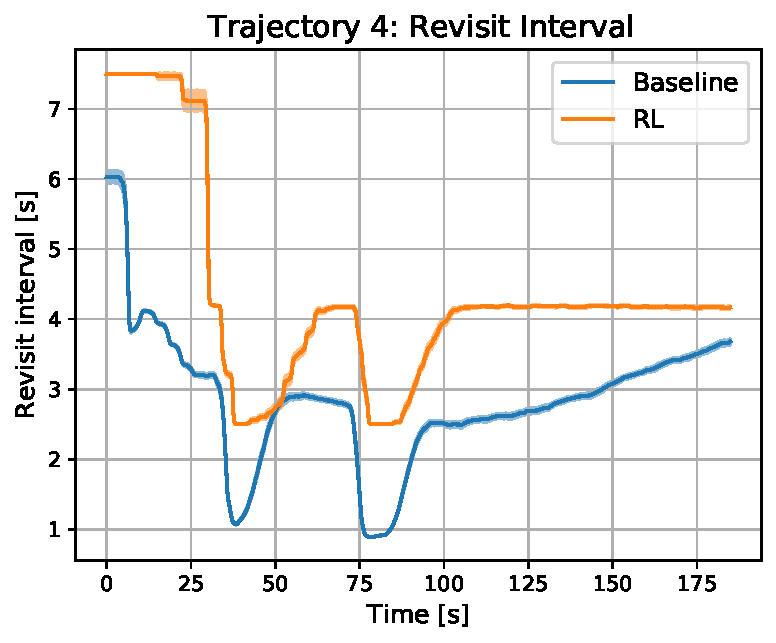
\includegraphics[width=\linewidth]{figures/benchmark/Simulations/revisit_intervals_3.pdf}
        \caption{Trajectory 4.}
        \label{fig:RI_T4}
    \end{subfigure}
    \hfill
    \begin{subfigure}[b]{0.45\textwidth}
        \centering
        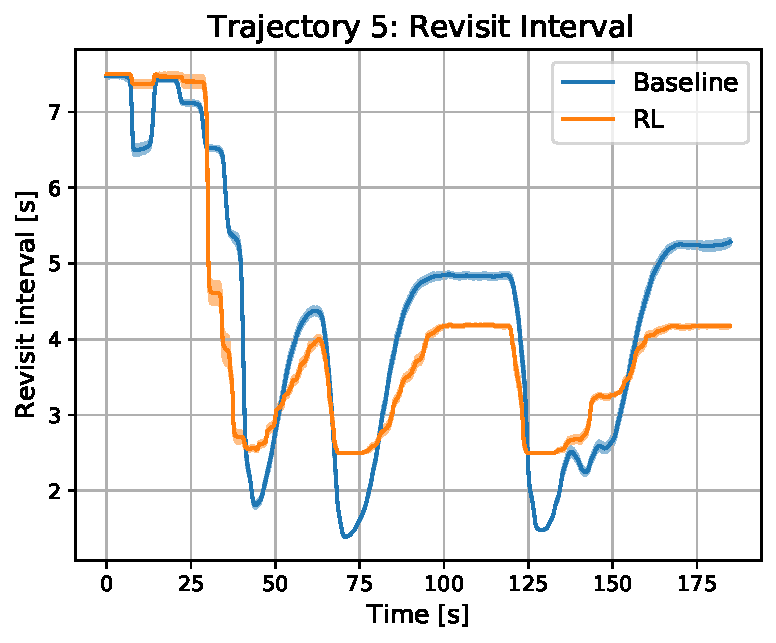
\includegraphics[width=\linewidth]{figures/benchmark/Simulations/revisit_intervals_4.pdf}
        \caption{Trajectory 5.}
        \label{fig:RI_T5}
    \end{subfigure}
    \hfill
    \begin{subfigure}[b]{0.45\textwidth}
        \centering
        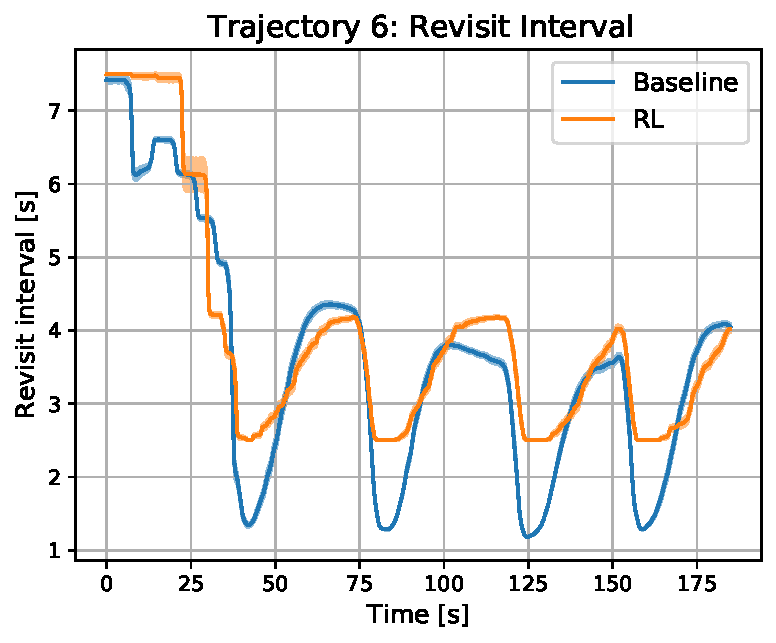
\includegraphics[width=\linewidth]{figures/benchmark/Simulations/revisit_intervals_5.pdf}
        \caption{Trajectory 6.}
        \label{fig:RI_T6}
    \end{subfigure}
    \caption{Comparing the proposed reinforcement learning approach to the baseline algorithm in terms of revisit intervals.
    The figures provide expected revisit interval with 95\% confidence intervals.}
    \label{fig:revisit_interval_comparison}
\end{figure}

\begin{figure}[htb]
    \centering
    \begin{subfigure}[b]{0.45\textwidth}
        \centering
        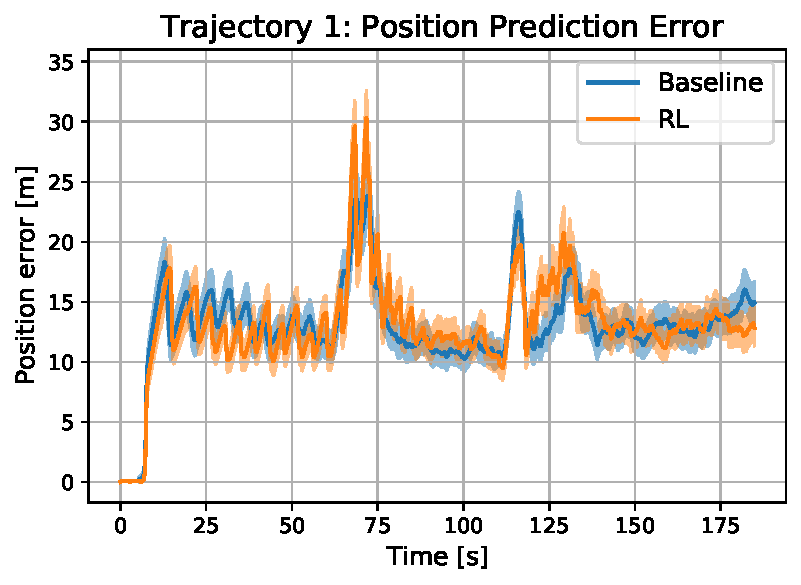
\includegraphics[width=\linewidth]{figures/benchmark/Simulations/mean_position_error0.pdf}
        \caption{Trajectory 1.}
        \label{fig:PE_T1}
    \end{subfigure}
    \hfill
    \begin{subfigure}[b]{0.45\textwidth}
        \centering
        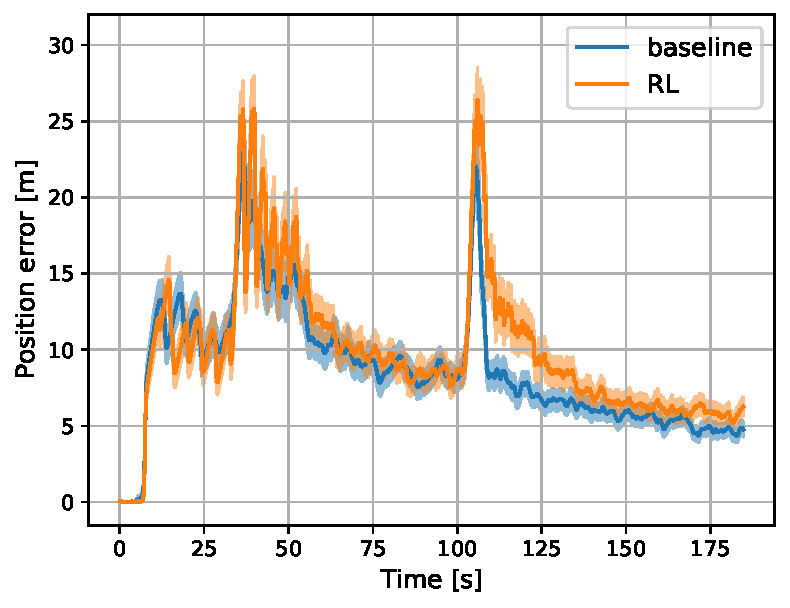
\includegraphics[width=\linewidth]{figures/benchmark/Simulations/mean_position_error1.pdf}
        \caption{Trajectory 2.}
        \label{fig:PE_T2}
    \end{subfigure}
    \hfill
    \begin{subfigure}[b]{0.45\textwidth}
        \centering
        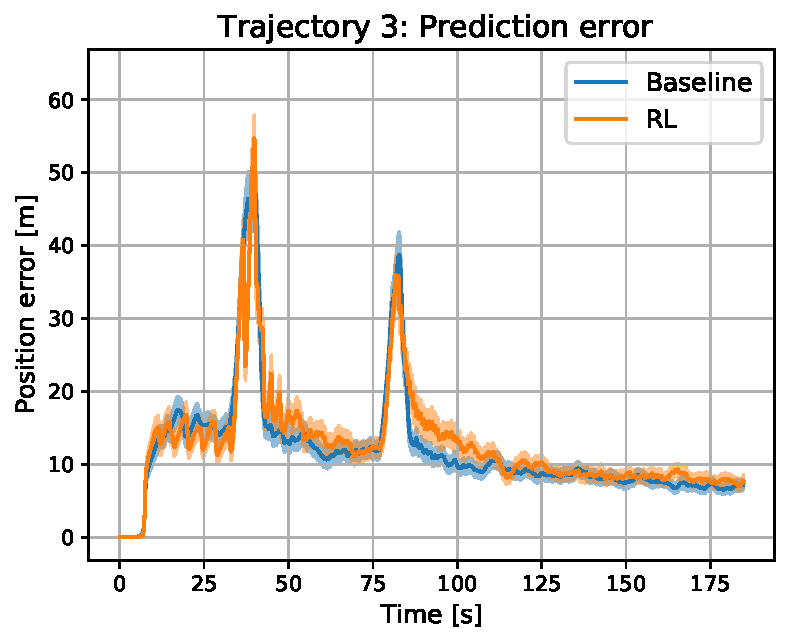
\includegraphics[width=\linewidth]{figures/benchmark/Simulations/mean_position_error2.pdf}
        \caption{Trajectory 3.}
        \label{fig:PE_T3}
    \end{subfigure}
    \hfill
    \begin{subfigure}[b]{0.45\textwidth}
        \centering
        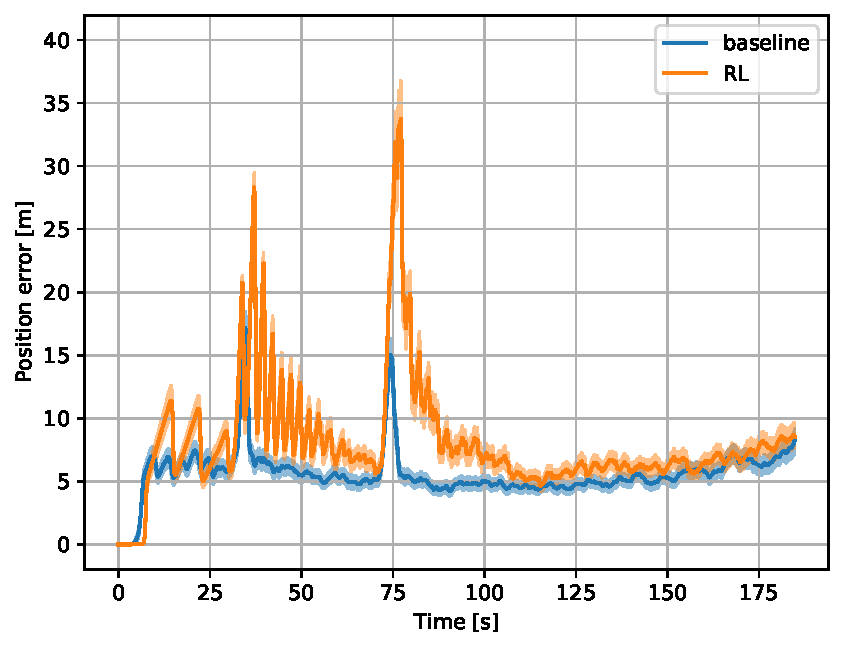
\includegraphics[width=\linewidth]{figures/benchmark/Simulations/mean_position_error3.pdf}
        \caption{Trajectory 4.}
        \label{fig:PE_T4}
    \end{subfigure}
    \hfill
    \begin{subfigure}[b]{0.45\textwidth}
        \centering
        \includegraphics[width=\linewidth]{figures/benchmark/Simulations/mean_position_error4.pdf}
        \caption{Trajectory 5.}
        \label{fig:PE_T5}
    \end{subfigure}
    \hfill
    \begin{subfigure}[b]{0.45\textwidth}
        \centering
        \includegraphics[width=\linewidth]{figures/benchmark/Simulations/mean_position_error5.pdf}
        \caption{Trajectory 6.}
        \label{fig:PE_T6}
    \end{subfigure}
    \caption{Comparing the proposed reinforcement learning approach to the baseline algorithm in terms of error in predictive target position estimates.
    The figures provide expected revisit interval with 95\% confidence intervals.}
    \label{fig:position_error_comparison}
\end{figure}


\subsection{Summary}

The RIS was formulated as a RL problem by identifying suitable states, actions and rewards for the problem at hand.
Q-learning algorithm with \egreedy exploration was utilized to solve RIS problem.
The different RL configurations were evaluated using the benchmark trajectories in terms of offline and online performance in addition to comparing the most promising RL configurations to the baseline algorithm.
It was found that the performance of the RL agent is comparable to the baseline algorithm.
In addition, the proposed learning-based approach can benefit from utilizing the past experience to reduce tracking load peaks compared to the baseline algorithm.
Future research directions could include function approximation techniques that could enable applying higher dimension state spaces more efficiently. 
In addition, more efficient exploration strategies from the MAB framework could be investigated especially when using the myopic policies.


\newpage
\section{Conclusions} \label{sec:conclusions}

In this thesis RRM subproblems were formulated as RL problems which were solved using RL methods. 
Since RRM contain multiple subproblems, only two distinct subproblems were considered. 
The RL approaches were evaluated in Monte Carlo simulations and compared to baseline algorithms. 
In both applications, the RL approaches did improve the performance through the experience, and with sufficient amount of learning an advantage can be seen compared to the baseline algorithms.

In TX-RX selection for distributed MIMO radars, MAB framework was utilized to learn select subset of TXs and RXs that have highest total SINR in linear scale. 
Furthermore, the problem was modeled as combinatorial MAB problem, that was used to reduce the dimensions of the action space.  
Each arm in the MAB formulation was modeled as  single TX-RX pair such that the RL agent selects multiple arms at a time. 
The exploration-exploitation trade-off ensured that all the different TX-RX pairs were probed for sufficient number of times in order to minimize the regret. 
For moving target scenarios, constant discount factor was used to weight past observations less than recent observations. 
It was found out that using the RL approach, the total SINR was close to optimal even in non-stationary scenarios and outperformed the exploration-free approach. 
However, the limitation of RL approach is that radar is assumed to be able to probe different subsets with a high sampling rate.
Contextual multi-armed bandits could be used to address the non-stationary reward distributions and enable using RL even with lower sampling rates. 

The RIS was addressed with general RL framework such that the observations, the actions and the rewards were defined. Various RL agents were configured differently to identify efficient state space presentation in terms of learning speed and performance. 
In addition, non-myopic and myopic agents were evaluated to find out if myopic policy is sufficient for the problem at hand. 
The Q-learning algorithm with epsilon-greedy exploration was used to solve the RL problem in which rewards were based on tracking loads and penalties when losing tracks. 
It was identified that myopic policy is sufficient such that the learning speed can be improved. 
The RL approach was able to reduce the tracking load peaks which is important when working on overload situations.
However, the learning speed was significantly decreased when increasing number of states.
Learning speed could be improved by applying function approximators to estimate generalize states-action pairs which the agent have not seen before.  
In addition, it would be possible to utilize more efficient policies to handle the exploration- exploitation trade-off especially in myopic case.
In future research, RIS could be extended by applying RL for controlling the dwell times which were currently assumed constant.

Both of the RRM subproblems were evaluated in STT scenario such that formulating the RRM subproblems as RL formulations were less complicated. 
In future research, also the MTT scenario should be considered. 
It would require taking in account scheduling in both problems as well as track association in the RIS problem. 






\thesisbibliography

\printbibliography


\end{document}
